%%%%%%%%%%%%%%%%%%%%%%%%%%%%%%%%%
% Iterations                    %
%%%%%%%%%%%%%%%%%%%%%%%%%%%%%%%%%

\section{Iterations}

This chapter presents in detail the four iterations through which the artifacts of the project were produced. As established in the previous chapter, each iteration follows the Design Science Research regulative cycle and is developed through its five activities, from problem investigation to solution evaluation. The chapter proceeds iteration by iteration, from the maturity framework of Iteration~1 to the multi-tenant platform of Iteration~4, and closes with the detailed use case specifications of the delivered platform.

\subsection{Iteration 1: Designing the Maturity Framework}

The first iteration designs the data maturity assessment framework, the reference structure against which every later iteration is measured. Following the regulative cycle, it proceeds through the five activities below, from problem investigation to solution evaluation.

\subsubsection{Problem Investigation}

The diagnostic established that the sector lacks a structured way to describe what data maturity means in a banking context. The first iteration therefore addresses the problem of defining a comprehensive yet applicable structure of dimensions, sub-dimensions, and indicators that covers the breadth of data management while remaining aligned with the regulatory expectations.

\subsubsection{Solution Design}

The framework was designed as a three level hierarchy: five dimensions, decomposed into twelve sub-dimensions, themselves assessed through 47 indicators. The five dimensions are Governance, Data Quality, Architecture and Access, Analytics and Tools, and Skills and Culture. Each component was drawn from the most appropriate benchmark source, with DAMA-DMBOK providing the structural backbone and DCAM providing the regulatory anchor that ties the framework to the BCT and BCBS 239 requirements.

The five dimensions were not chosen arbitrarily; each answers a distinct question that a banking supervisor or a chief data officer must be able to answer with evidence. Governance (D1) asks whether the institution has a mandate, an accountable owner, and a compliance posture for its data, and it carries the heaviest weight because it is the precondition for every other capability and the focus of the BCT Circulaire N\textdegree{}2025-08. It is decomposed into three sub-dimensions, Strategy and data policy (1.1), Ownership and responsibilities (1.2), and Regulatory compliance (1.3), and holds twelve indicators, the most of any dimension. Data Quality (D2) asks whether the data on which decisions and regulatory reports rest is complete, accurate, timely, controlled, and traceable; its three sub-dimensions are Quality dimensions (2.1), Controls and processes (2.2), and Lineage and traceability (2.3), assessed through eleven indicators. Architecture and Access (D3) asks whether data is centralized, integrated, and served through governed pipelines with controlled access; it groups Centralization and integration (3.1) and Pipelines and infrastructure (3.2) into eight indicators. Analytics and Tools (D4) asks whether the institution can turn its data into decisions through modern platforms and actual usage; it groups Tool maturity (4.1) and Data usage (4.2) into eight indicators. Skills and Culture (D5) asks whether the organization has the human capability and the cultural adoption to sustain the other four dimensions; it groups Data skills (5.1) and Culture and adoption (5.2) into eight indicators and is treated as a proxy dimension, meaning it is measured indirectly through observable stand-ins such as training budget, headcount ratio, and certifications rather than by direct self-assessment, as explained in the evaluation below. The full list of the twelve sub-dimensions and the 47 indicators, each with its five-level scoring rubric, is catalogued in Appendix~A.

Within each sub-dimension the indicators were designed according to three principles. First, every indicator must be answerable from an artifact that a bank already possesses or can produce, such as an approved policy, a system log, a dashboard, or a measured ratio, so that the assessment never reduces to opinion. Second, each indicator carries a five level rubric that describes, in plain language, exactly what a bank must demonstrate to earn each score from one to five, which turns a subjective scale into a set of observable, auditable conditions. Third, indicators that correspond to a specific regulatory obligation are flagged so that the tool can enforce their special treatment, which yields the thirteen non-skippable regulatory indicators discussed below.

The distribution of the five dimension weights across the Global Maturity Index is shown in Figure~\ref{fig:weight-distribution}. The heaviest allocation to Governance reflects both its foundational role and its regulatory centrality, while Data Quality, Architecture and Access, and Analytics and Tools each receive an equal share, and Skills and Culture receives the smallest share consistent with its proxy nature.

\begin{figure}[H]
\centering
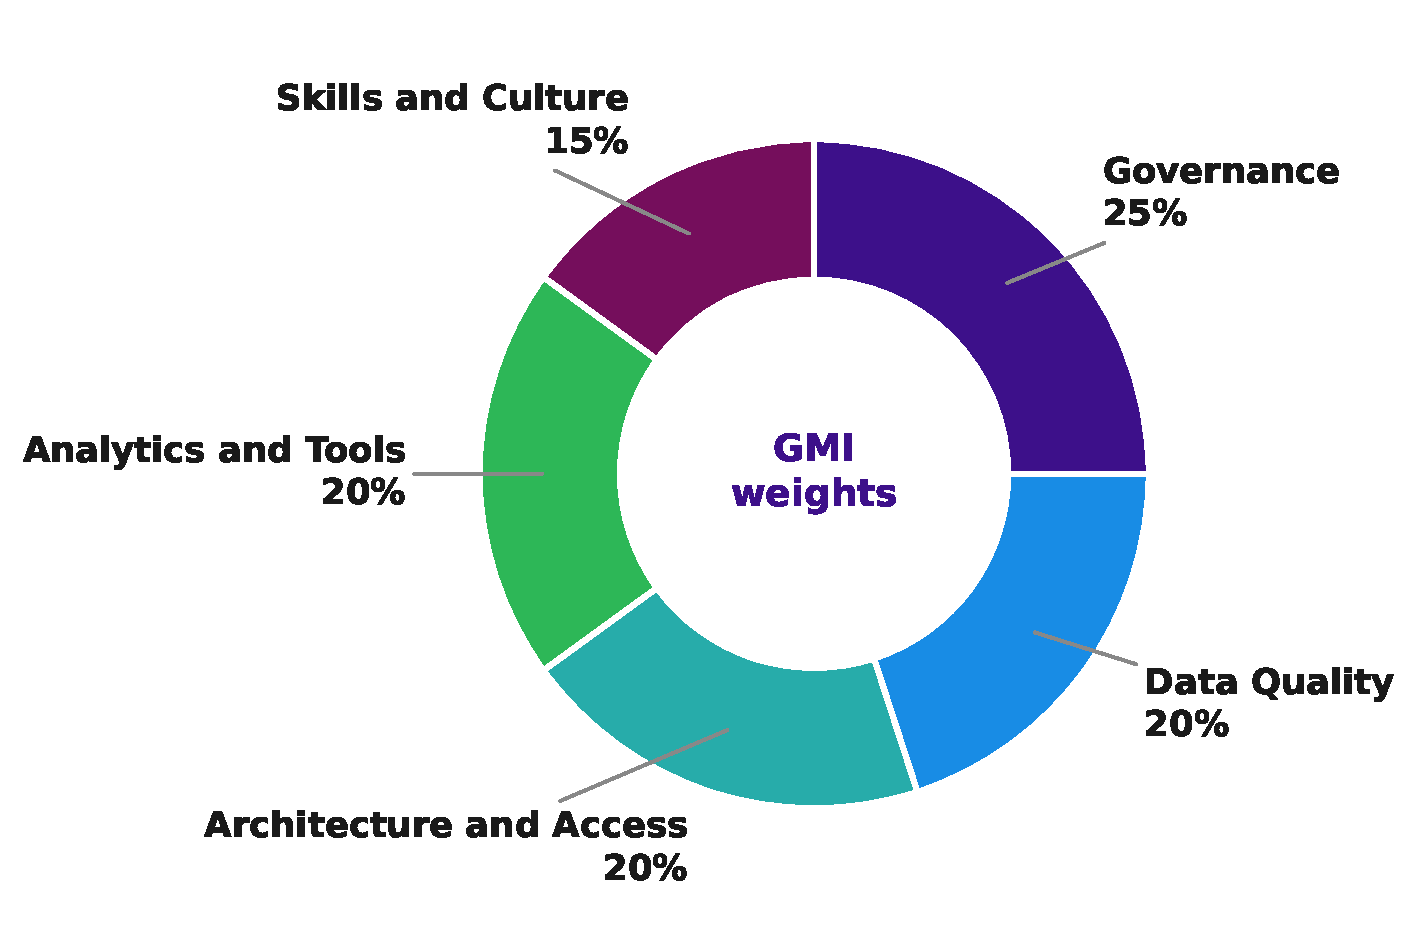
\includegraphics[width=0.7\textwidth]{images/weight-distribution.pdf}
\caption{Distribution of the five dimension weights in the Global Maturity Index}
\label{fig:weight-distribution}
\end{figure}

\subsubsection{Design Validation}

The design was validated against two requirements: completeness, in that the dimensions cover the full scope of data management identified in the literature, and regulatory alignment, in that every governance and quality expectation of the BCT and BCBS 239 maps onto at least one indicator. The distribution of indicators and the weighting of dimensions were reviewed to ensure that governance, which carries the highest regulatory importance, carries the highest weight.

Beyond these two requirements, two design risks were assessed before the indicator catalogue was written, and the worst case of each was traced on paper. The first risk is a coverage hole: a data management concern present in the retained source frameworks but absent from the hierarchy would silently escape every future assessment. This was checked by mapping each domain retained from the benchmark onto at least one sub-dimension of the tree, so that no retained concern lacks a place where it is scored. The second risk is regulatory dilution, whose worst case takes two forms: a regulatory obligation that lands only on a skippable indicator, which a respondent could then evade, or one that lands inside the proxy dimension, where it would be assessed only indirectly. Locating each of the thirteen regulatory indicators within the structure confirmed that neither case arises: all thirteen sit in the four directly assessed dimensions, Skills and Culture carries none, and the regulatory flag attached to each of them is precisely what allows the following iteration to make them non-skippable. The concrete instrument of this validation was the one-to-one mapping exercise itself, which forced every regulatory expectation to name the indicator that answers it.

The weighting scheme allocates 25\% to Governance, 20\% each to Data Quality, Architecture and Access, and Analytics and Tools, and 15\% to Skills and Culture. This scheme was validated on two grounds. First, Governance is the enabling dimension: without an approved strategy, accountable owners, and a compliance posture, the improvements measured by the other dimensions cannot be sustained, which justifies its dominant weight. Second, Skills and Culture receives the lowest weight because it is assessed through proxy indicators rather than direct self reported maturity, so a slightly smaller contribution to the global index limits the influence of the least directly observable dimension. The three intermediate dimensions receive an identical weight because no evidence in the diagnostic justified ranking data quality, architecture, or analytics above one another; treating them symmetrically keeps the index neutral and defensible.

Regulatory alignment was validated by locating each of the thirteen regulatory indicators within the dimension structure. Governance concentrates the largest share of regulatory obligations, followed by Data Quality, then Architecture and Access and Analytics and Tools, while Skills and Culture carries none, which is consistent with its proxy status. The exact distribution of the thirteen regulatory indicators across the five dimensions is shown in Figure~\ref{fig:bct-coverage}, confirming that the regulatory load is concentrated where the BCT Circulaire N\textdegree{}2025-08 and BCBS 239 place their strongest expectations. The complete mapping of each of the thirteen regulatory indicators to the specific BCT or BCBS 239 obligation it operationalizes is given in Appendix~B.

\begin{figure}[H]
\centering
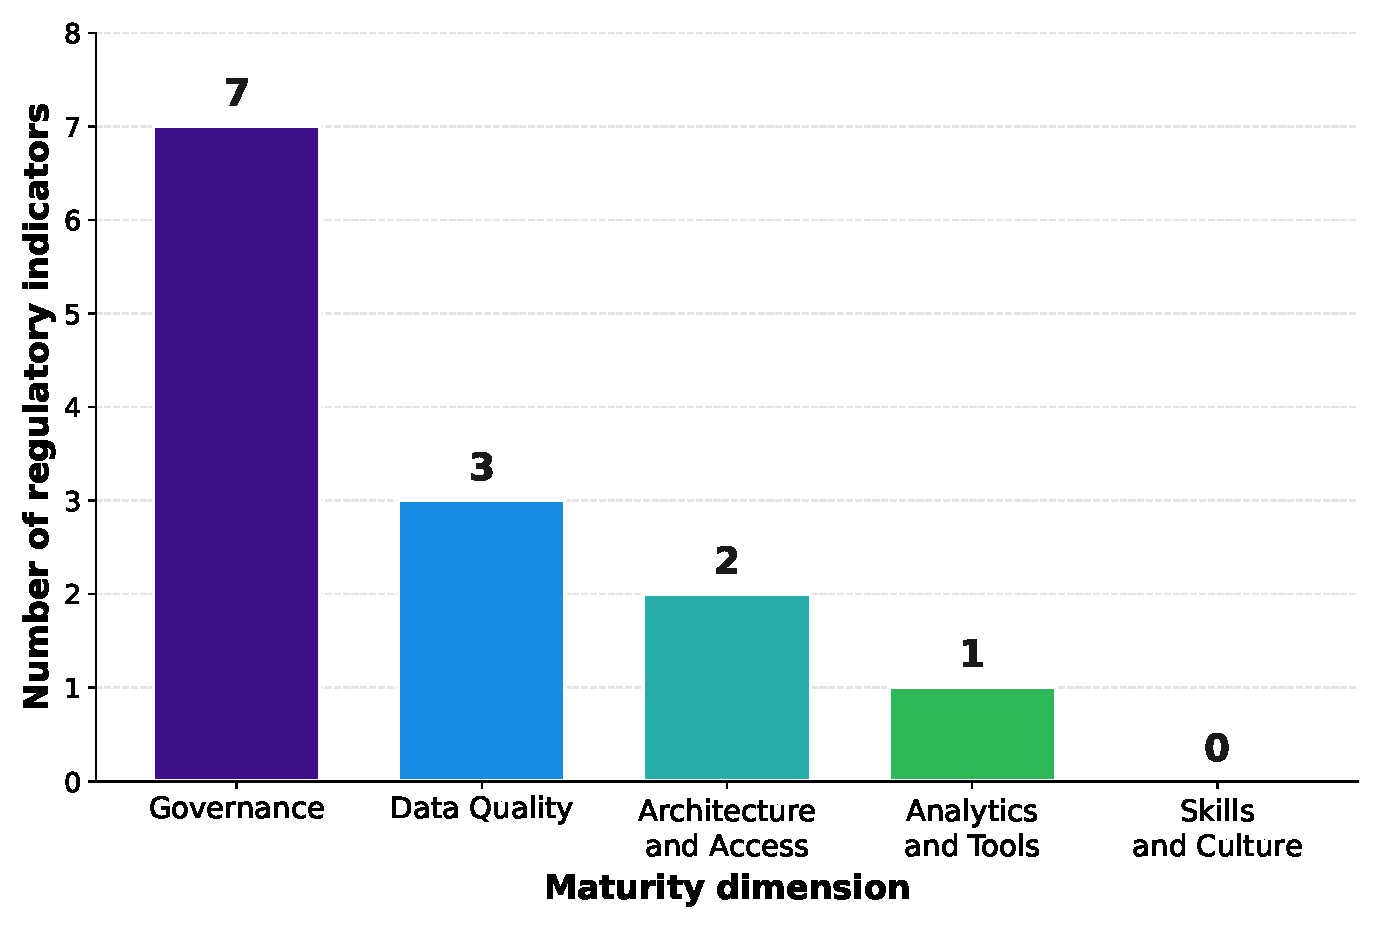
\includegraphics[width=0.75\textwidth]{images/bct-coverage.pdf}
\caption{Coverage of the thirteen regulatory indicators across the five dimensions}
\label{fig:bct-coverage}
\end{figure}

\subsubsection{Solution Implementation}

The framework was implemented as a structured catalogue of the 47 indicators\footnote{The full per-indicator scoring rubrics, giving the five levels of every one of the 47 indicators organized by dimension and sub-dimension, are listed in Appendix~A.}, each attached to its sub-dimension and dimension, and each accompanied by a plain-language question, a guidance hint, and a five level scoring rubric defining precisely what each score level means for that indicator. The full scoring rubrics for all indicators, organized by dimension and sub-dimension, are presented in Appendix A. The five dimensions, their weights, their number of sub-dimensions and indicators, and their primary sources are summarized in Table~\ref{tab:dimensions}.

The hierarchical structure of the complete framework is visualized in Figure~\ref{fig:framework-tree}.

\begin{figure}[H]
\centering
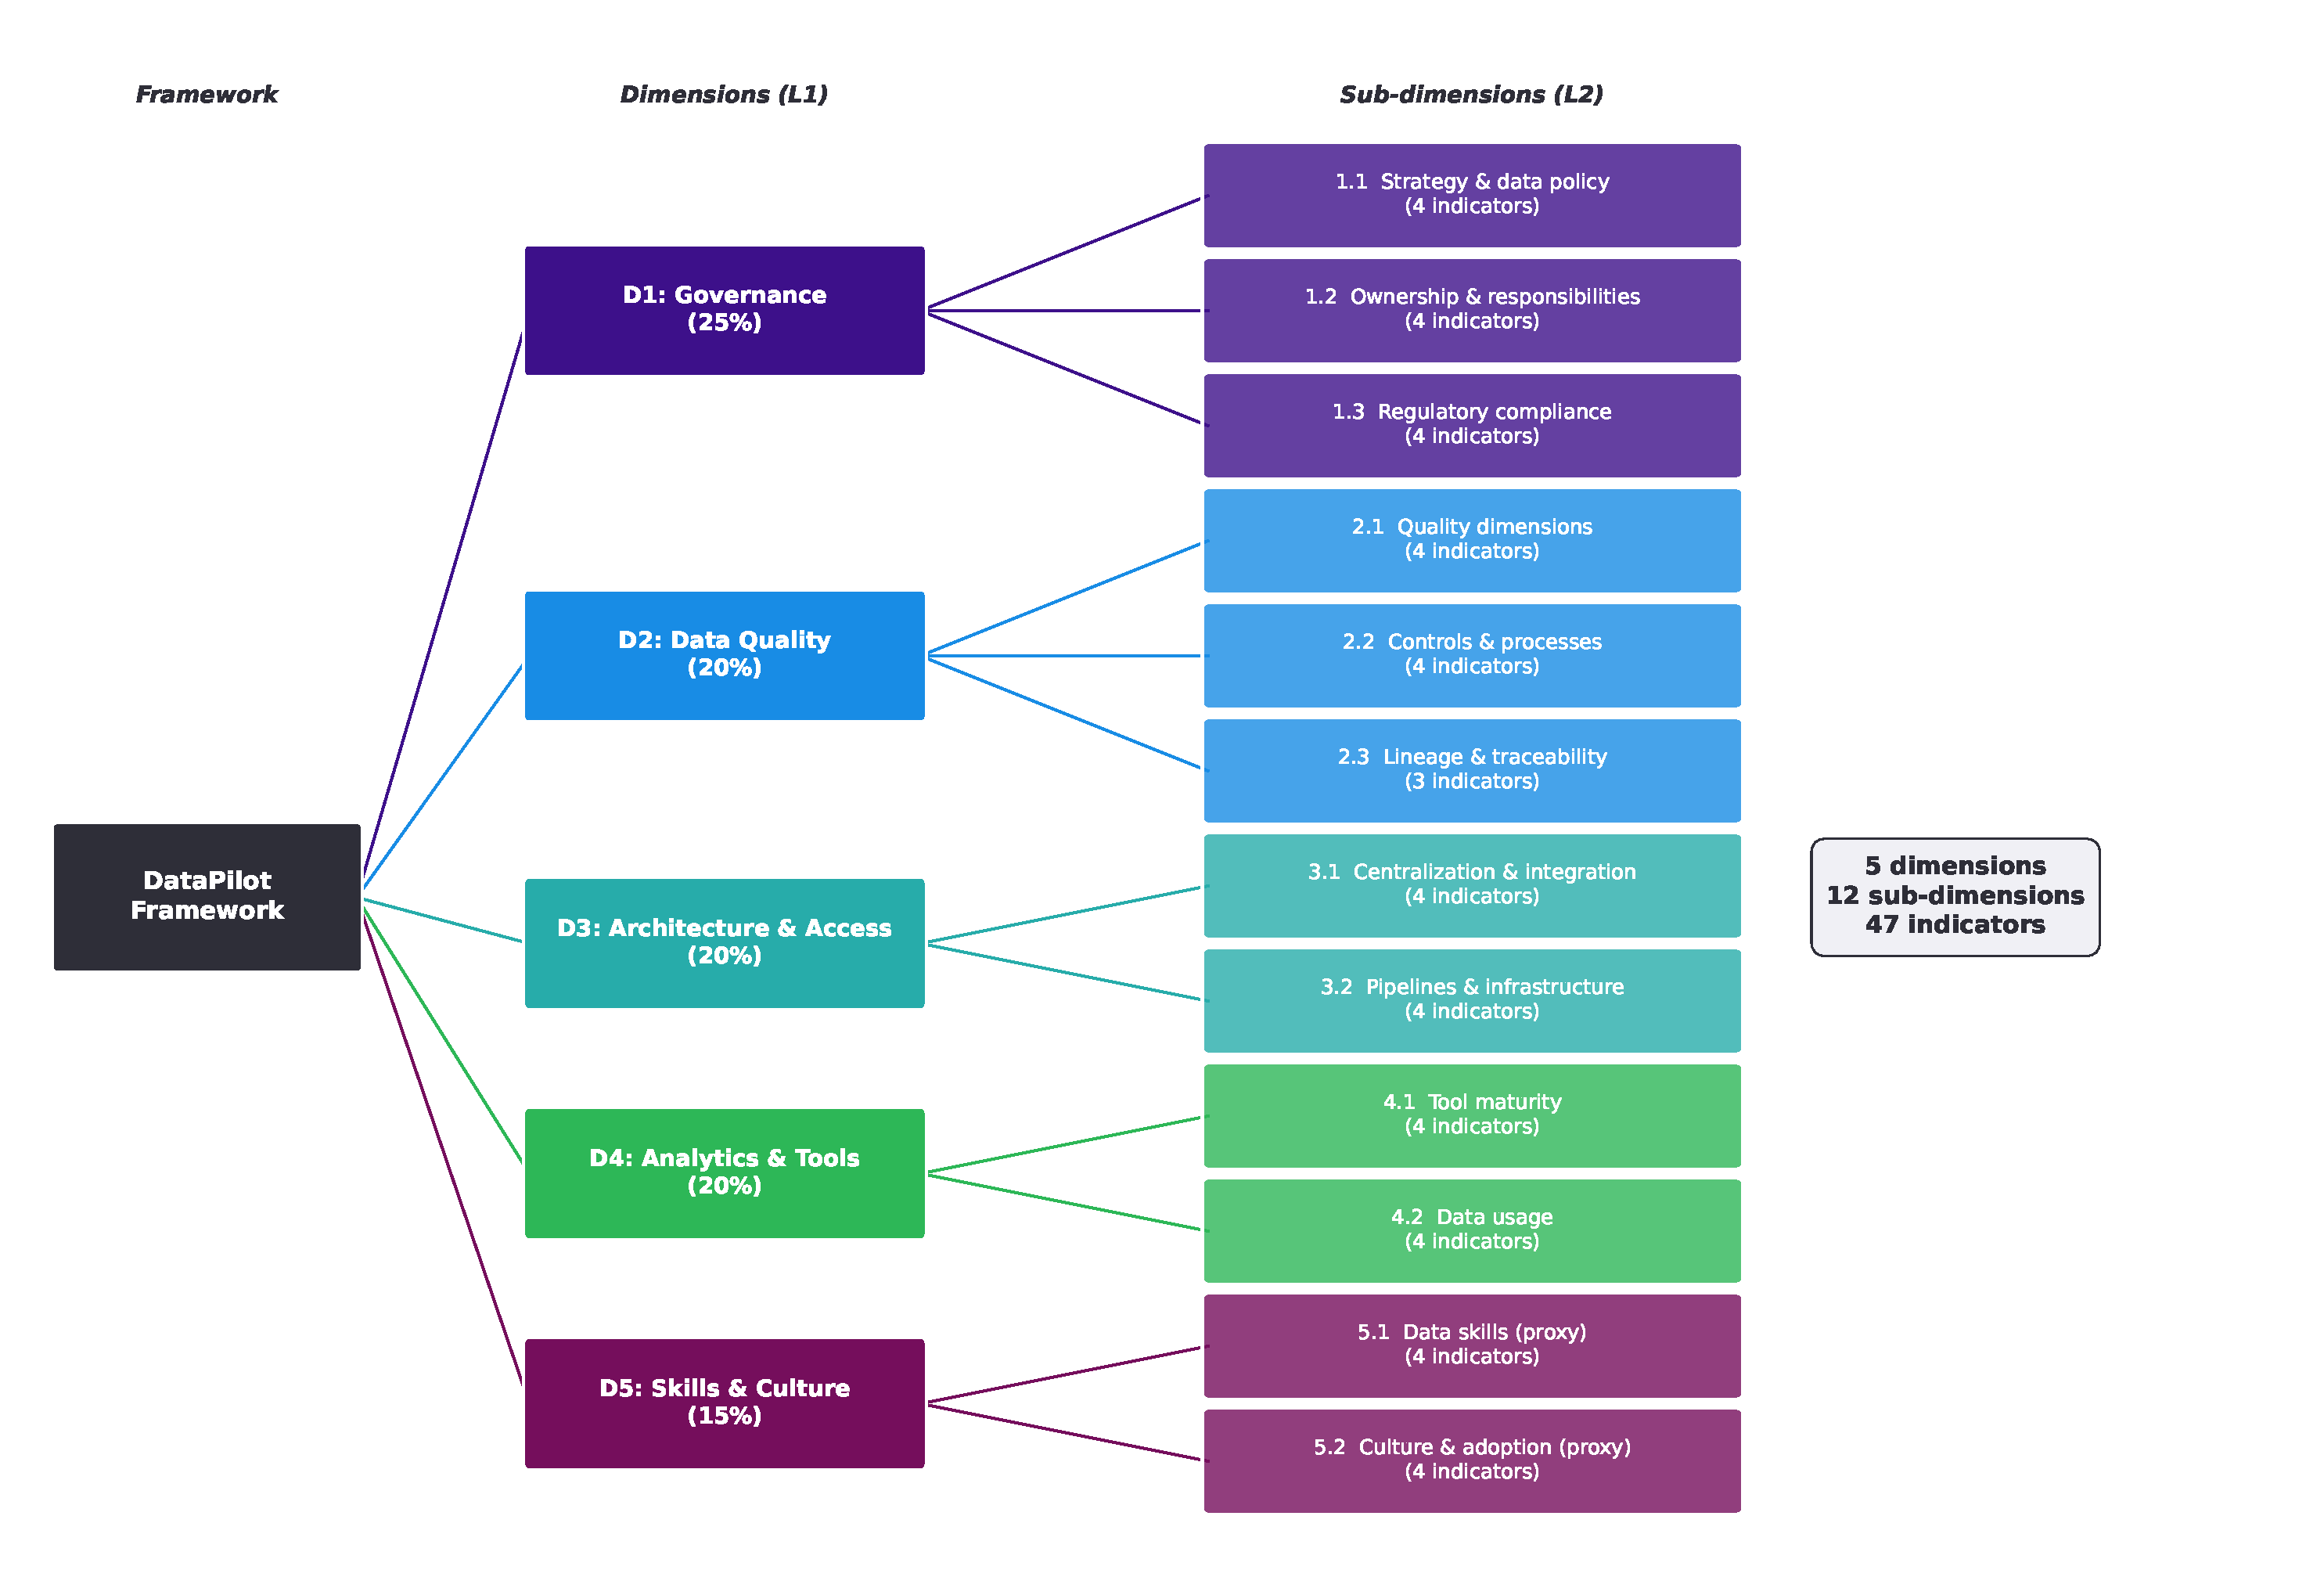
\includegraphics[width=\textwidth]{images/framework-tree.pdf}
\caption{Architecture of the data maturity framework: dimensions, sub-dimensions, and indicators}
\label{fig:framework-tree}
\end{figure}

\begin{table}[H]
\centering
\begin{tabular}{|p{4.6cm}|c|c|c|p{2.6cm}|}
\hline
\textbf{Dimension} & \textbf{Weight} & \textbf{Sub-dim.} & \textbf{Indic.} & \textbf{Primary sources} \\
\hline
D1 Governance & 25\% & 3 & 12 & DCAM, BCT \\
D2 Data Quality & 20\% & 3 & 11 & DAMA, DCAM \\
D3 Architecture and Access & 20\% & 2 & 8 & DAMA, DCAM \\
D4 Analytics and Tools & 20\% & 2 & 8 & TDWI, Gartner \\
D5 Skills and Culture & 15\% & 2 & 8 & CMMI, Gartner \\
\hline
\textbf{Total} & \textbf{100\%} & \textbf{12} & \textbf{47} & \\
\hline
\end{tabular}
\caption{The five dimensions of the framework}
\label{tab:dimensions}
\end{table}

\subsubsection{Solution Evaluation}

The framework was evaluated for coverage and applicability. It covers the five dimensions of data management without overlap, maps completely onto the regulatory requirements, and remains applicable in the sense that each indicator can be assessed from evidence available within a bank. The fifth dimension was retained as a proxy only dimension, since no direct self assessment instrument was available, a limitation recorded for the evaluation phase. The eight proxy indicators of D5 are distributed across two sub-dimensions: sub-dimension 5.1 (Data Skills) covers training program existence and budget, the headcount ratio of data professionals as a percentage of total staff, the number of data-related certifications obtained in the previous twelve months, and the number of data-specific hires in the previous twelve months; sub-dimension 5.2 (Culture and Adoption) covers the existence of a data literacy program, the presence and maturity of change management practices, the degree of business engagement with data initiatives, and the presence of communities of practice. These eight indicators can all be verified against objective and auditable evidence, which preserves the auditability property of the framework for this dimension. Having fixed what data maturity means for a Tunisian bank, the next iteration turns this structure into a measurement instrument.

\subsection{Iteration 2: The Scoring Methodology}

The second iteration turns the framework into a measurement instrument by designing an auditable scoring methodology. It follows the same five activities of the regulative cycle.

\subsubsection{Problem Investigation}

A structure of indicators, however complete, is not sufficient on its own. To be useful to bank management and defensible before a supervisor, the framework must condense the 47 indicator scores into a single figure that is comparable across institutions and over time, and that is auditable, in the sense that every number can be retraced to the evidence behind it. The second iteration therefore addresses the problem of aggregating the indicator scores into a defensible Global Maturity Index. Three difficulties make this non-trivial. First, the aggregation must combine indicators, sub-dimensions, and dimensions of unequal importance into one score without losing the meaning of the parts. Second, the score must resist over-optimistic self-assessment, since the diagnostic survey showed that institutions tend to rate themselves more advanced than their evidence supports, so an aggregation that trusts unsupported claims would produce an index that would not hold up under supervisory scrutiny. Third, the method must handle indicators that do not apply to a given institution without letting a respondent either evade the regulatory core or hollow out the index by skipping inconvenient items. A satisfactory solution must therefore be weighted, evidence-bound, robust to skipping, and traceable from the individual answer up to the global score. The aggregation model that follows is an original contribution of this work: while the five benchmark frameworks supply the dimension structure, the five-level scale, and the executive labels, none of them prescribes how indicator responses combine into a single defensible score, so the weighted, evidence-bound, renormalized chain designed here is authored rather than adopted.

\subsubsection{Solution Design}

A weighted aggregation model was designed. Each indicator is scored from one to five. A sub-dimension score is the average of the effective scores of its indicators, a dimension score is the average of its sub-dimension scores, and the global score, which is termed the Global Maturity Index (GMI), is the weighted sum of the dimension scores. To keep the index defensible when a dimension is left unanswered, the dimension weights are renormalized over the total weight of the answered dimensions only, so that the retained weights always sum to one hundred percent. For instance, if Skills and Culture (15\%) is left unanswered, the remaining 85\% is rescaled to 100\%, so Governance's 25\% becomes 25/85, about 29\%. The design also introduced four business rules. The first is the evidence requirement: every score must be supported by a verifiable artifact such as an approved document, a system log, an active dashboard, or a measured figure. The second is the evidence cap, the project's anti-gaming rule, which operationalizes a key distinction between strategy and formalization: possessing a data strategy is not sufficient, it must be documented, approved, dated, and accessible; any indicator score above two out of five for which no supporting evidence is recorded is capped at two. This rule directly addresses the perception versus reality gap observed in the survey, where institutions tend to rate themselves more advanced than their evidence supports. What the cap enforces is the presence of a cited artifact, not its authenticity: the tool requires that an artifact be named for a high score to stand, but it does not itself verify that the artifact exists, is approved, or is relevant, which remains the responsibility of the assessor and of any subsequent reviewer or auditor who can re-examine the exported evidence package. The cap therefore removes the easiest form of inflation, an unsupported high claim, without pretending to adjudicate the quality of the evidence. The third business rule is the skip logic mechanism: no more than 20\% of the indicators of a dimension may be skipped, this limit being computed as the count of indicators multiplied by 20\% and rounded down, which yields a ceiling of two skips for Governance, two for Data Quality, and one for each of Architecture and Access, Analytics and Tools, and Skills and Culture; skipped indicators are excluded from the denominator rather than scored as zero. The fourth rule is the non-skippable status of regulatory indicators: the thirteen indicators aligned with the BCT Circulaire N\textdegree{}2025-08 and BCBS 239 cannot be skipped under any circumstances. Two modeling choices underlie this aggregation and are stated explicitly. First, the five rubric levels are treated as an equal-interval scale for the purpose of averaging, a pragmatic convention that maturity indices built on CMMI-style levels commonly adopt, so that a Global Maturity Index of, for instance, 2.19 is read as a position between the Emerging and Defined levels rather than as an exact physical quantity. Second, a dimension score is the average of its sub-dimension scores rather than the average of all its indicators, which gives each sub-dimension equal weight regardless of how many indicators it contains, so that a sub-dimension's influence is not driven by its indicator count; the alternative of a single grand mean over all indicators was considered and set aside for that reason. Both are assumptions of the measurement model rather than derivations.

At a conceptual level, this design turns each indicator answer into the global score through a chain of averages and one weighted, renormalized sum. The chain, from an individual indicator score up to the global maturity level, is illustrated in Figure~\ref{fig:scoring-flow}: the effective score of each indicator feeds the average of its sub-dimension, the sub-dimension scores feed the average of their dimension, and the dimension scores feed the weighted Global Maturity Index, with the evidence cap and the skip rules acting on the individual answers and the renormalization acting on the final sum.

\begin{figure}[H]
\centering
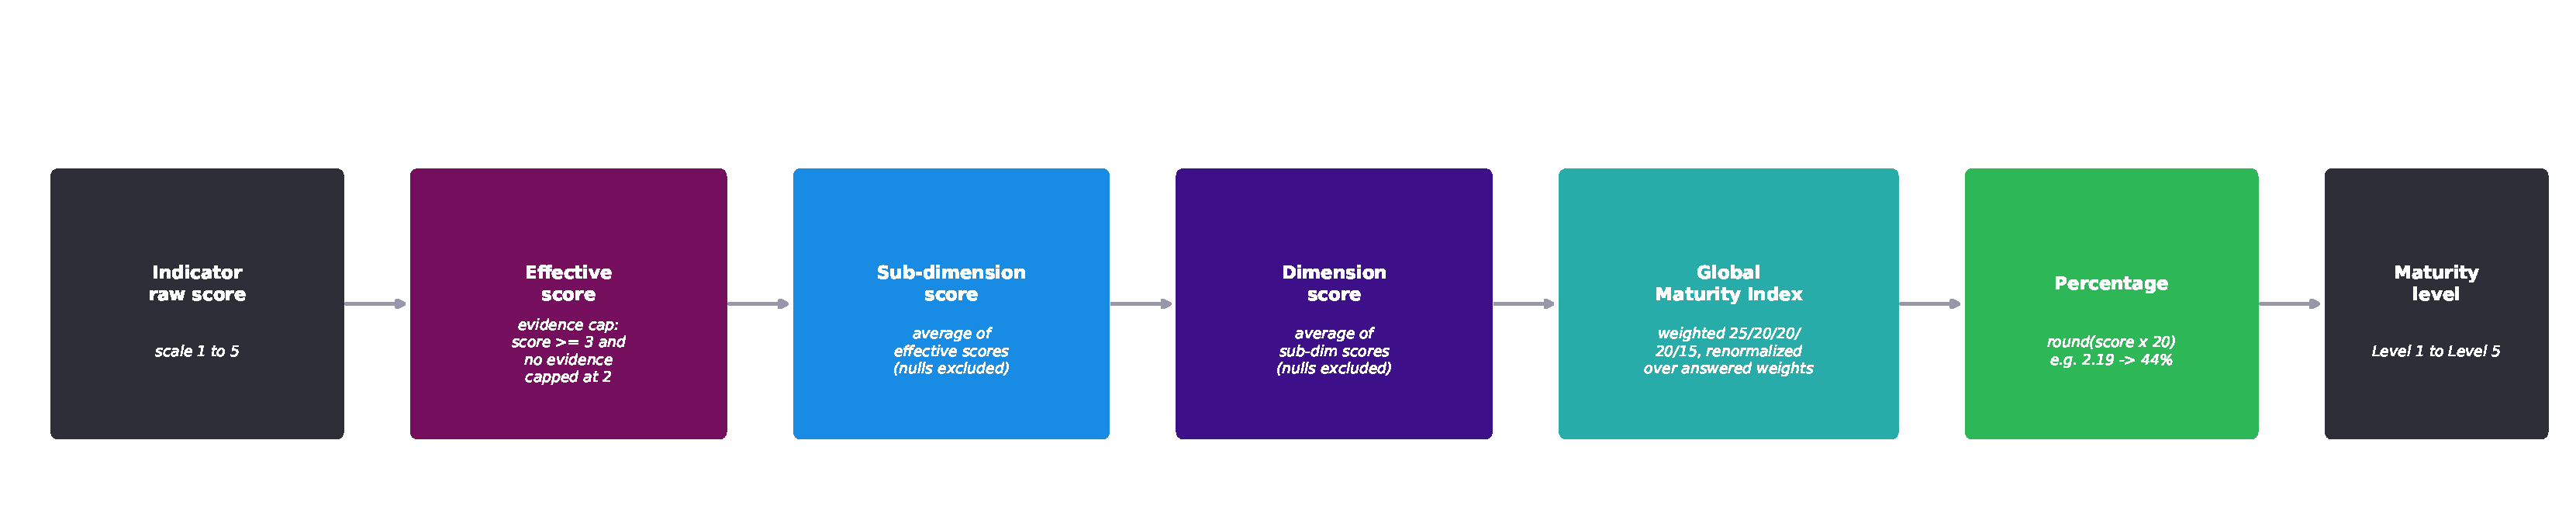
\includegraphics[width=\textwidth]{images/scoring-flow.pdf}
\caption{Score aggregation from indicators to the global maturity level}
\label{fig:scoring-flow}
\end{figure}

\subsubsection{Design Validation}

Two design risks were assessed before the engine was built. The first is score inflation: a respondent can claim a four or a five that no artifact supports, and an aggregation that accepts such claims produces an index that would not withstand supervisory scrutiny. The design forecloses this case by construction, since the evidence cap computes any score above two without a documented artifact as a two before any averaging occurs, so an unsupported claim can never raise a sub-dimension, a dimension, or the global index above the level the evidence sustains. The second risk is denominator distortion: a respondent could reshape a dimension score by skipping its inconvenient indicators, or hollow out the index by leaving a whole dimension unanswered.

The worst case combining both risks was traced through the rules on paper before implementation. Consider Governance driven to its skip ceiling of two, so that ten of its twelve indicators remain in the denominator, with one of the remaining indicators claimed at four out of five and an empty evidence field. The cap turns the four into an effective two before the sub-dimension average is formed; the two skipped indicators leave the denominator rather than entering it as zeros, so the omission neither inflates nor deflates the average; and the resulting dimension score enters the weighted sum with its nominal 25\% weight. If the same respondent then leaves an entire dimension unanswered, the renormalization rule rescales the weights of the answered dimensions so that they again sum to one hundred percent, and the Global Maturity Index remains defined and comparable instead of silently losing part of its weight. Finally, the thirteen regulatory indicators cannot be skipped at all, so the regulatory core of the assessment can never be evaded through either mechanism. The concrete instrument of this validation was the worked recomputation of the aggregation chain, which confirmed that a change in an indicator propagates correctly through its sub-dimension and dimension to the global score and that the weighting sums to one hundred percent in every configuration. The business rules were validated against the requirement of auditability: every score must be traceable to documented evidence.

\subsubsection{Solution Implementation}

A rigorous scoring methodology is necessary because qualitative assessments without a score produce subjective and incomparable results. A numeric score forces documentary evidence, enables cross-bank benchmarking over time, is built so that a supervisory audit could succeed by retracing every figure to the evidence behind it, and gives management a clear and actionable figure to track. The Global Maturity Index (GMI) is computed as a weighted sum of the five dimension scores, renormalized over the weights of the answered dimensions, and is then converted into a percentage by multiplying by twenty and rounding to the nearest integer. When every dimension is answered, the renormalized weights coincide with the nominal weights and the index takes the following form:

\begin{equation}
\text{GMI} = 0.25\,D_1 + 0.20\,D_2 + 0.20\,D_3 + 0.20\,D_4 + 0.15\,D_5
\end{equation}

Where the conceptual chain of Figure~\ref{fig:scoring-flow} showed the design of the aggregation, the implementation view traces what the engine actually does with a single response at runtime, including the decisions it takes on the way. A raw response, consisting of a score from one to five together with an optional evidence text and a skipped flag, first passes through the effective score computation, which decides whether to exclude the indicator (skipped or unanswered), to cap its score at two (three or more without evidence), or to keep it as entered. The surviving effective scores are then averaged within each sub-dimension, the sub-dimension scores within each dimension, and the dimension scores combined by the renormalized weighted sum that yields the Global Maturity Index, from which the percentage and the maturity level are derived. This runtime processing is shown as an activity in Figure~\ref{fig:data-flow}, which makes explicit where each business rule intervenes: the evidence cap and the skip and non-skippable rules act on the individual response, while renormalization acts at the final aggregation step.

\begin{figure}[H]
\centering
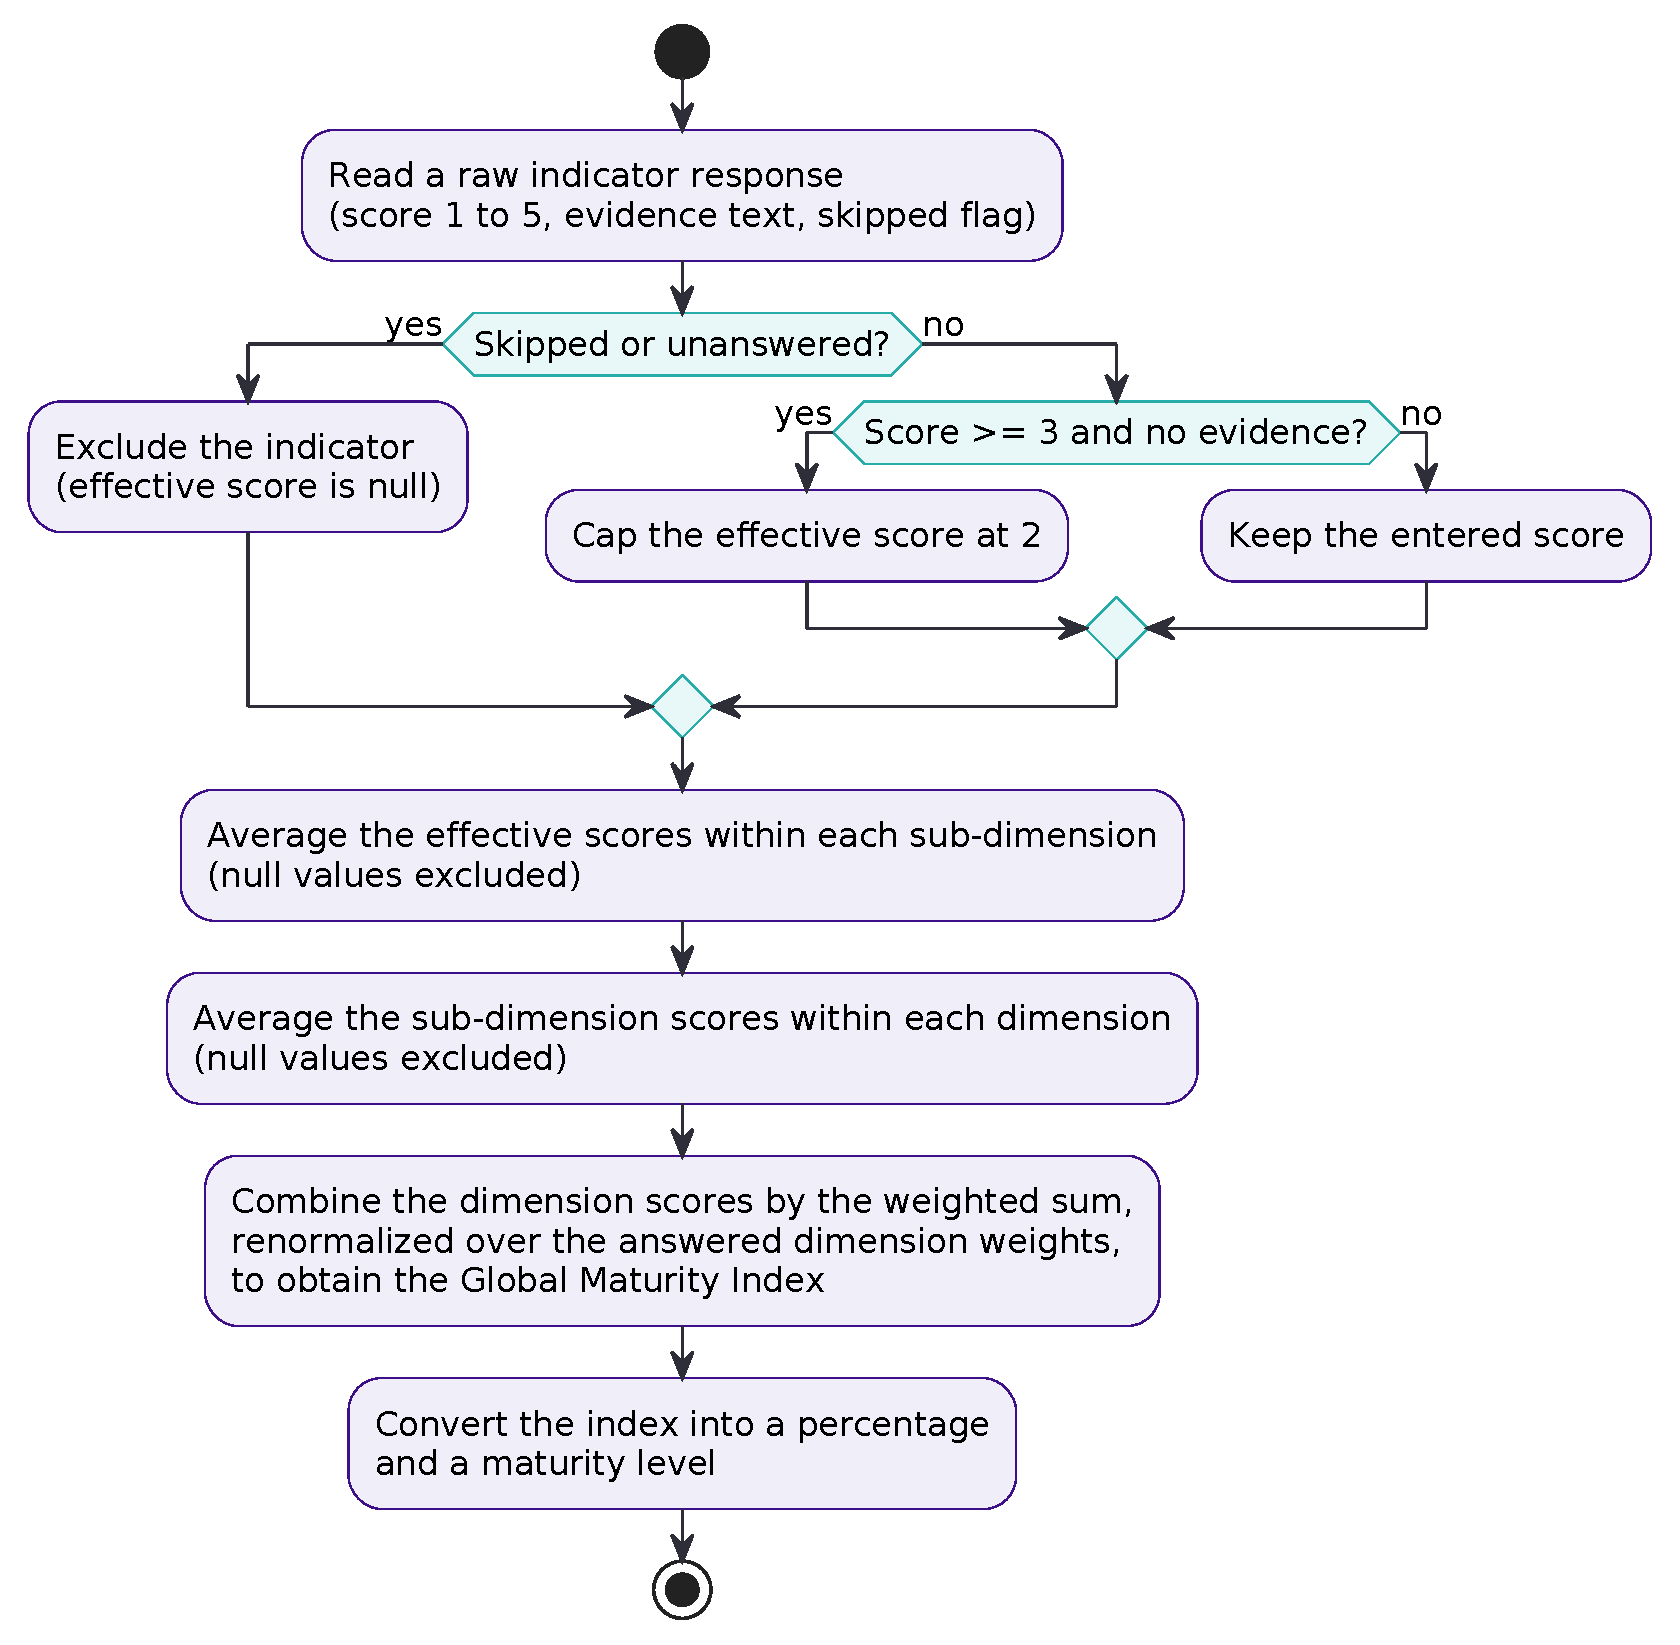
\includegraphics[width=0.9\textwidth]{images/data-flow.pdf}
\caption{Data flow through the scoring engine, from indicator responses to the Global Maturity Index}
\label{fig:data-flow}
\end{figure}

The Global Maturity Index, a continuous value on the one to five scale, is mapped to one of five discrete maturity levels by equal bands: Level~1 (Initial) from 1.00 to 1.79, Level~2 (Emerging) from 1.80 to 2.59, Level~3 (Defined) from 2.60 to 3.39, Level~4 (Managed) from 3.40 to 4.19, and Level~5 (Optimized) from 4.20 to 5.00. A GMI of 2.19, for instance, falls in the second band and is therefore reported as Level~2, Emerging. The levels are reported on this five level scale derived from CMMI, complemented by the Gartner labels, as summarized in Table~\ref{tab:maturity-levels}.

\begin{table}[H]
\centering
\begin{tabular}{|c|l|l|}
\hline
\textbf{Level} & \textbf{CMMI Name} & \textbf{Gartner Label} \\
\hline
1 & Initial (ad hoc) & Unaware \\
2 & Emerging (partial, informal) & Aware \\
3 & Defined (formalized, standardized) & Active \\
4 & Managed (quantitative monitoring) & Effective \\
5 & Optimized (systemic innovation) & Transformative \\
\hline
\end{tabular}
\caption{Maturity levels and their executive labels}
\label{tab:maturity-levels}
\end{table}

The five maturity levels and their executive labels are illustrated as an ascending progression in Figure~\ref{fig:maturity-ladder}.

\begin{figure}[H]
\centering
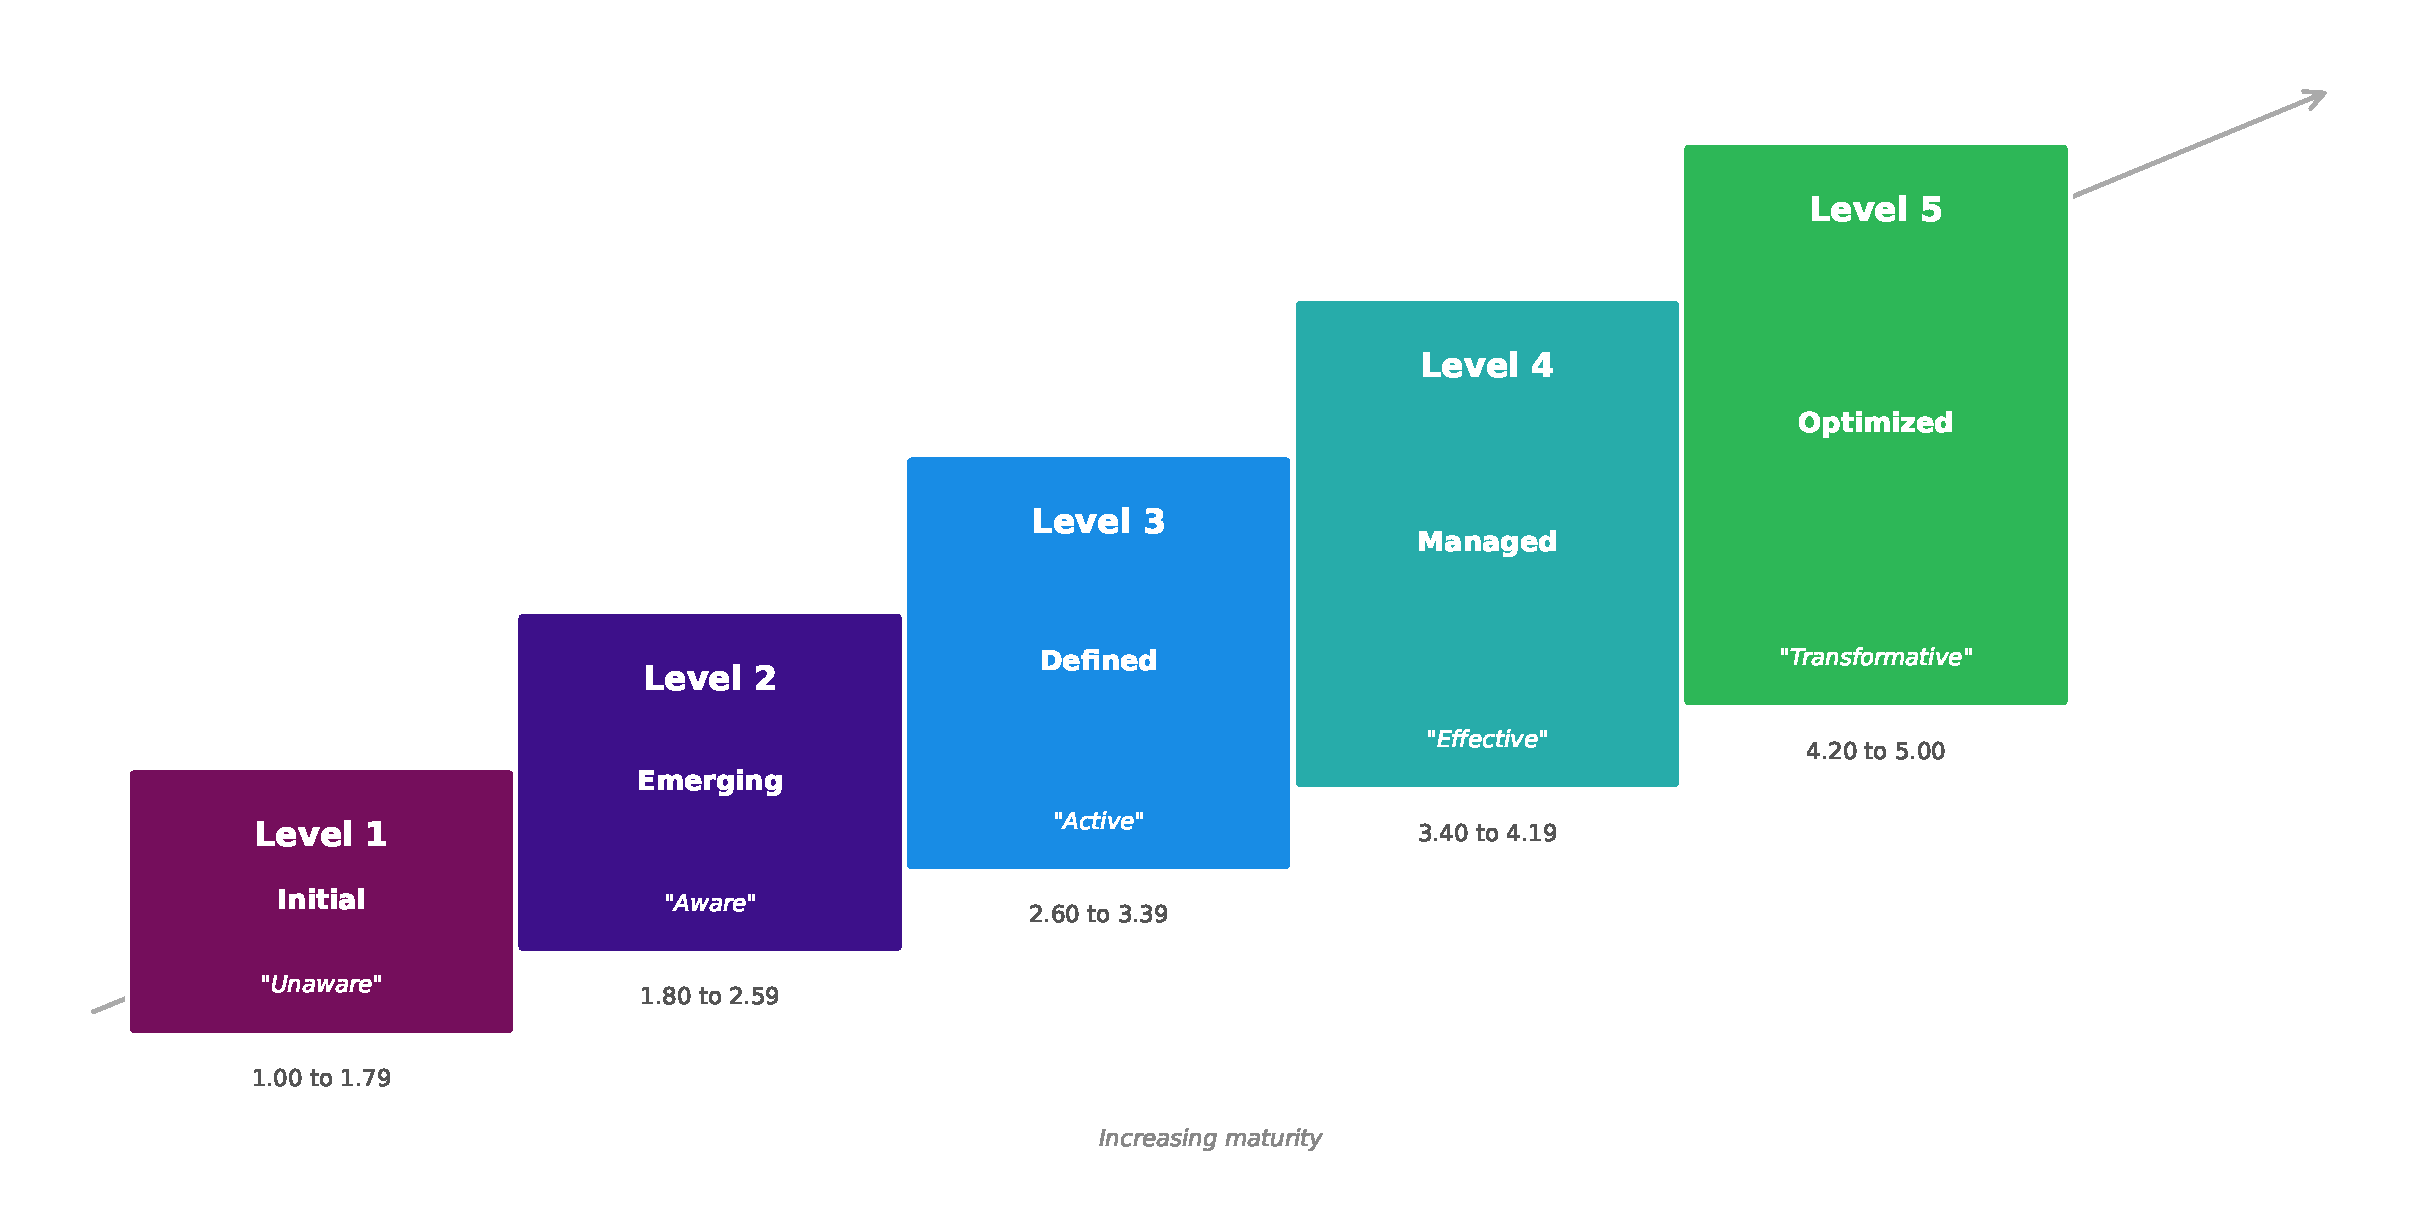
\includegraphics[width=0.8\textwidth]{images/maturity-ladder.pdf}
\caption{The five maturity levels and their executive labels}
\label{fig:maturity-ladder}
\end{figure}

\begin{sloppypar}
The aggregation chain is implemented in the application state module \texttt{src/store/useAppStore.js}, where the selectors \texttt{getEffectiveScore}, \texttt{getSubDimScore}, \texttt{getDimScore}, \texttt{getGlobalScore}, and \texttt{getPercentage} compute, respectively, the evidence-adjusted score of a single indicator, the average of the effective scores of a sub-dimension, the average of the sub-dimension scores of a dimension, the weighted global score renormalized over the answered dimension weights, and its conversion into a percentage as the score multiplied by twenty and rounded.
\end{sloppypar}

The four business rules of the solution design are enforced directly in the code: the selector \texttt{getEffectiveScore} applies the evidence cap before any aggregation, and the \texttt{skipIndicator} action refuses both to skip a regulatory indicator and to exceed the skip limit of a dimension, computed as 20\% of its indicators rounded down. A one-page summary of all the scoring rules, from the evidence cap through the maturity bands to the compliance thresholds, is provided in Appendix~E.

The possible states of a single indicator under these rules are modelled in Figure~\ref{fig:state}. In that figure, and wherever a skipped or unanswered indicator is shown to carry a null effective score, ``null'' means that the indicator is excluded from the average of its sub-dimension, not that it is counted as a zero; scoring an omitted indicator as zero would penalise a bank for an item that does not apply and would defeat the anti-gaming purpose of the skip rule, which is precisely why skipped indicators leave the denominator rather than entering it as zeros.

\begin{figure}[H]
\centering
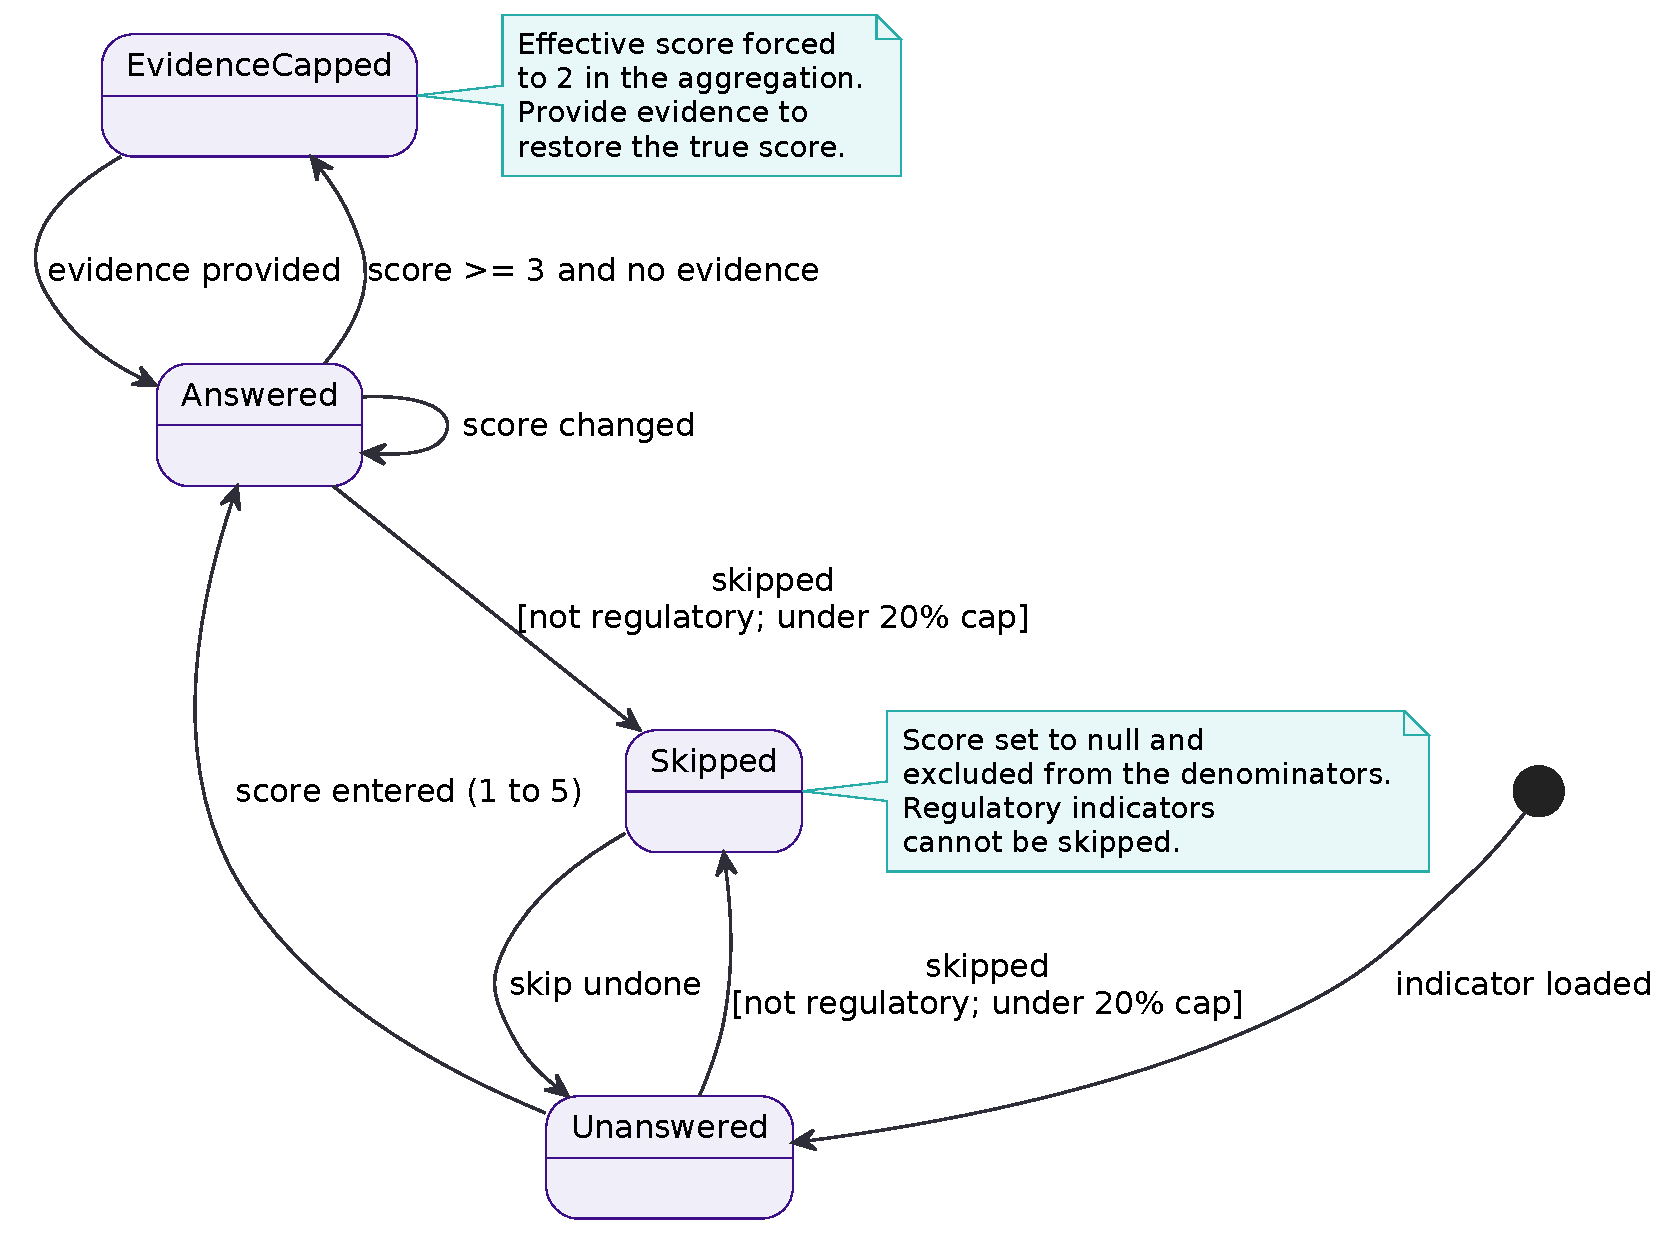
\includegraphics[width=0.65\textwidth]{images/indicator-state.pdf}
\caption{States of an indicator under the scoring rules}
\label{fig:state}
\end{figure}

The interaction between the analyst and the scoring engine, for the solo assessment scenario, is best read in two parts. The first part, in Figure~\ref{fig:sequence-capture}, is the capture of a single answer: the analyst enters a score and its evidence on the questionnaire screen, and the engine records them and persists the work in progress. The second part, in Figure~\ref{fig:sequence-aggregate}, is the aggregation performed when the analyst opens the Results screen: the engine computes the effective scores, averages them up the hierarchy, and returns the Global Maturity Index and its derived values for display.

\begin{figure}[H]
\centering
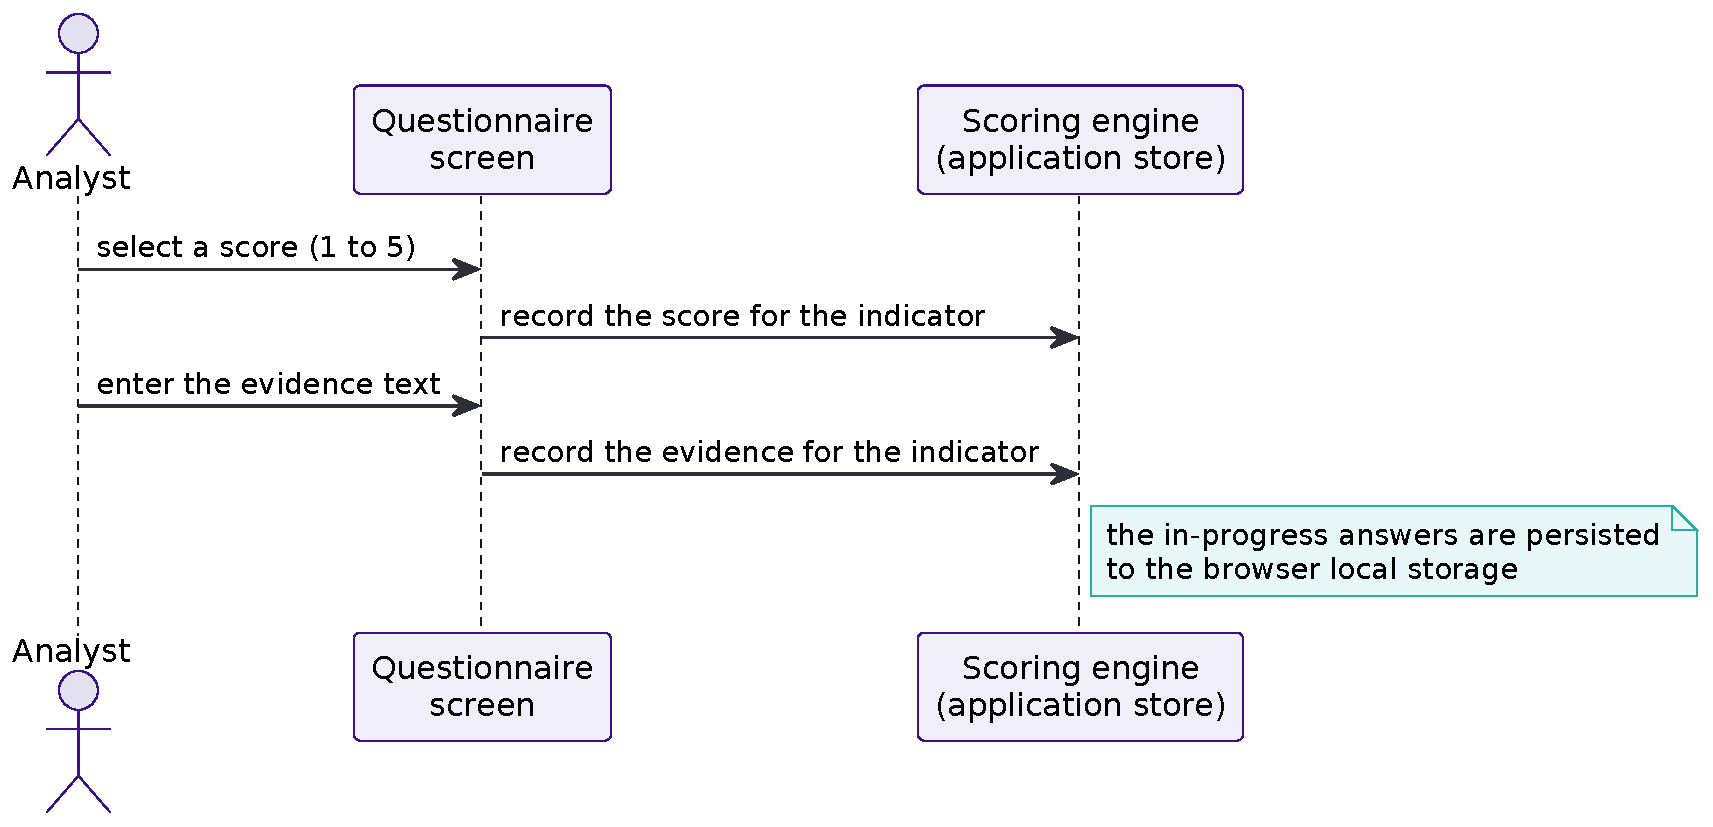
\includegraphics[width=0.85\textwidth]{images/sequence-scoring-capture.pdf}
\caption{Sequence diagram of capturing an indicator answer in a solo assessment}
\label{fig:sequence-capture}
\end{figure}

\begin{figure}[H]
\centering
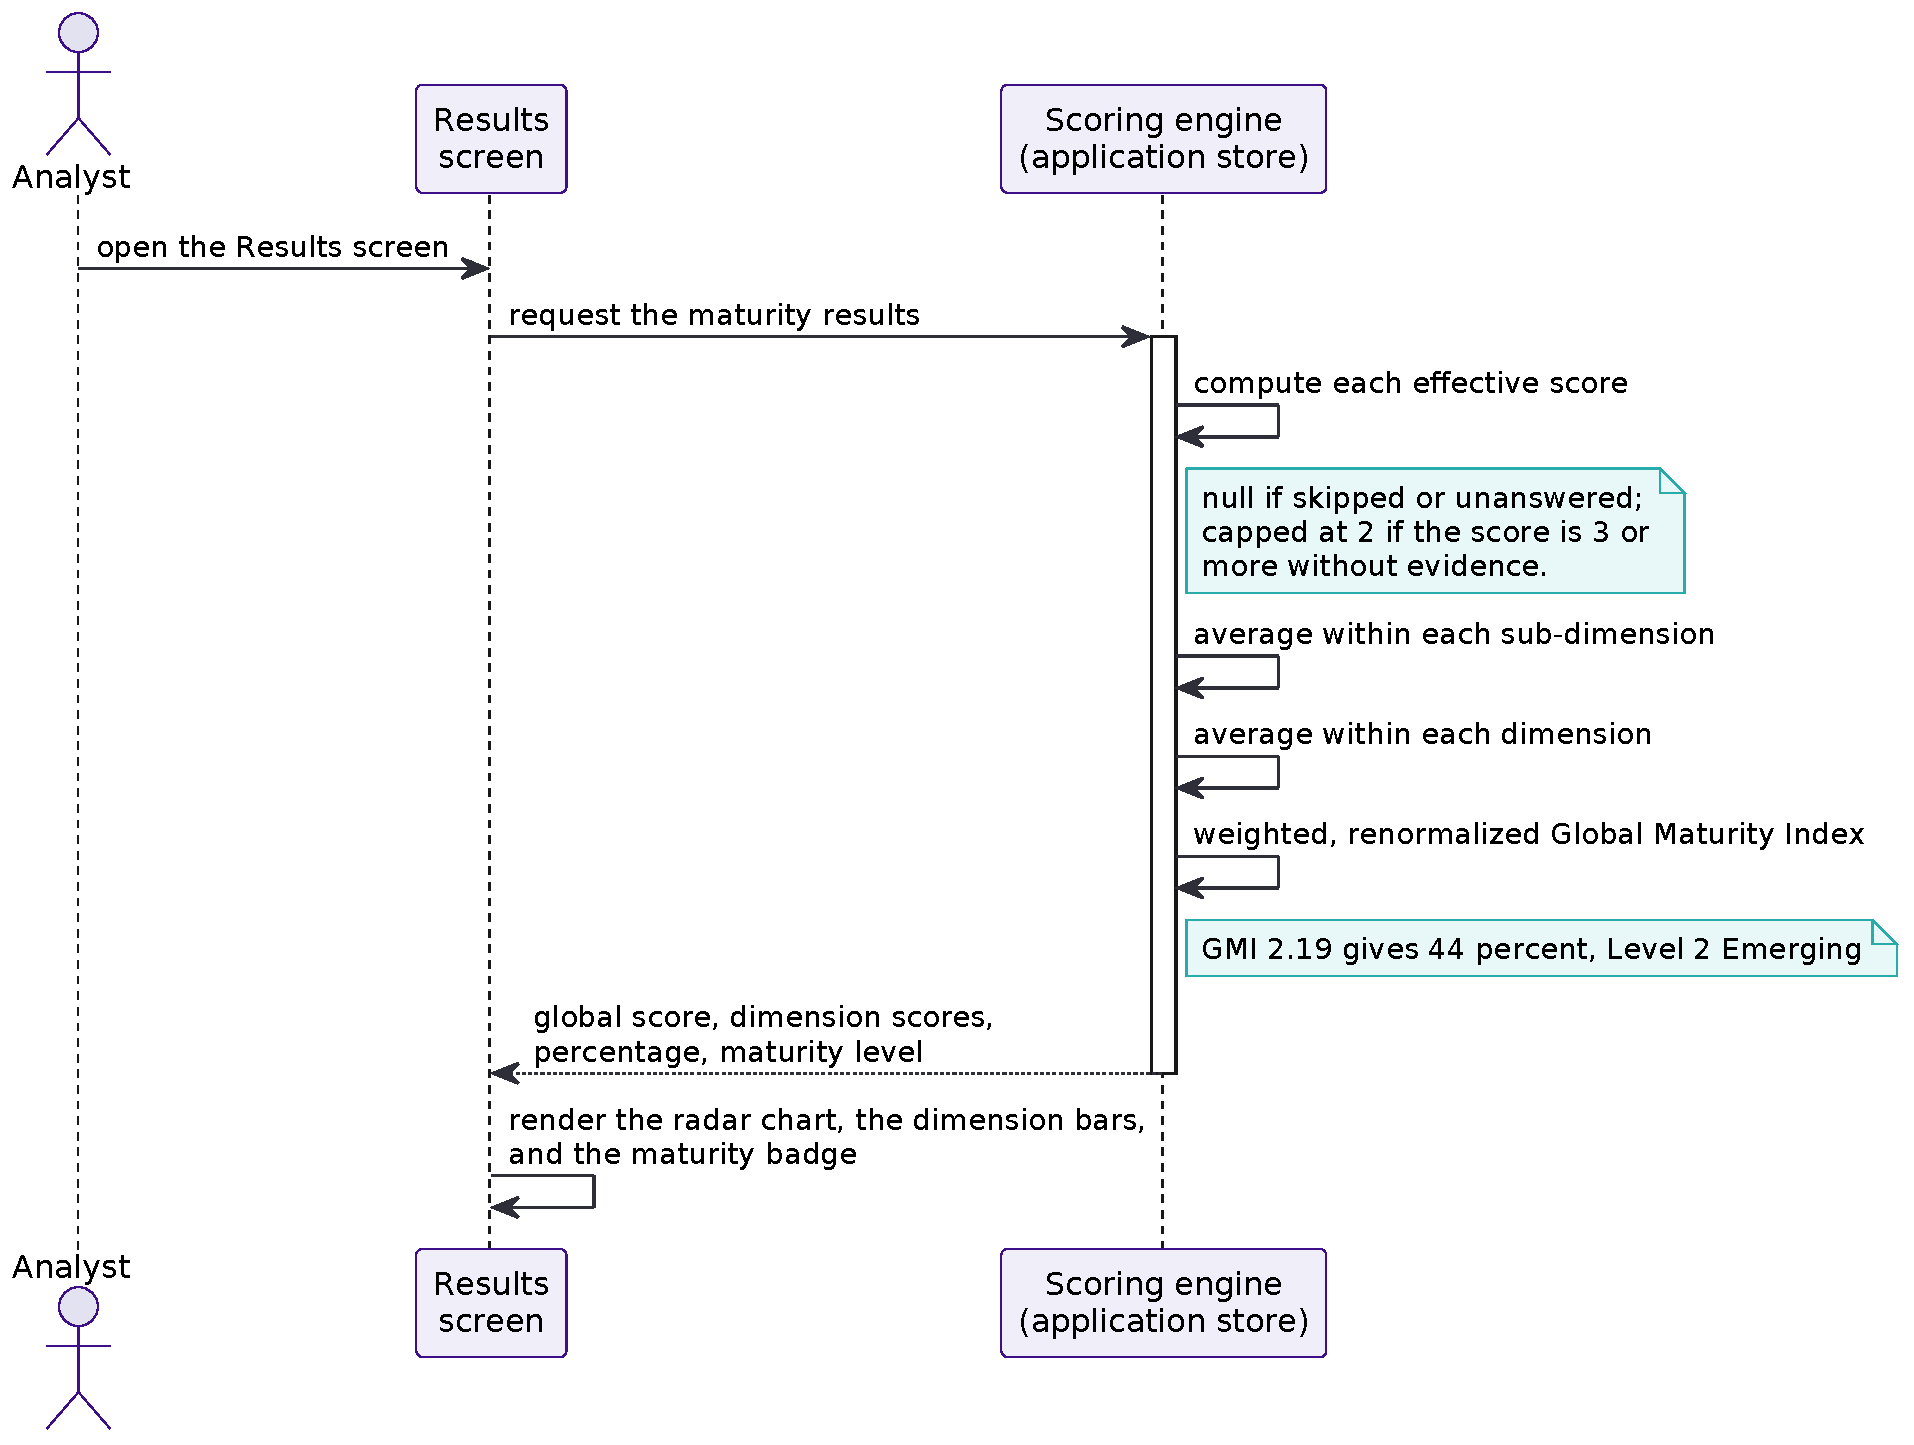
\includegraphics[width=0.9\textwidth]{images/sequence-scoring-aggregate.pdf}
\caption{Sequence diagram of aggregating the scores on the Results screen in a solo assessment}
\label{fig:sequence-aggregate}
\end{figure}

\subsubsection{Solution Evaluation}

The scoring methodology was evaluated on a worked example, an illustrative figure chosen to exercise the aggregation chain rather than a measurement of any real bank: a Global Maturity Index of 2.19 out of 5 corresponds to 44\%, which places the institution at Level 2, Emerging (Gartner label: Aware). The example confirmed that the aggregation chain, the percentage conversion, and the level mapping behave consistently, and that the business rules produce an auditable result. The evidence cap was verified to function correctly: an indicator rated four out of five without supporting documentation is computed as two, which reduces the effective dimension score and prevents score inflation. Having made the measurement auditable, the next iteration embeds the engine in the tool through which a bank actually operates it.

\subsection{Iteration 3: The DataPilot Tool}

The third iteration operationalizes the framework and its scoring methodology in an interactive tool, DataPilot, usable by a single assessor. It proceeds once more through the five activities of the regulative cycle.

\subsubsection{Problem Investigation}

For the framework and its scoring methodology to be usable by bank management, they must be embedded in an accessible tool that automates the computation and presents the results clearly. The third iteration addresses the problem of operationalizing the framework as an interactive application; at this stage of the project, the tool targets a single assessor operating it locally.

\subsubsection{Solution Design}

\begin{sloppypar}
DataPilot was designed around six screens, Welcome, Profile, Questionnaire, Results, Gap Analysis, and Compliance, and structured as a layered front end. The screens are implemented as page components in the \texttt{src/pages} directory, supported by shared layout components such as the navigation bar and the progress bar, and by reusable interface elements such as the score and maturity badges, grouped in \texttt{src/components}; the charts are isolated in \texttt{src/charts}. At this stage of the project the content of the framework was stored as a structured data module rather than an external database, a choice that Iteration 4 later revisits by moving the content into per-bank data seeded from the EY master template: \texttt{src/data/indicators.js} declares the five dimensions with their weights, the twelve sub-dimensions, and the 47 indicators, each carrying its identifier, its dimension and sub-dimension, a regulatory flag marking the thirteen indicators derived from the regulatory requirements, the question, a guidance hint, and a five level scoring rubric, while \texttt{src/data/recommendations.js} stores the improvement actions proposed for each dimension at three maturity bands. The application state is held in a single Zustand store, \texttt{src/store/useAppStore.js}, which records the institution profile, the answers as a map from each indicator identifier to a score, an evidence text, and a skipped flag, and the target maturity level; the same store exposes the scoring selectors of Iteration 2 and persists the assessment to the browser local storage under the key \texttt{datapilot-assessment} so that work in progress survives page reloads. The regulatory compliance mapping is carried by the regulatory flag of each indicator, from which the selector \texttt{getBCTCompliance} derives the number of compliant, non compliant, and pending regulatory indicators, an overall compliance rate, and a resulting exposure level. The questionnaire collects the indicator scores with their rubrics and hints, the scoring engine applies the aggregation logic and business rules automatically, the Results dashboard presents the maturity profile, the Gap Analysis screen prioritizes improvement actions, and the Compliance screen maps the indicators to the regulatory requirements.
\end{sloppypar}

The end-to-end journey that a single assessor follows through these six screens, from the Welcome screen to the printable export, is shown in Figure~\ref{fig:user-journey}.

\begin{figure}[H]
\centering
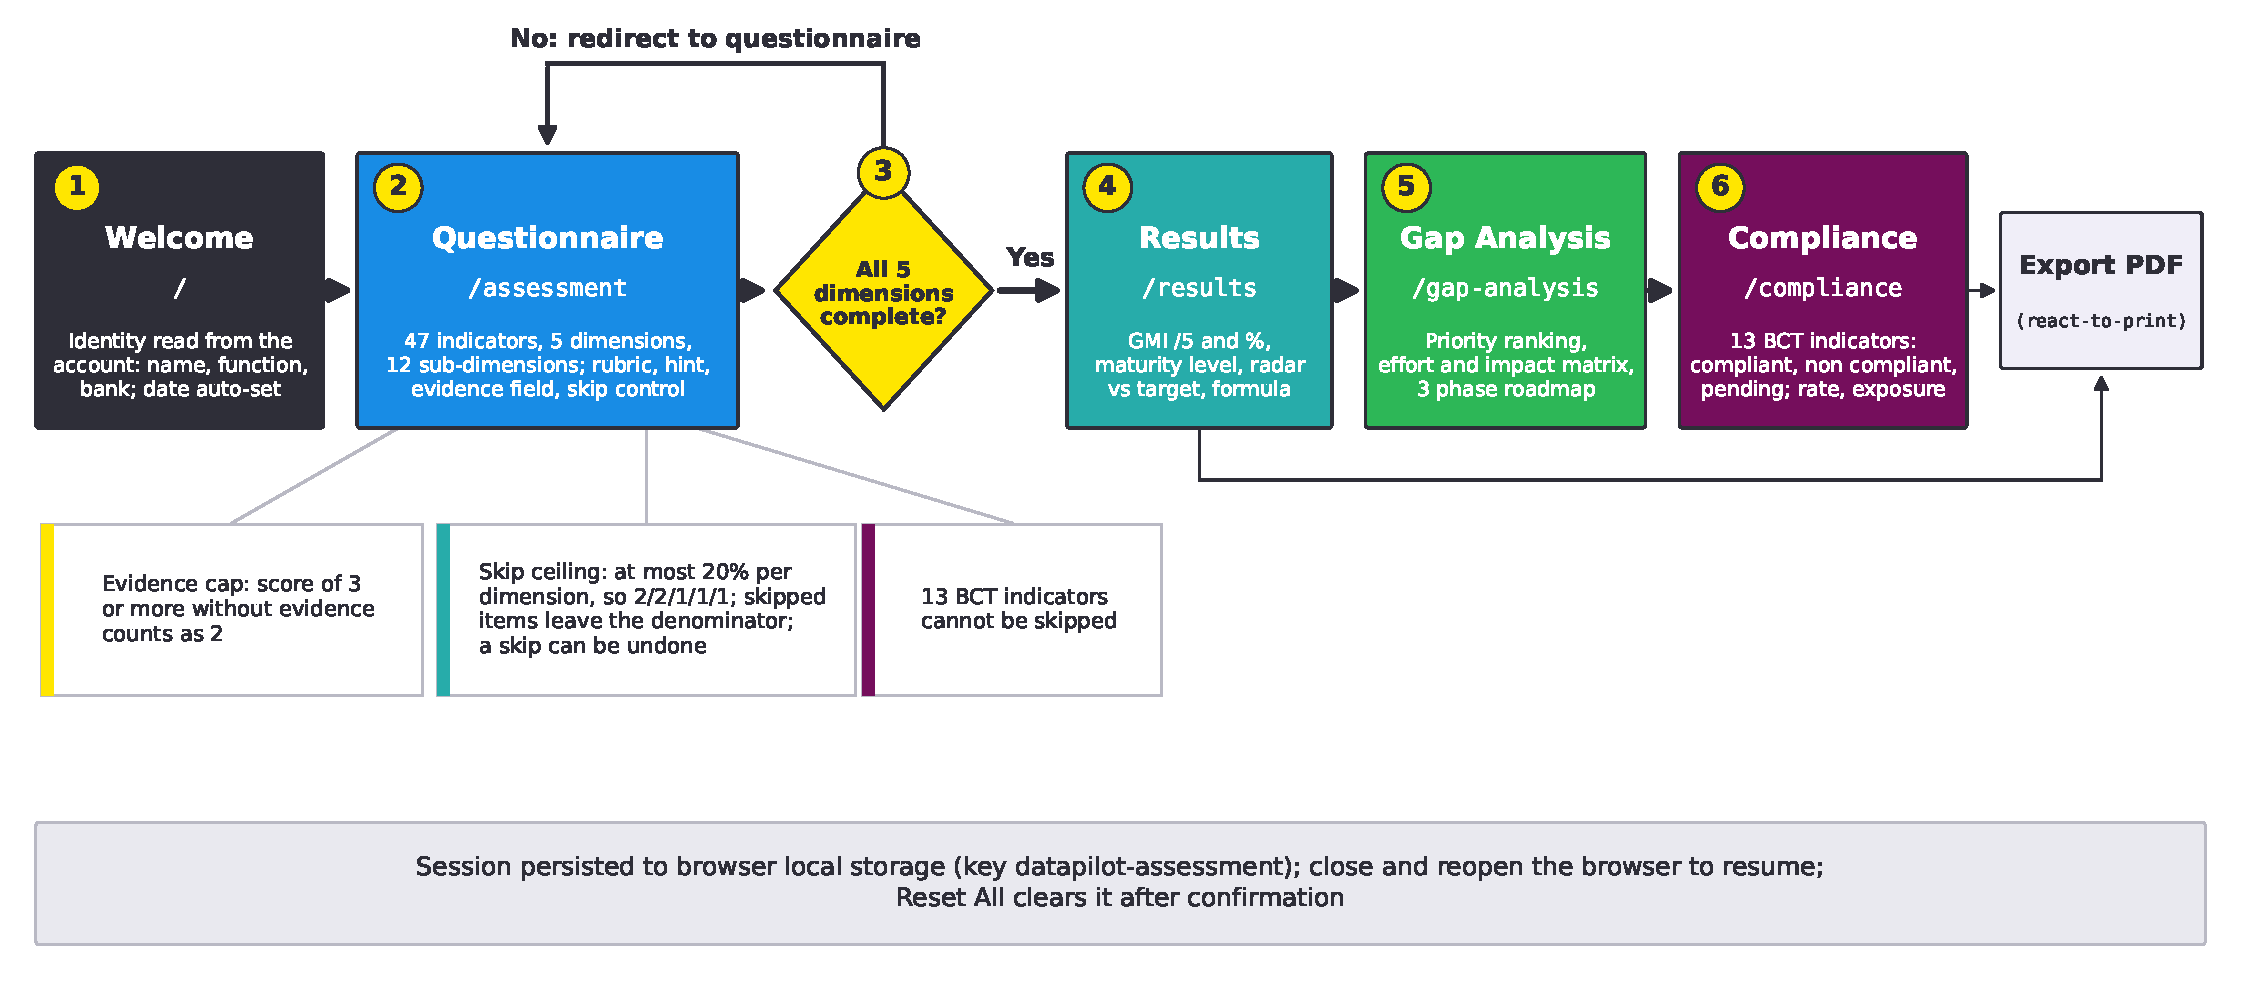
\includegraphics[width=\textwidth]{images/user-journey.pdf}
\caption{End to end user journey through DataPilot, from the Welcome screen to the printable export}
\label{fig:user-journey}
\end{figure}

Three cross-cutting views of the design, its layered architecture, its domain model, and its deployment, are described here in their Iteration~3 form and then shown as consolidated figures in Iteration~4, where the backend layer, the platform entities, and the production deployment complete each view; presenting each once, in its final form, avoids drawing three diagrams twice. The design of DataPilot follows a layered architecture, which can be read as a set of horizontal layers. At the top sat a presentation layer, formed by the six page components in \texttt{src/pages} together with the shared layout components, the navigation bar and the progress bar in \texttt{src/components/layout}, and the reusable interface elements such as the score, maturity, and regulatory badges in \texttt{src/components/ui}. Below it sat a visualization layer, the radar chart and the dimension bars isolated in \texttt{src/charts}, which the presentation layer consumed but did not implement directly. Beneath these sat a state and logic layer, the single Zustand store in \texttt{src/store/useAppStore.js}, which held the assessment state and exposed every scoring selector and business rule of Iteration 2, and which the presentation and visualization layers read from. At the base sat a data and persistence layer, the static content modules \texttt{src/data/indicators.js} and \texttt{src/data/recommendations.js}, and the browser local storage that persisted the assessment under the key \texttt{datapilot-assessment}. This layering kept the scoring logic in one place, isolated the framework content as declarative data, and let the presentation layer remain a thin projection of the store. Iteration 4 extends this stack with a backend layer, and the resulting layered structure is shown in Figure~\ref{fig:architecture-layers}.

The data that the store manipulates had, at this stage, a small and stable domain model. An assessment was described by a profile, holding the bank name, the date, the respondent name, and the role, and by a target maturity level. The framework content was described by dimensions, each carrying a name, a weight, a color, and its list of sub-dimensions; by sub-dimensions, each carrying a name; and by indicators, each carrying an identifier, its dimension and sub-dimension, a regulatory flag, a question, a hint, and a five level rubric. The respondent contribution was described by answers, one per indicator, each holding a score, an evidence text, and a skipped flag. Because the framework content was declared as static data rather than stored in a database, the model was realized as JavaScript modules and a Zustand state object rather than as persistent database tables. Iteration 4 extends this domain model with the platform entities described later in this chapter.

At this stage of the project DataPilot was deployed as a client-side single-page application: it was built by Vite into static assets that a browser loaded once and then ran entirely on the client, with the assessment persisted to the browser local storage and no server-side component or external database involved. The absence of any server was a deliberate choice for the single-assessor milestone, keeping a bank's assessment data on the assessor's own machine, which suited the confidentiality expectations of a regulatory self assessment. Iteration 4 replaces this custody argument with tenant isolation enforced in the database---a tenant here is a single bank, and isolation means that one bank can never see another bank's data---and the deployment view of the resulting platform is shown in Figure~\ref{fig:deployment}.

\subsubsection{Design Validation}

The design was validated against the requirements of automation, in that the scoring engine reproduces the methodology of Iteration 2 exactly, and of usability, in that the navigation enforces a complete assessment before producing a result. A completion gate prevents access to the results until all five dimensions have been answered.

The completion gate itself was validated before build by walking its branches on paper. When the results route is requested, the questionnaire can stand in one of three states. If every dimension is complete, each indicator either answered or legitimately skipped, the gate opens and the dashboards render. If any dimension is incomplete, the gate redirects to the questionnaire, so a partial index can never be displayed as if it were a result. And if a respondent attempts to force completion by skipping past a dimension ceiling or by skipping a regulatory indicator, the skip action itself is refused upstream of the gate, so the dimension remains incomplete and the gate remains closed rather than opening on a hollowed out denominator. Every branch therefore ends in an explicit and recoverable state, and no path allows the tool to present a score that the methodology of Iteration 2 would not defend.

The user flow through the six screens, including the completion gate that prevents access to the dashboards before the questionnaire is finished, is shown in Figure~\ref{fig:activity}.

\begin{sidewaysfigure}
\centering
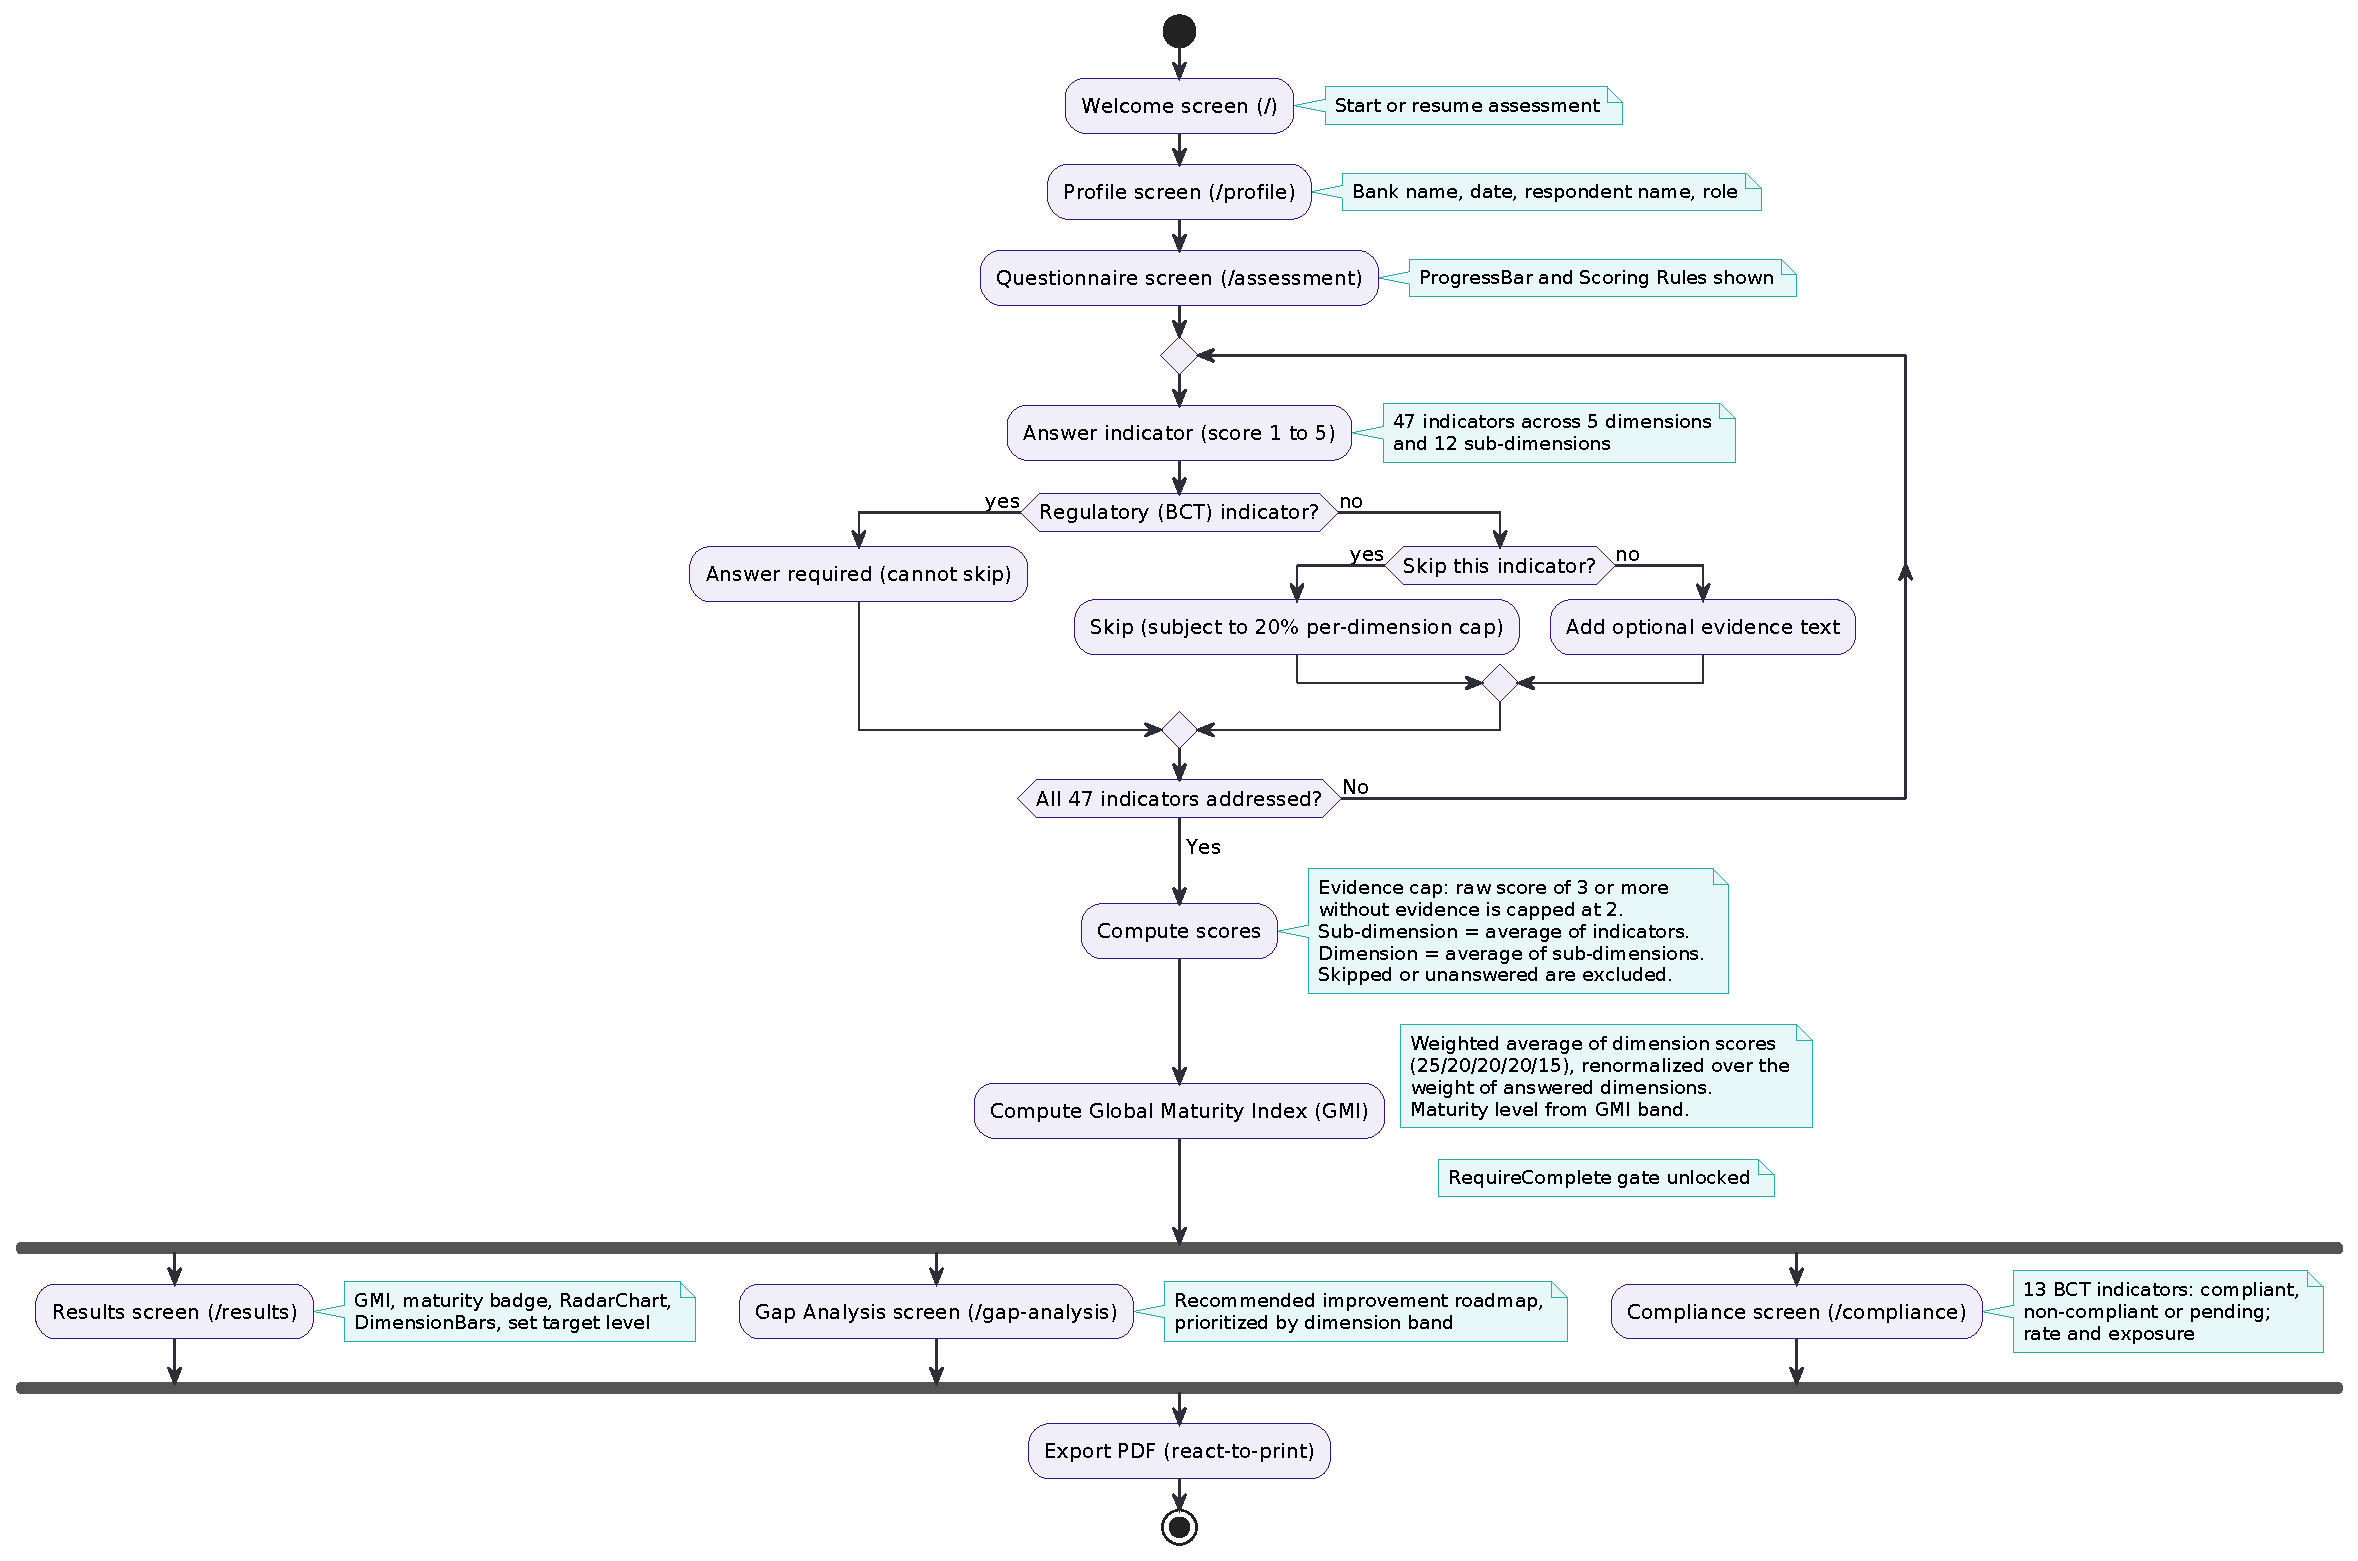
\includegraphics[width=0.95\textheight]{images/activity.pdf}
\caption{User flow and completion gate of DataPilot}
\label{fig:activity}
\end{sidewaysfigure}

\subsubsection{Solution Implementation}

The tool was implemented with the technologies described in Chapter 3. Its six screens realize the assessment workflow end to end, and each is shown as a live screenshot of the Iteration 3 build of the application in Figures~\ref{fig:screen-welcome} through~\ref{fig:screen-compliance} at the end of this subsection. In the Iteration 3 build, the Welcome screen introduces DataPilot as the data maturity steering tool and collects the session profile through an inline form, the bank name, the assessment date, the respondent name, and the role, whose start action stays disabled until all four fields are filled and then opens the Questionnaire directly. The Profile screen allows the same details to be reviewed or edited at any point during the session, and it also exposes a guarded reset that clears the stored assessment. The Questionnaire screen is the core data entry surface: it presents the 47 indicators grouped by dimension and sub-dimension, and for each indicator it displays the question, the guidance hint, the five level rubric as selectable options, an evidence field, and a skip control; it also shows the scoring rules and an overall progress indicator so the respondent always knows how much of the assessment remains. The skip control is disabled for the thirteen regulatory indicators and becomes unavailable once a dimension has reached its skip limit, and the evidence field is what determines whether a high score survives the evidence cap; a skipped indicator displays an undo control that restores it to the answerable state and frees the corresponding skip within the dimension ceiling, and a refused skip is explained by an explicit message naming the dimension and its ceiling. The Results dashboard presents the maturity profile through a Recharts radar chart that overlays the current score of each dimension on the selected target level, together with the Global Maturity Index (GMI) expressed both on the five point scale and as a percentage, the maturity level with its CMMI name and Gartner label, the computation formula displayed for auditability, and an interpretation grid stating the recommended action for each maturity level. The Gap Analysis screen ranks the twelve sub-dimensions by ascending score and assigns each sub-dimension one of four priority labels, critical below 2.0, high below 2.6, moderate below 3.4, and low at or above 3.4, and positions the five dimensions on an effort and impact matrix whose quadrants, quick wins, major projects, fill ins, and low priority, are derived from each dimension score and its weight. These four priority labels are the sizing signal, not the schedule: the labelled sub-dimensions are then grouped into three time-sequenced roadmap phases, a first phase of zero to three months dedicated to critical gaps and regulatory compliance, a second phase of three to six months dedicated to formalization and documentation, and a third phase of six to twelve months dedicated to optimization, each populated with the recommended actions of the dimensions it contains; any sub-dimension that carries a failing regulatory indicator or scores below 2.0 is forced into the first phase regardless of its label. The four priority labels therefore describe how far each sub-dimension is from target, while the three phases sequence the work over time. The Compliance screen reports a status per regulatory indicator, compliant when the effective score reaches three out of five, non compliant below that threshold, and pending when unanswered, together with the supporting evidence, the overall compliance rate computed as the share of the thirteen indicators that are compliant, and the resulting regulatory exposure level, which is rated low when the rate reaches eighty percent, medium when it reaches fifty percent, and high otherwise.

The computation behind the Compliance screen reuses the same scoring selectors as the Results dashboard rather than duplicating any logic. When the screen is opened, it requests the compliance summary from the store, which retrieves the thirteen regulatory indicators, evaluates the effective score of each through the evidence cap, classifies each as compliant, non compliant, or pending, and aggregates these classifications into the compliance rate and the exposure level before returning them for display. This sequence is shown in Figure~\ref{fig:sequence-compliance}, and it demonstrates that the regulatory view is a direct projection of the audited effective scores, so a bank cannot appear compliant on an indicator whose score was capped for lack of evidence.

\begin{figure}[H]
\centering
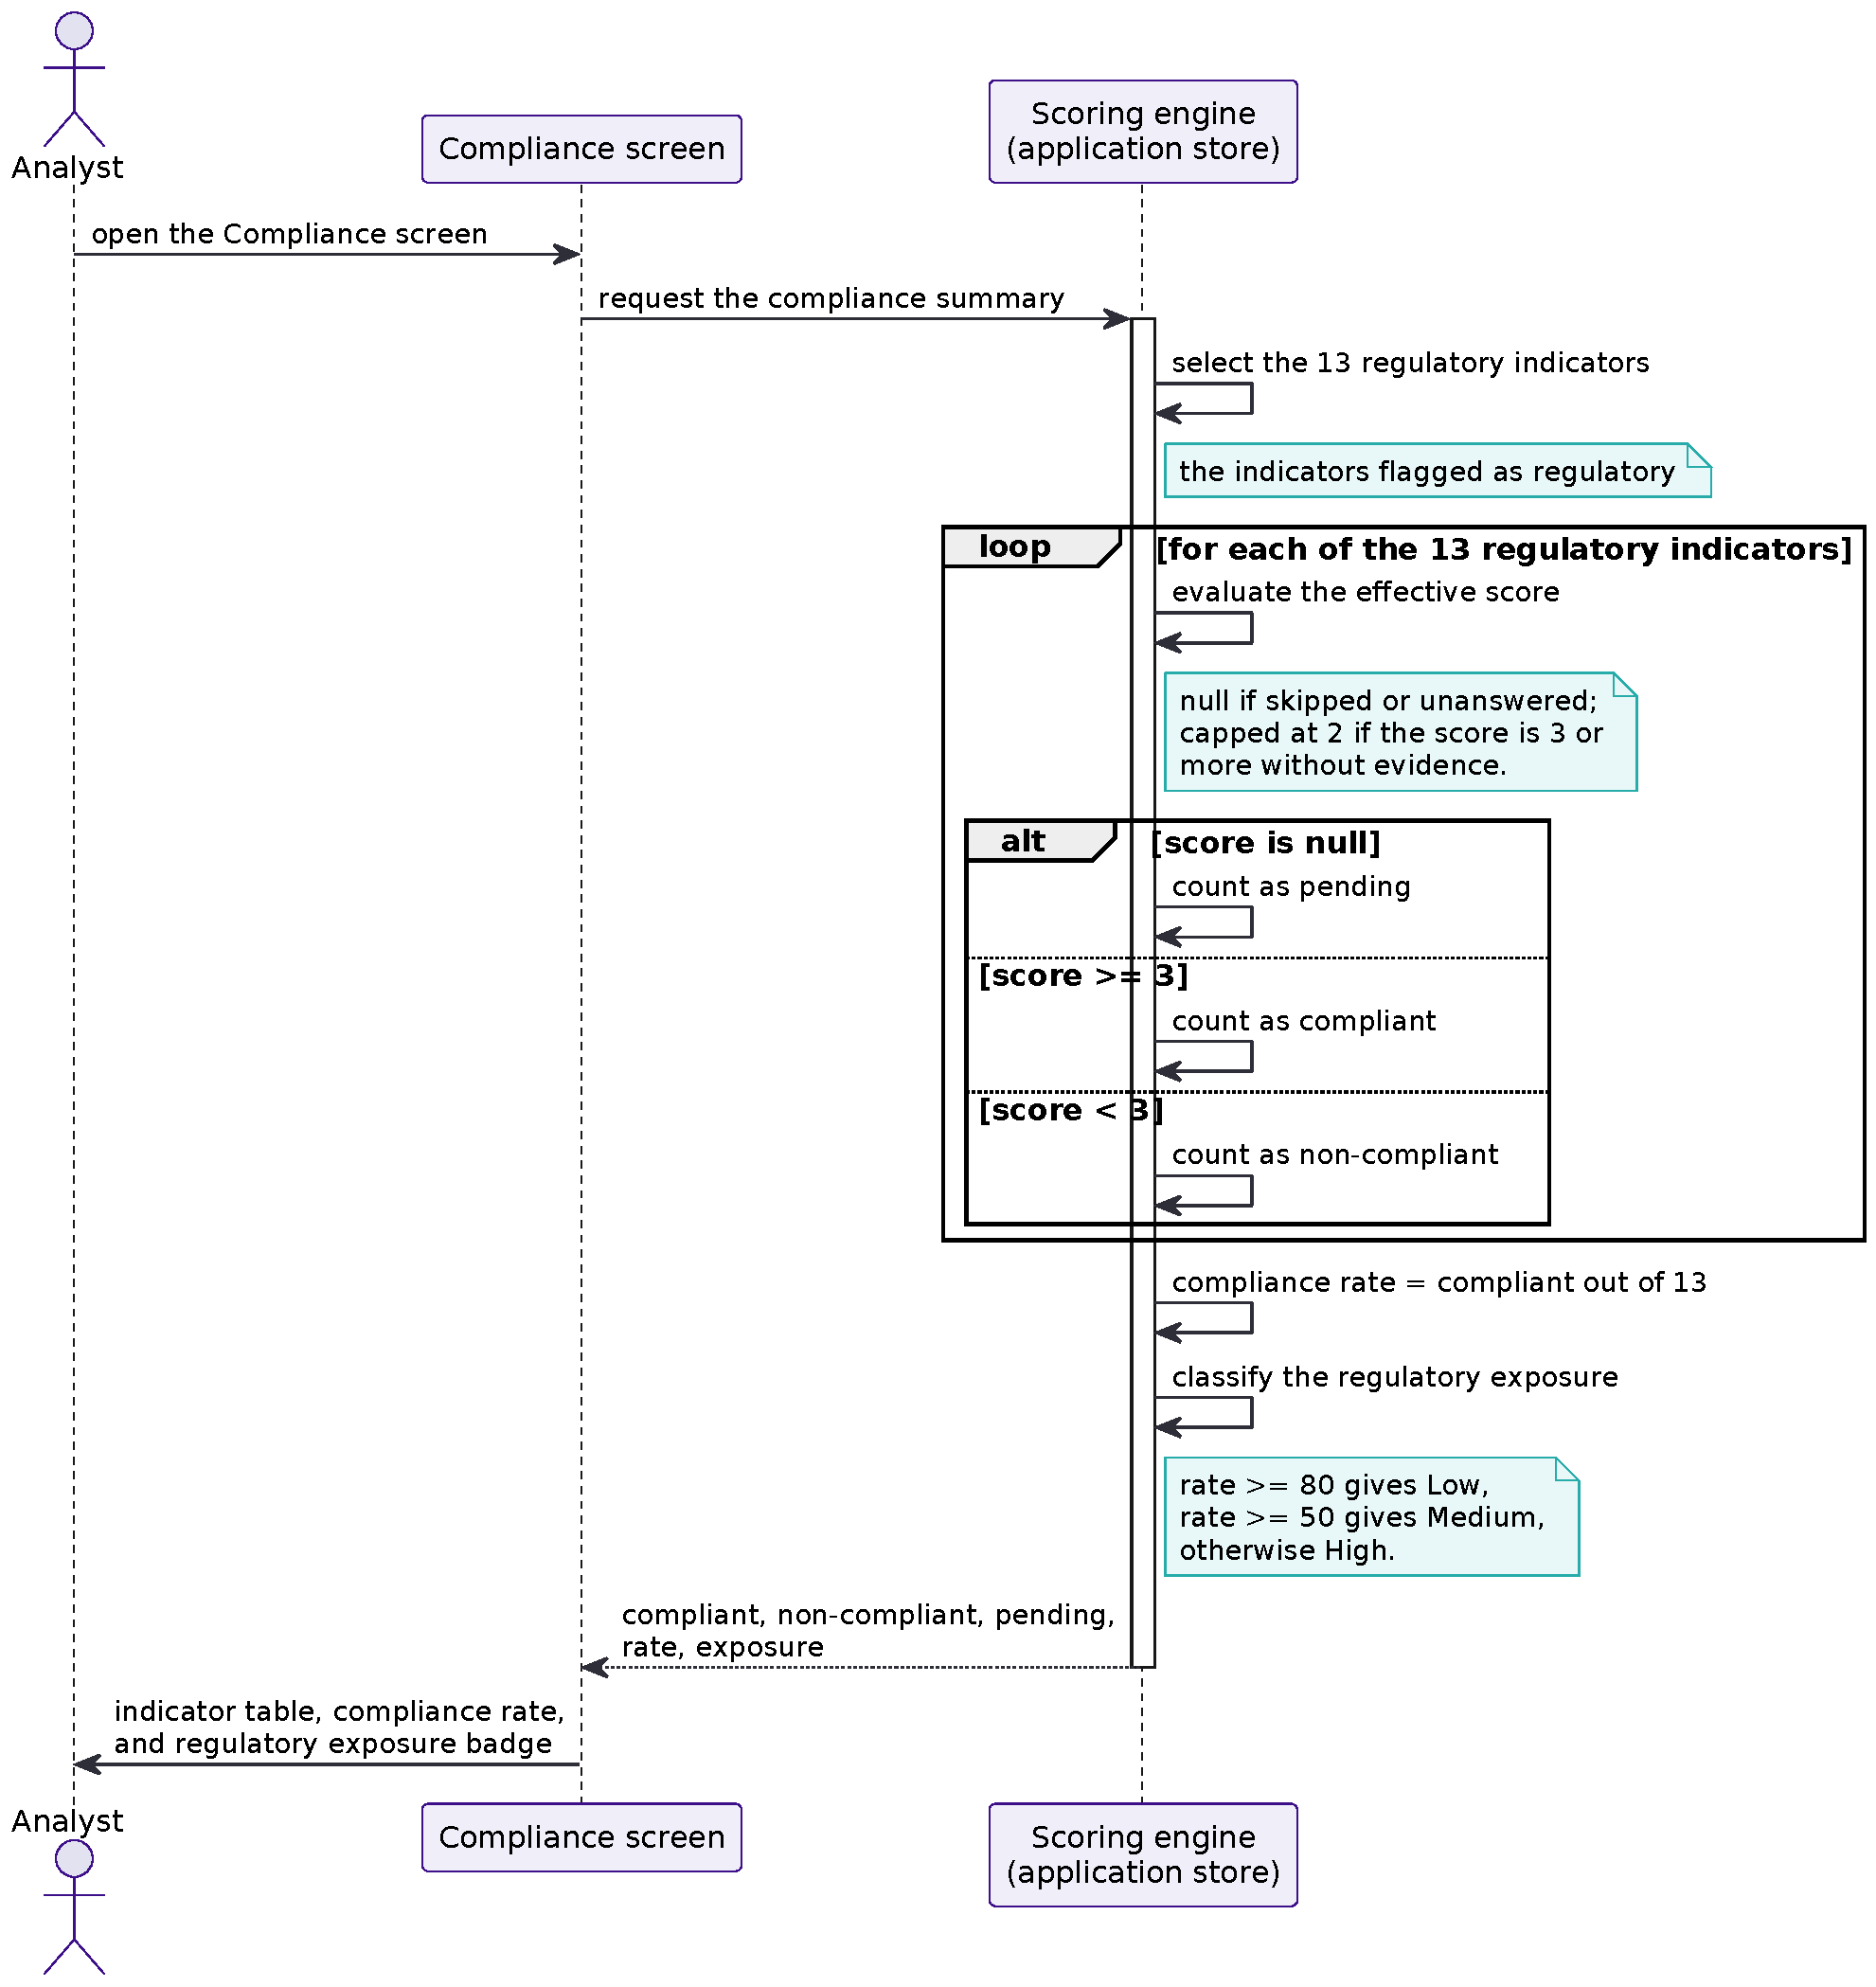
\includegraphics[width=0.9\textwidth]{images/sequence-compliance.pdf}
\caption{Sequence of the regulatory compliance computation}
\label{fig:sequence-compliance}
\end{figure}

The six screens of the Iteration 3 build are shown below. Figure~\ref{fig:screen-welcome} shows the Welcome screen and Figure~\ref{fig:screen-profile} the Profile form. Figure~\ref{fig:screen-questionnaire} shows the Questionnaire, the core data entry surface. Figures~\ref{fig:screen-results}, \ref{fig:screen-gap}, and \ref{fig:screen-compliance} show the Results dashboard, the Gap Analysis screen, and the BCT Compliance screen for a representative assessment. The Results, Gap Analysis, and Compliance captures were produced from a complete demonstration session of the 47 indicators, which is why the completion gate allows them to render.

\begin{figure}[H]
\centering
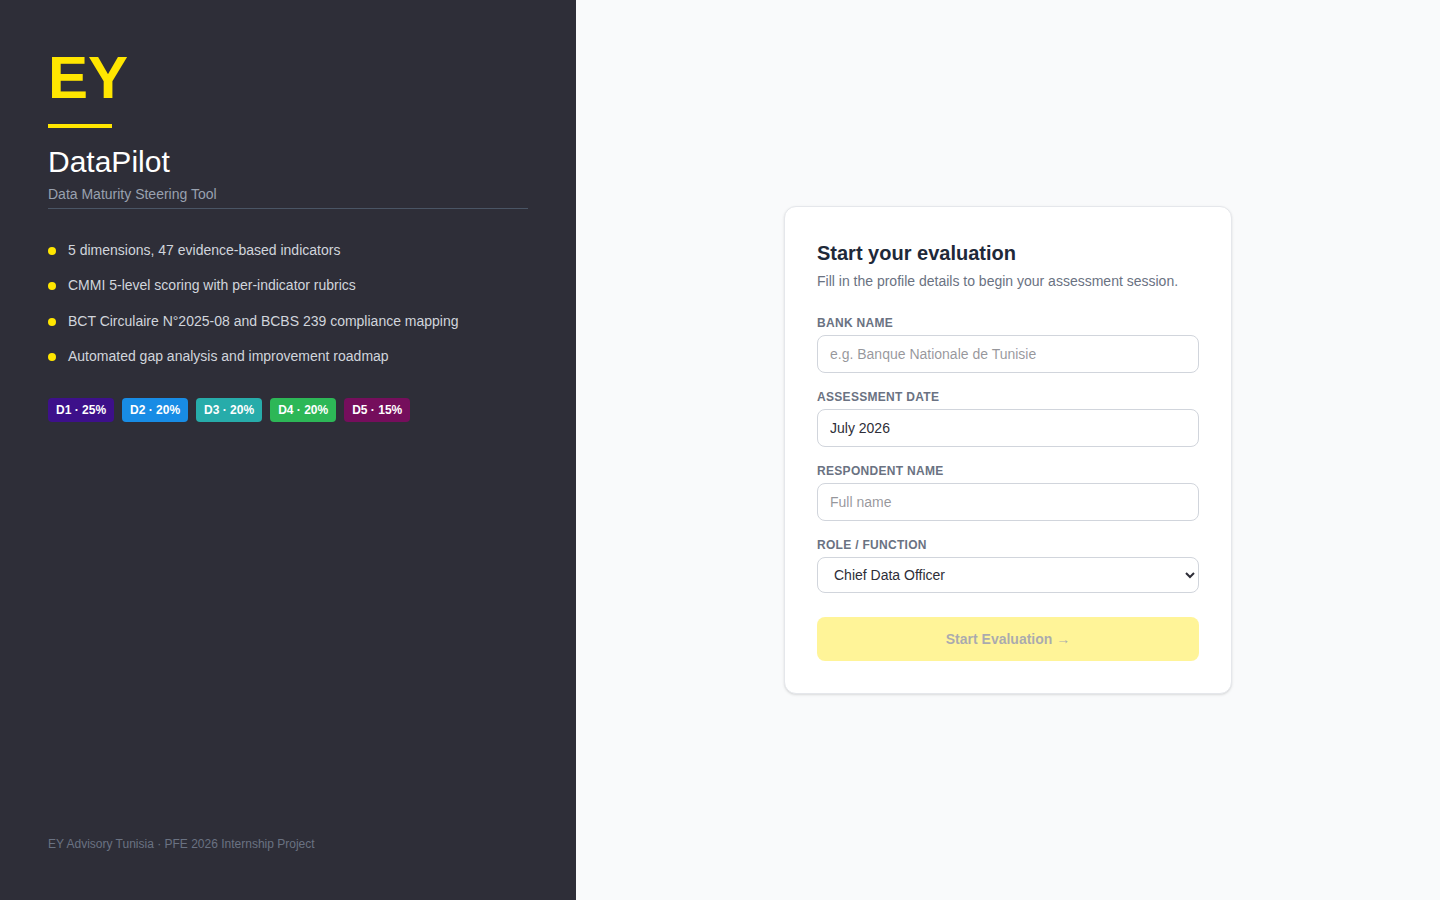
\includegraphics[width=0.85\textwidth]{images/screen-welcome.png}
\caption{DataPilot Welcome screen}
\label{fig:screen-welcome}
\end{figure}

\begin{figure}[H]
\centering
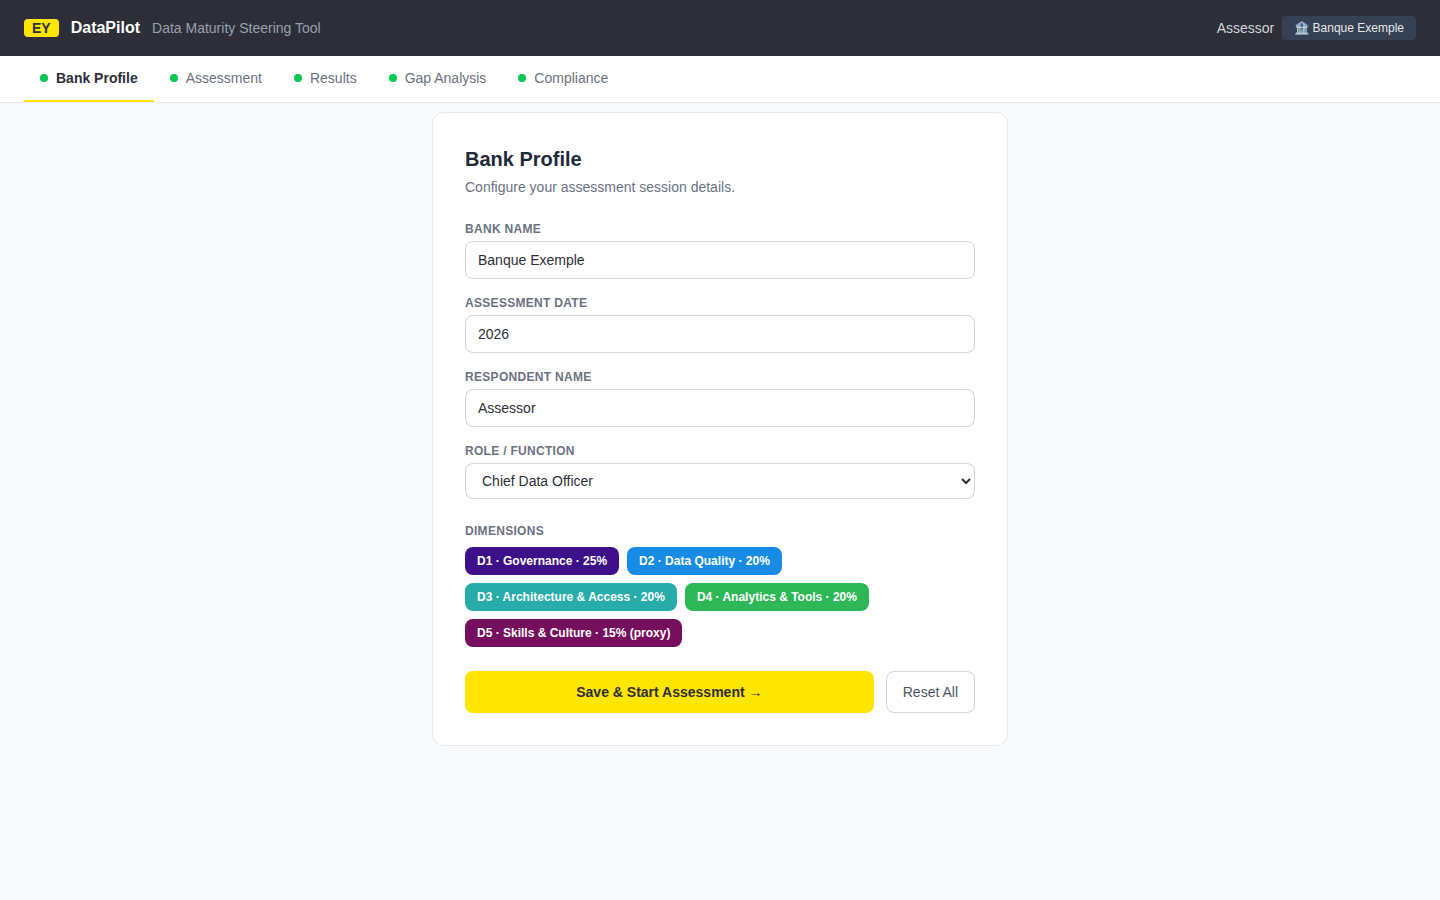
\includegraphics[width=0.85\textwidth]{images/screen-profile.png}
\caption{DataPilot Profile screen}
\label{fig:screen-profile}
\end{figure}

\begin{figure}[H]
\centering
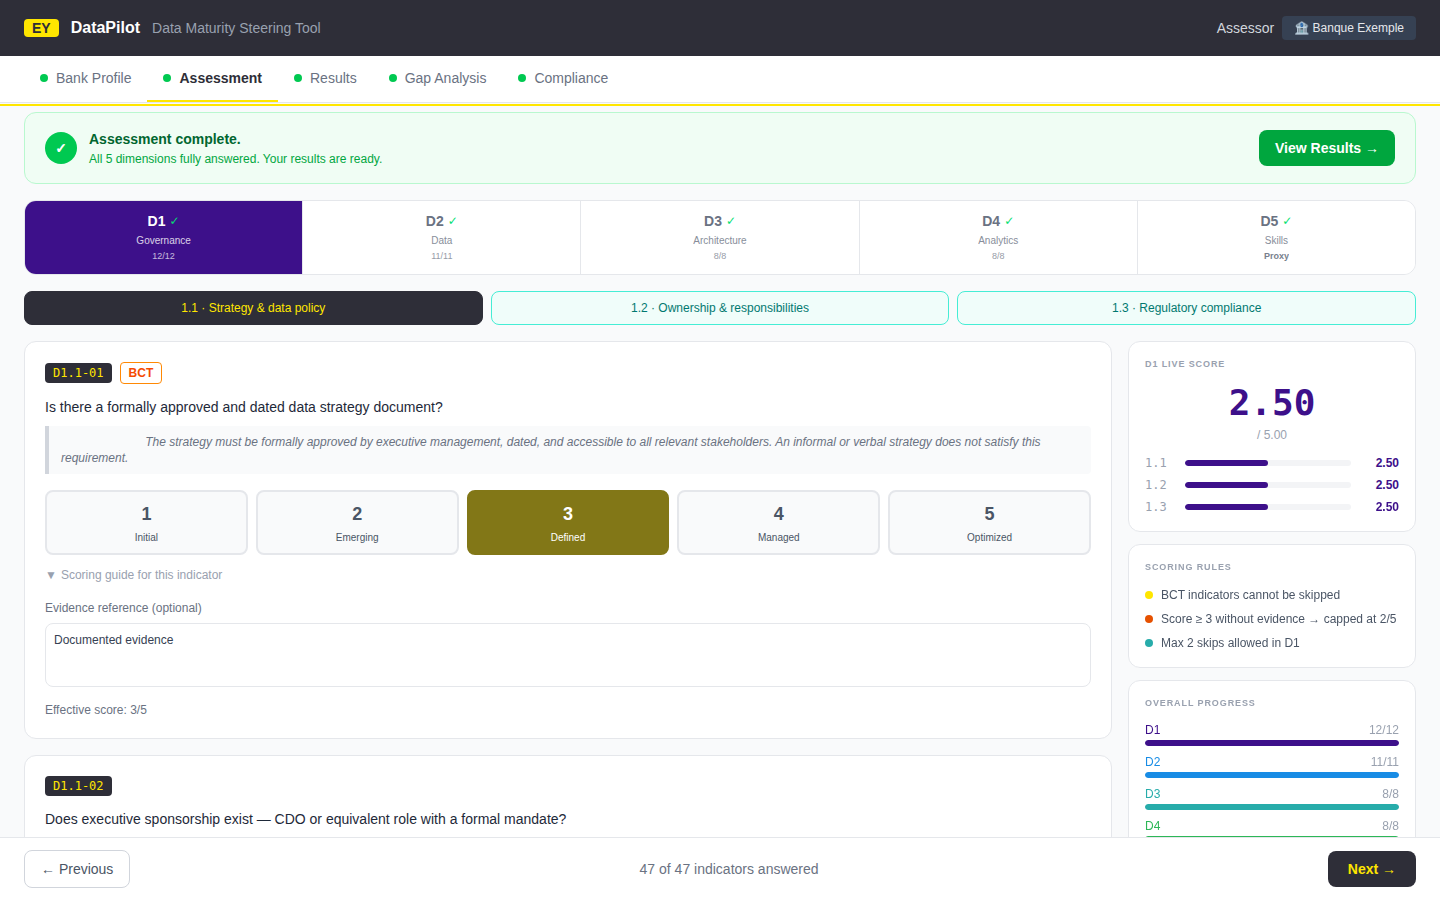
\includegraphics[width=0.92\textwidth]{images/screen-questionnaire.png}
\caption{DataPilot Questionnaire screen}
\label{fig:screen-questionnaire}
\end{figure}

\begin{figure}[H]
\centering
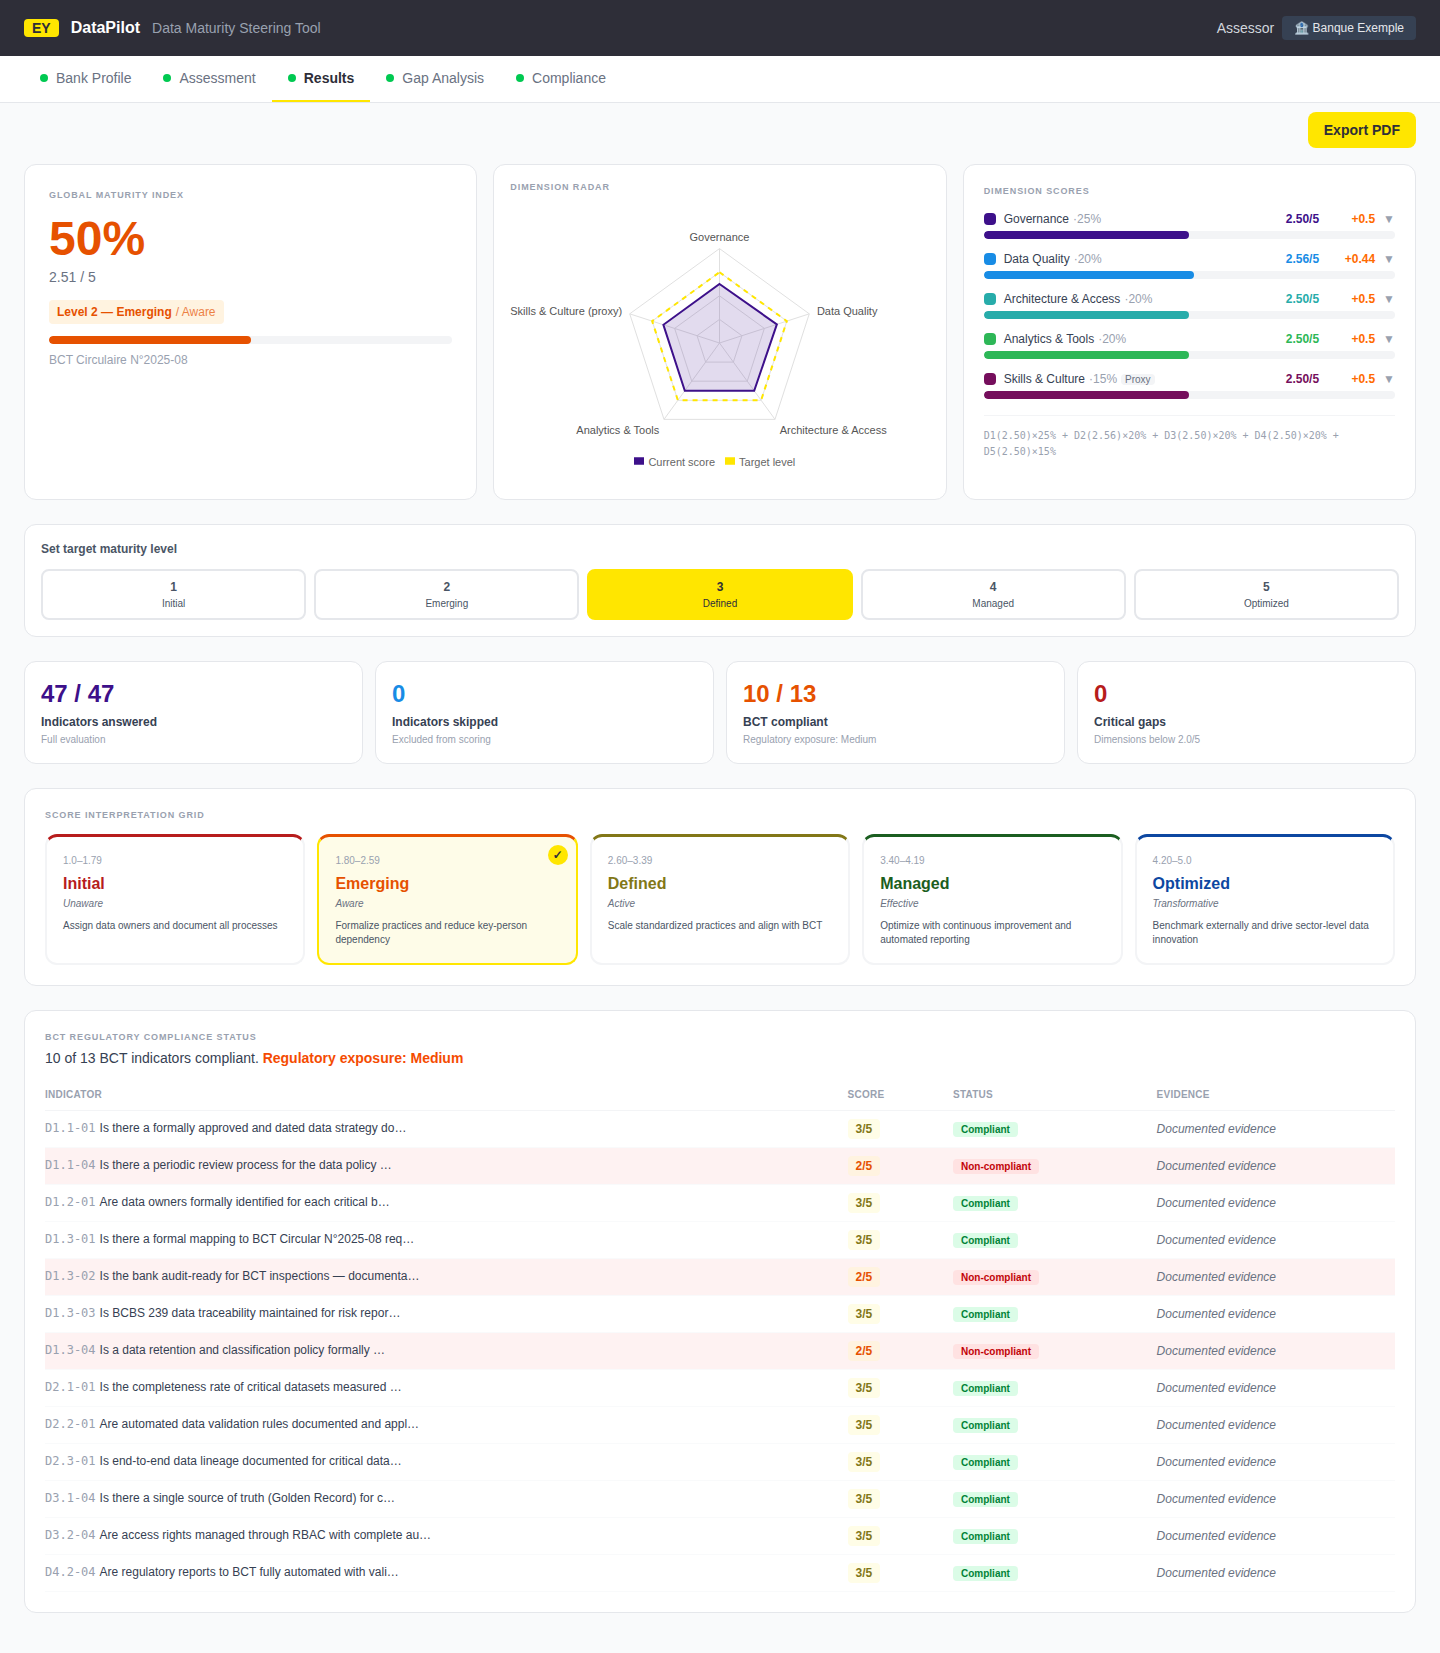
\includegraphics[width=0.92\textwidth]{images/screen-results.png}
\caption{DataPilot Results dashboard}
\label{fig:screen-results}
\end{figure}

\begin{figure}[H]
\centering
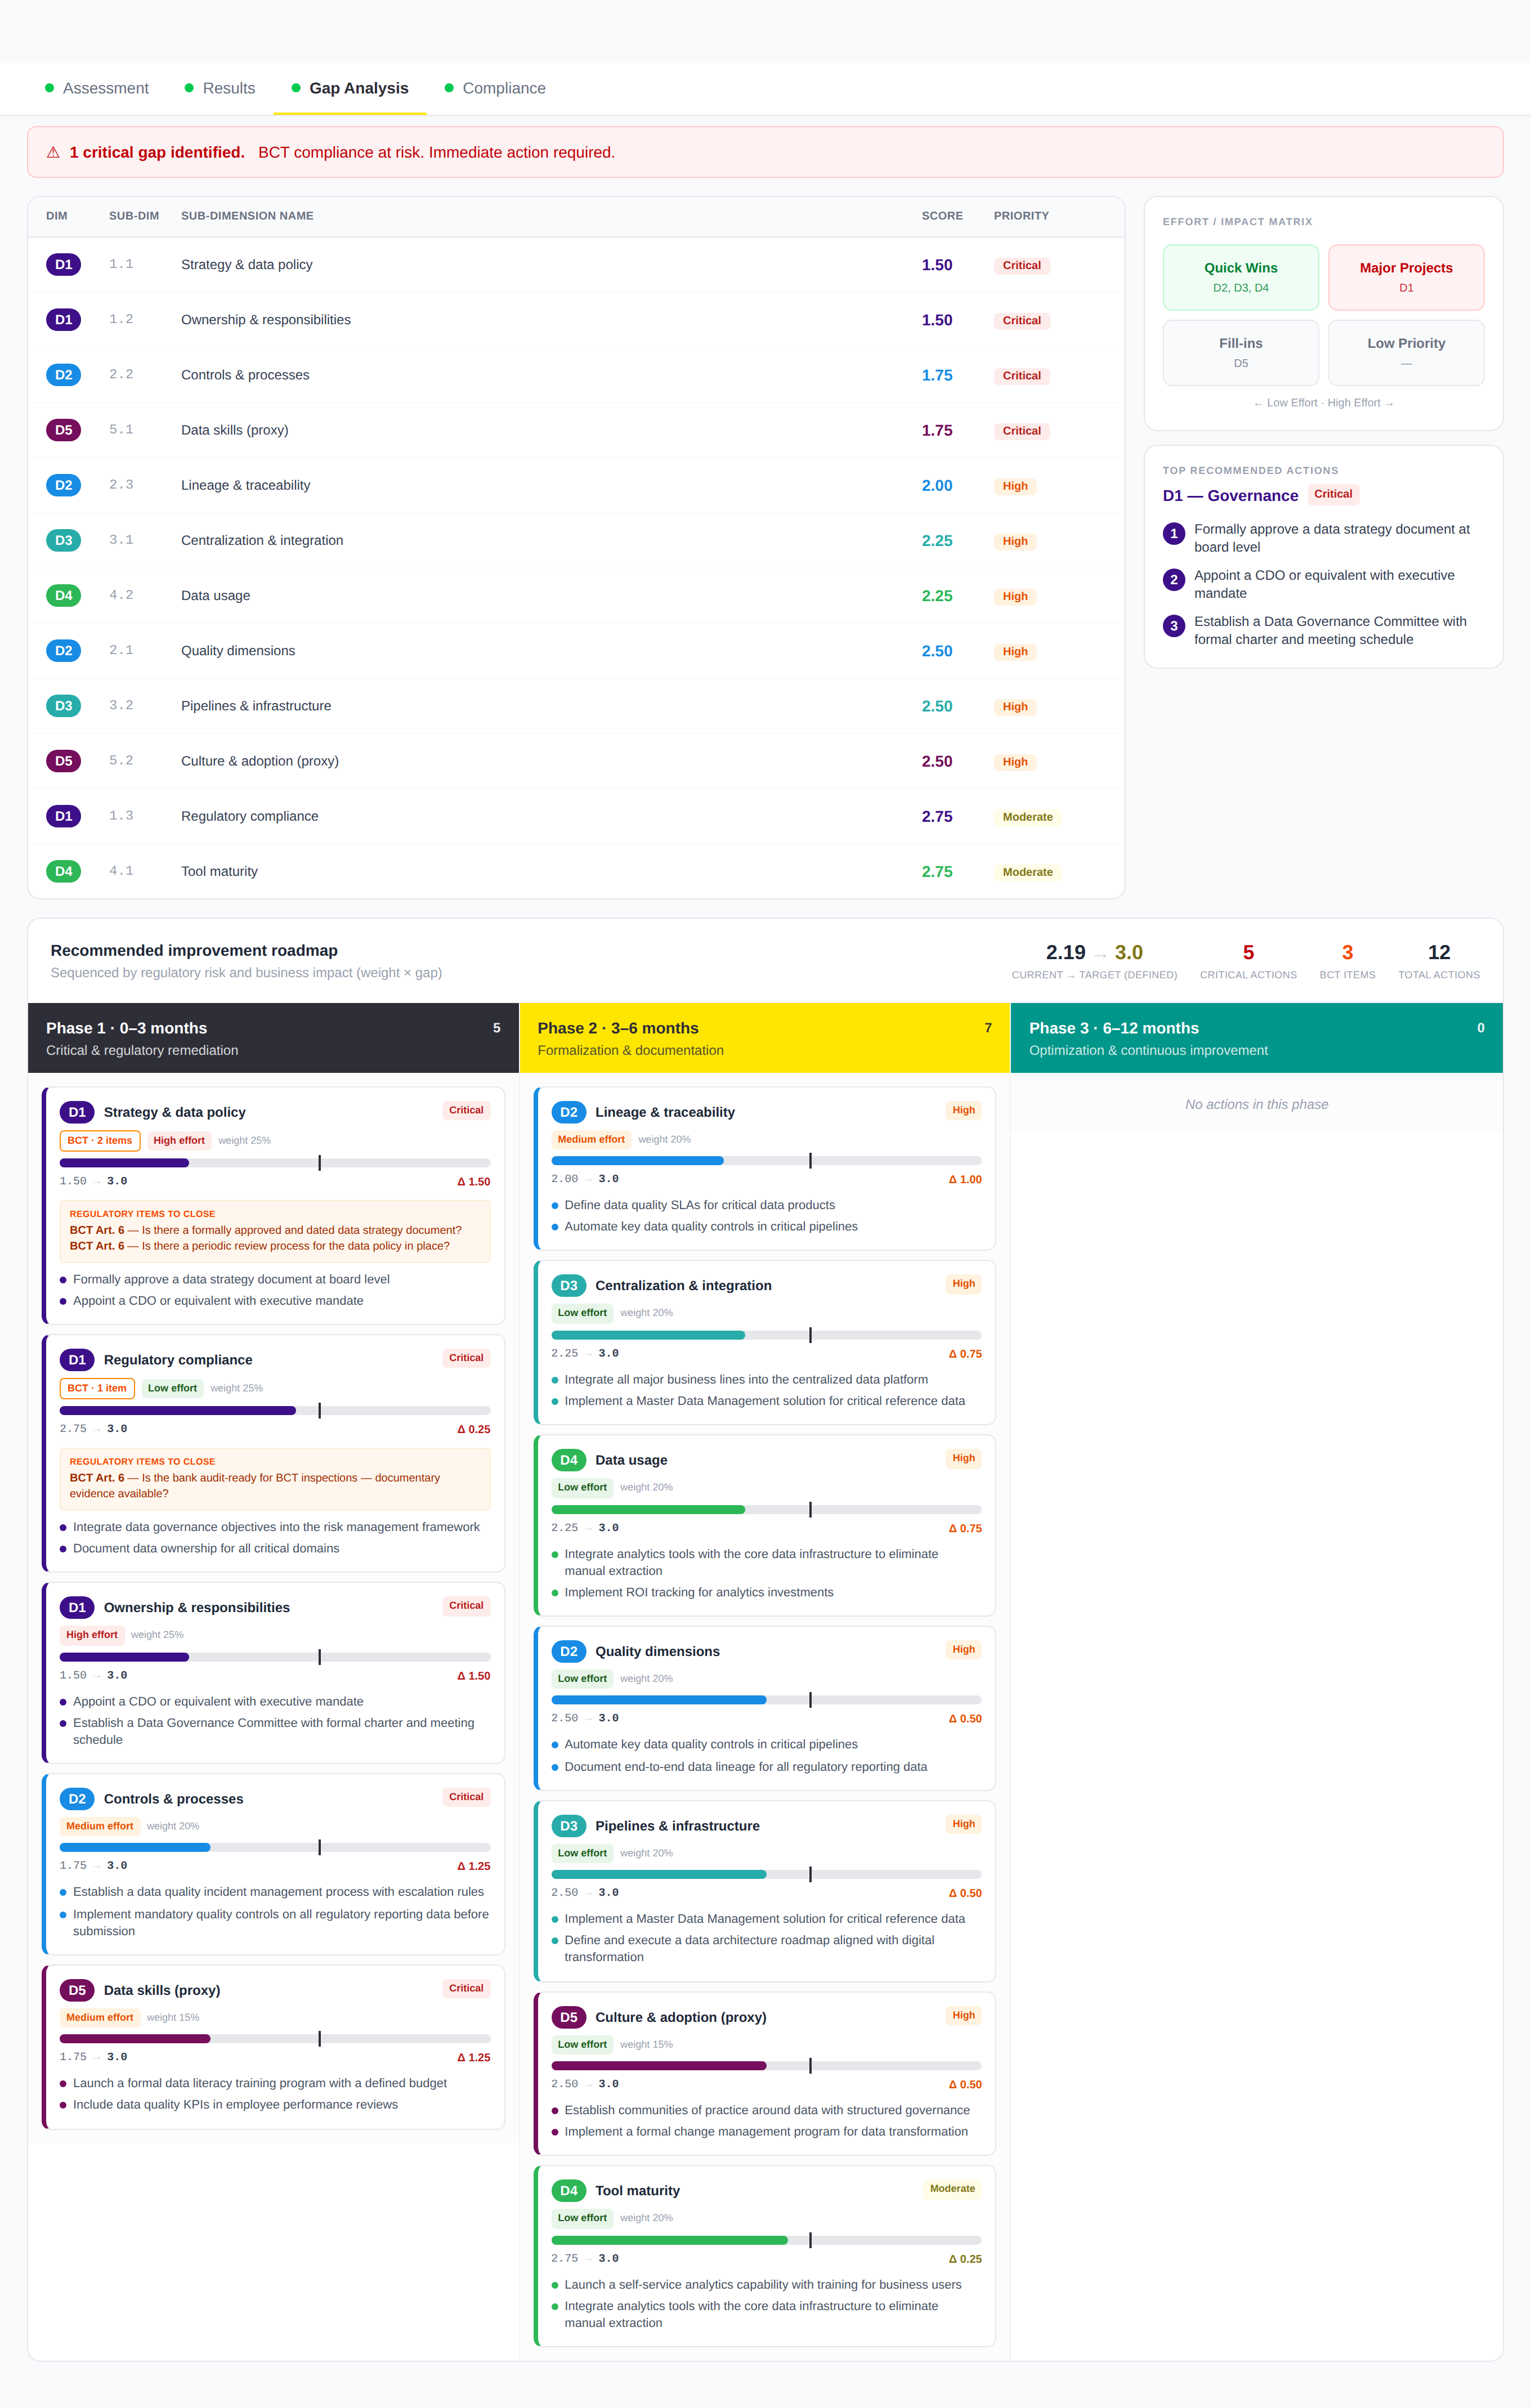
\includegraphics[width=0.78\textwidth]{images/screen-gap.png}
\caption{DataPilot Gap Analysis screen}
\label{fig:screen-gap}
\end{figure}

\begin{figure}[H]
\centering
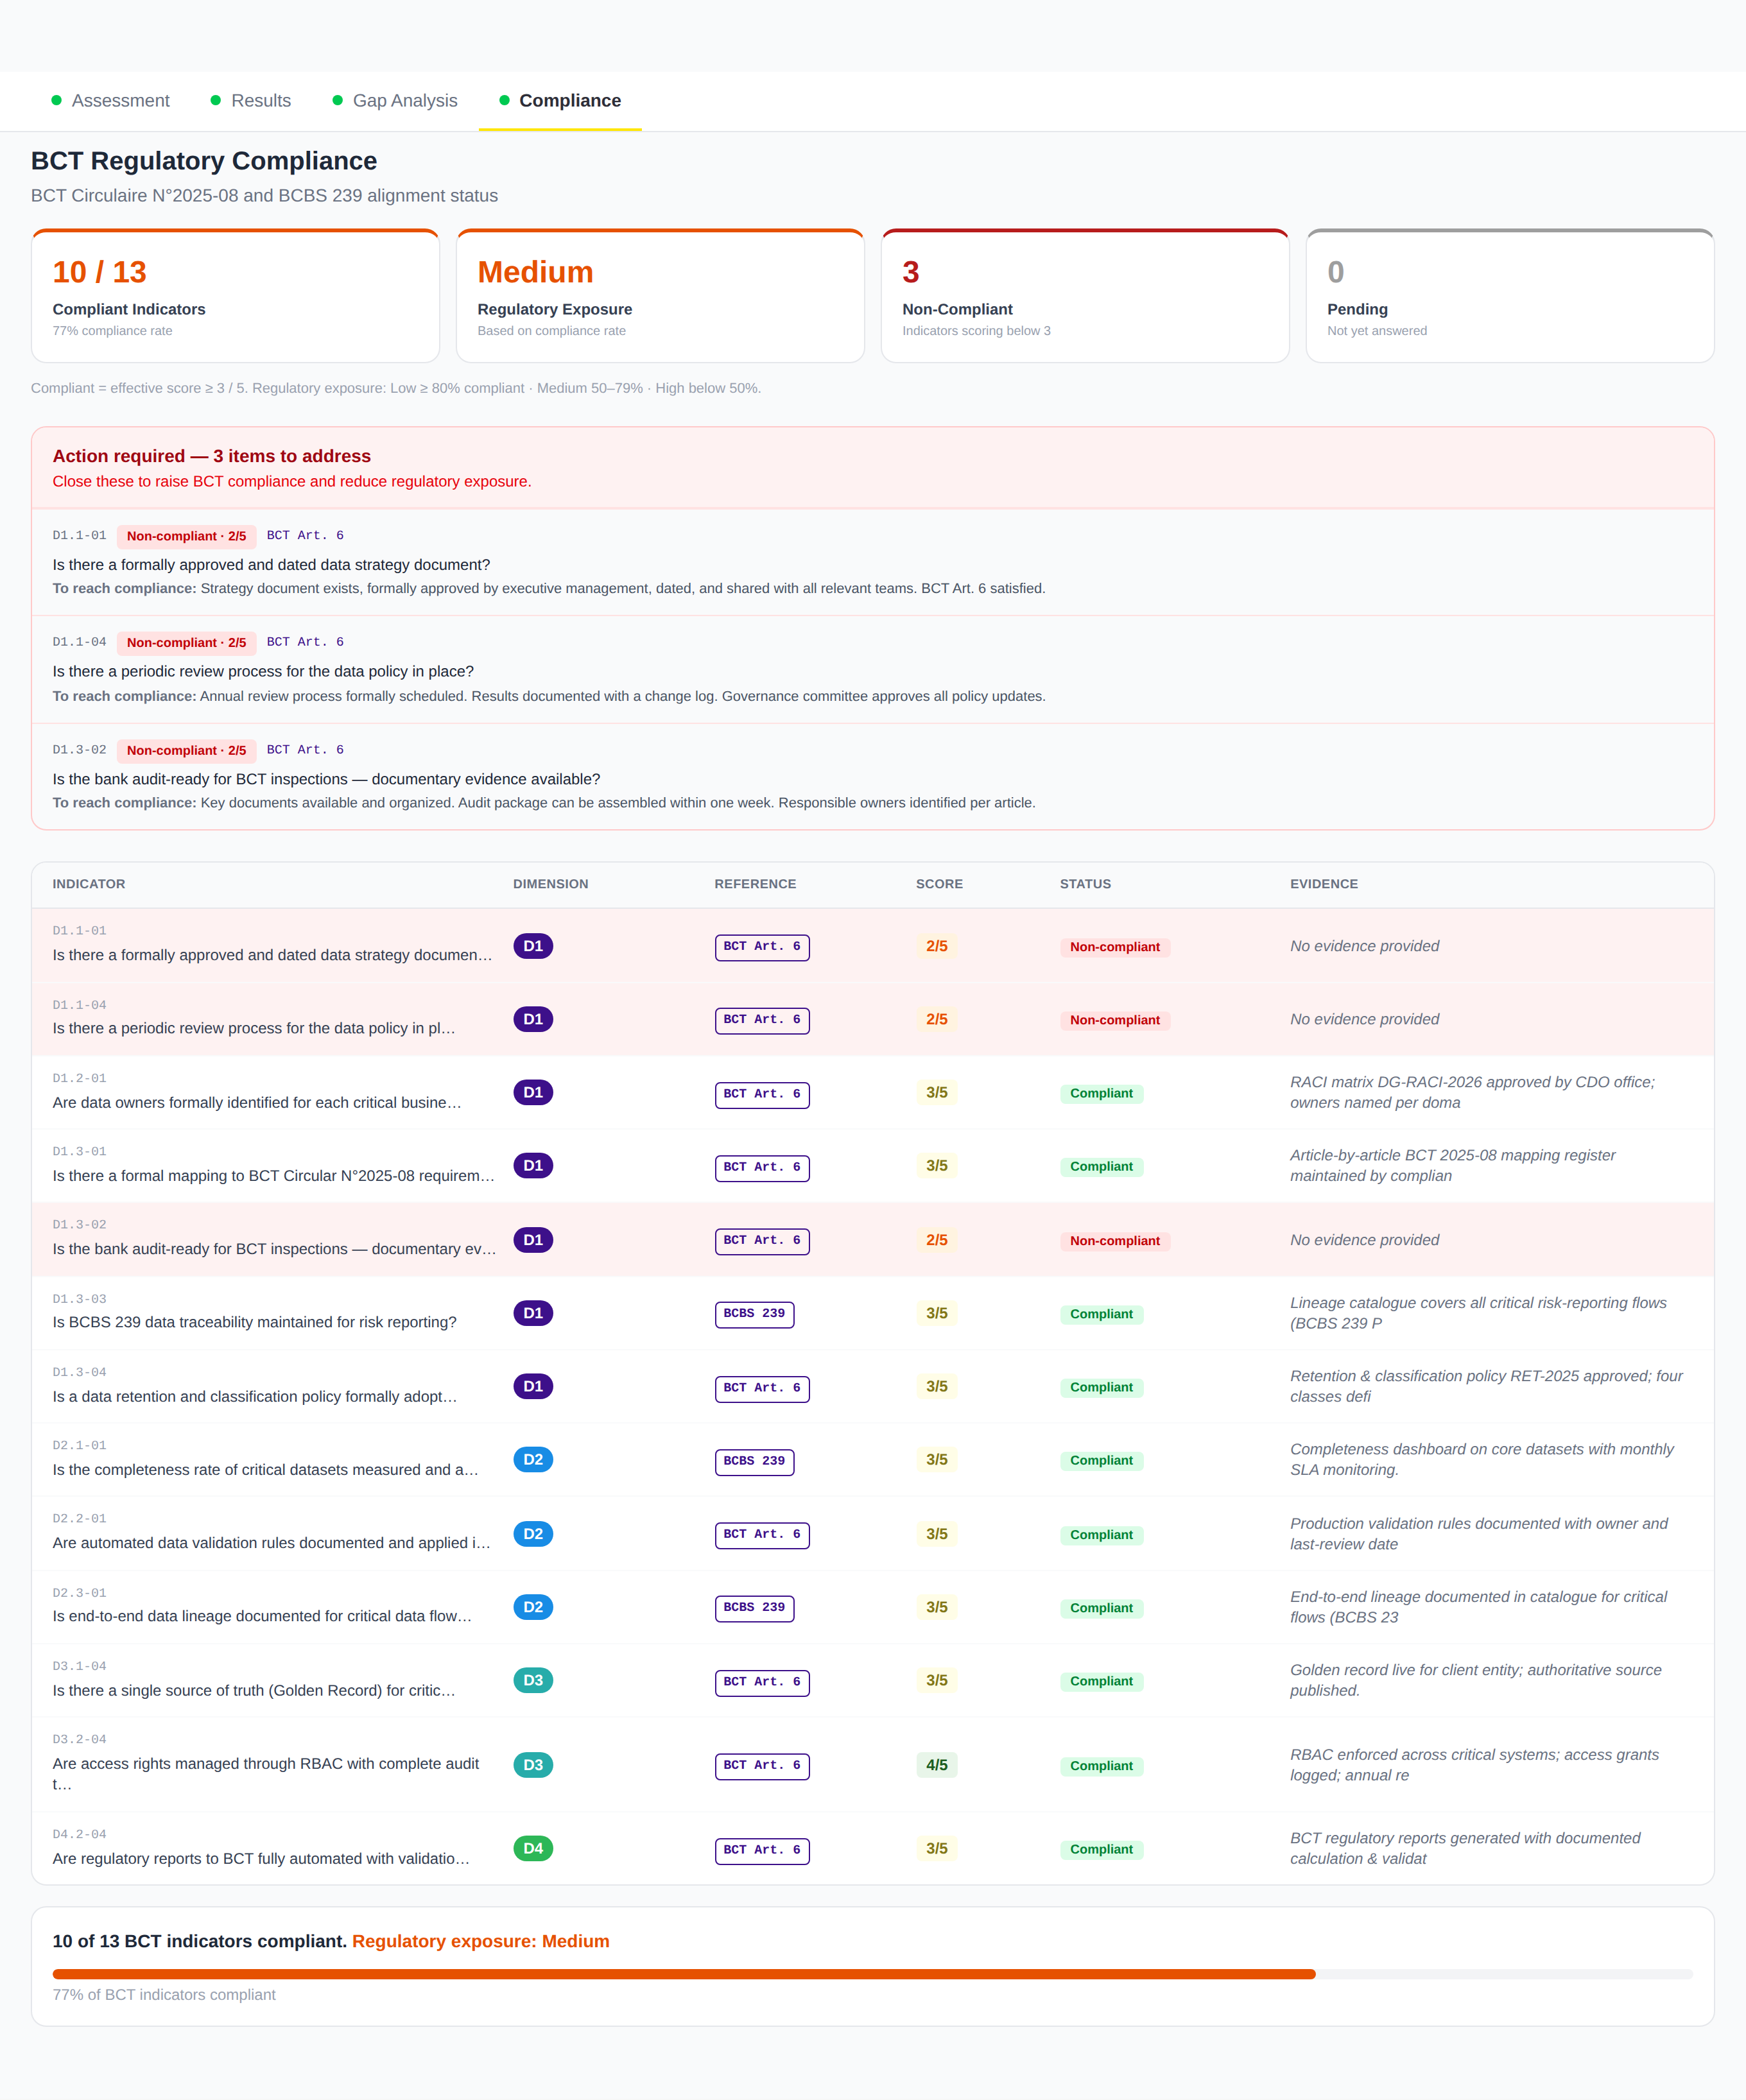
\includegraphics[width=0.9\textwidth]{images/screen-compliance.png}
\caption{DataPilot Compliance screen}
\label{fig:screen-compliance}
\end{figure}

\subsubsection{Solution Evaluation}

The tool was evaluated through functional testing on simulated banking data: complete assessment scenarios were entered by hand and each business rule was exercised at its boundary, screen by screen, so that the evaluation evidence consists of named, reproducible behaviors rather than a general assertion of correctness. Five scenarios carry the core of this evidence. First, the evidence cap: an indicator claimed at four out of five with the evidence field left empty was computed as an effective two and flagged as capped, visibly reducing its sub-dimension and dimension scores, which is exactly the anti-inflation behavior specified in Iteration 2. Second, the regulatory lock: the skip control remained disabled on each of the thirteen regulatory indicators, and a skip request on a regulatory indicator was refused, so the regulatory core of the questionnaire cannot be evaded. Third, the skip ceiling: after two indicators of Governance had been skipped, a third skip request within that dimension was refused, its ceiling being two, and the corresponding control became unavailable. Fourth, the completion gate: opening the Results route while a dimension remained unanswered redirected back to the Questionnaire, and the dashboards rendered only once all five dimensions were complete. Fifth, the compliance projection: a regulatory indicator whose effective score fell below three surfaced on the Compliance screen as non compliant, and the displayed compliance rate and exposure level matched a manual count over the thirteen regulatory indicators.

Beyond the rule boundaries, a representative complete session of all 47 indicators reproduced the illustrative profile detailed in the results of Chapter 5, a Global Maturity Index of 2.19 out of 5, displayed as 44\% and as Level 2, Emerging, and recomputing the weighted sum by hand from the per-dimension scores confirmed that the displayed index matches the methodology of Iteration 2 exactly. The captured demonstration session shown in Figures~\ref{fig:screen-results} through~\ref{fig:screen-compliance} is a second complete session, also within the emerging band, whose displayed index and compliance summary were retraced in the same way, and closing and reopening the browser restored the same session from the local storage, confirming persistence. Because this validation is scenario based rather than automated, it confirms the exercised paths but cannot rule out untested edge cases; the absence of an automated test suite is recorded as a limitation and taken up in the future work. Within that boundary, the evaluation confirmed that the tool reproduces the scoring methodology faithfully and presents the results in an actionable form, which addresses research question RQ3; the consolidated results the instrument produces are presented in Chapter 5. The evaluation also delimited the artifact: one assessor, one browser, one bank, with the assessment record held only in that browser. Turning the validated instrument into a platform that a whole bank can operate under EY administration is the problem the fourth and final iteration addresses.

\subsection{Iteration 4: The Multi-Tenant Platform and Role Model}

In plain terms, Iteration 4 turns the single-user tool into a shared platform for many banks at once. Each bank works in its own isolated space that no other bank can see, EY administers a shared master questionnaire that each bank copies, and once a bank finalizes its assessment that record can no longer be quietly changed. The mechanics below implement exactly these guarantees.

The fourth iteration scales the single-user tool into a multi-tenant platform with a role model, so that a whole institution can contribute to one assessment under EY oversight. It follows the five activities of the regulative cycle a final time.

\subsubsection{Problem Investigation}

The evaluation of Iteration 3 validated the instrument and, in the same movement, delimited it: one assessor, one browser, one bank, with the assessment record held only in that browser. The fourth iteration consumes those evaluation findings as its problem investigation, which is the DSR bridge between the two iterations: what the previous evaluation recorded as boundaries of the artifact becomes the problem statement of its successor. Three problem strands were identified.

First, one bank is not one assessor. A real maturity assessment draws on several functions of the institution: the governance and compliance function is best placed to answer the Governance dimension, the quality function answers Data Quality, the information technology department answers Architecture and Access, and so on. The Iteration 3 artifact confines the whole questionnaire to a single browser profile: contributors cannot divide the work along their responsibilities, and a coordinator cannot watch progress or consolidate a single institutional result.

Second, EY needs oversight across engagements. DataPilot is an EY Advisory instrument: EY must be able to maintain the reference questionnaire centrally, onboard each client bank onto the tool, and review the submissions of every engagement. None of this is possible with a client-side artifact whose data never leaves an assessor's machine.

Third, confidentiality must be redefined across tenants. Once several banks share one platform, the confidentiality argument of Iteration 3, namely that the data never leaves the machine, no longer applies. It must be replaced by strict per-bank isolation: no bank may ever read another bank's answers, submissions, users, or tailored questionnaire.

A secondary problem completes the investigation: banks may need to tailor question wording or emphasis to their organization, while EY must keep one canonical reference instrument. The framework content must therefore become governed data rather than code, without the scoring rules becoming negotiable.

The success criteria of the iteration follow directly from these strands: role-scoped capabilities enforced on the server side, tenant isolation enforced at the data layer, a collaborative assessment that still produces one auditable submission per bank, and the preservation of every scoring rule of Iteration 2.

\subsubsection{Solution Design}

The platform was designed around five decisions.

\begin{sloppypar}
The first decision is a four-role hierarchy with numeric ranks. The EY Admin (owner), rank 3, has scope over all banks: it maintains the EY master template of the questionnaire, reviews submissions across banks, and invites each bank's Super Admin. The Super Admin, rank 2, is scoped to one bank: it manages the bank's departments, invites Admins, and manages roles and accounts within the bank. The Admin, rank 1, is likewise scoped to one bank: it edits the bank copy of the questionnaire, runs the group assessment, and invites Analysts. The Analyst, rank 0, is scoped to itself: it fills and submits assessments. Capabilities strictly decrease with rank, and the rank order is declared once, as \texttt{ROLE\_RANK = \{ analyst: 0, admin: 1, superadmin: 2, owner: 3 \}} in the server module \texttt{api/\_roles.js}, mirrored in \texttt{src/lib/roles.js} on the client. An unknown or corrupt role receives rank minus one and therefore fails every gate, so the role model fails closed by construction. The EY Admin deliberately has no bank of its own, and the bank name is the tenant key attached to every scoped row; there is no separate banks table, a deliberate design choice that keeps the tenancy model to a single column carried by every scoped record. The hierarchy and its scopes are shown in Figure~\ref{fig:role-hierarchy}, and a complete matrix of which role may perform each platform capability is given in Appendix~C. It is worth being precise about how bank management fits this model, since the dashboards are opened by the Analyst who runs the assessment rather than by an executive. Management consumes the assessment through its outputs rather than by operating the tool: the analyst produces the results, the coordinator finalizes them into one auditable submission, and the printable export carries the maturity profile, the gap analysis, and the compliance status to management and, through the EY Admin's cross-bank review, to the engagement. A dedicated read-only role for an executive who prefers to browse the live dashboards rather than receive the export is a natural extension identified for future work.
\end{sloppypar}

\begin{figure}[H]
\centering
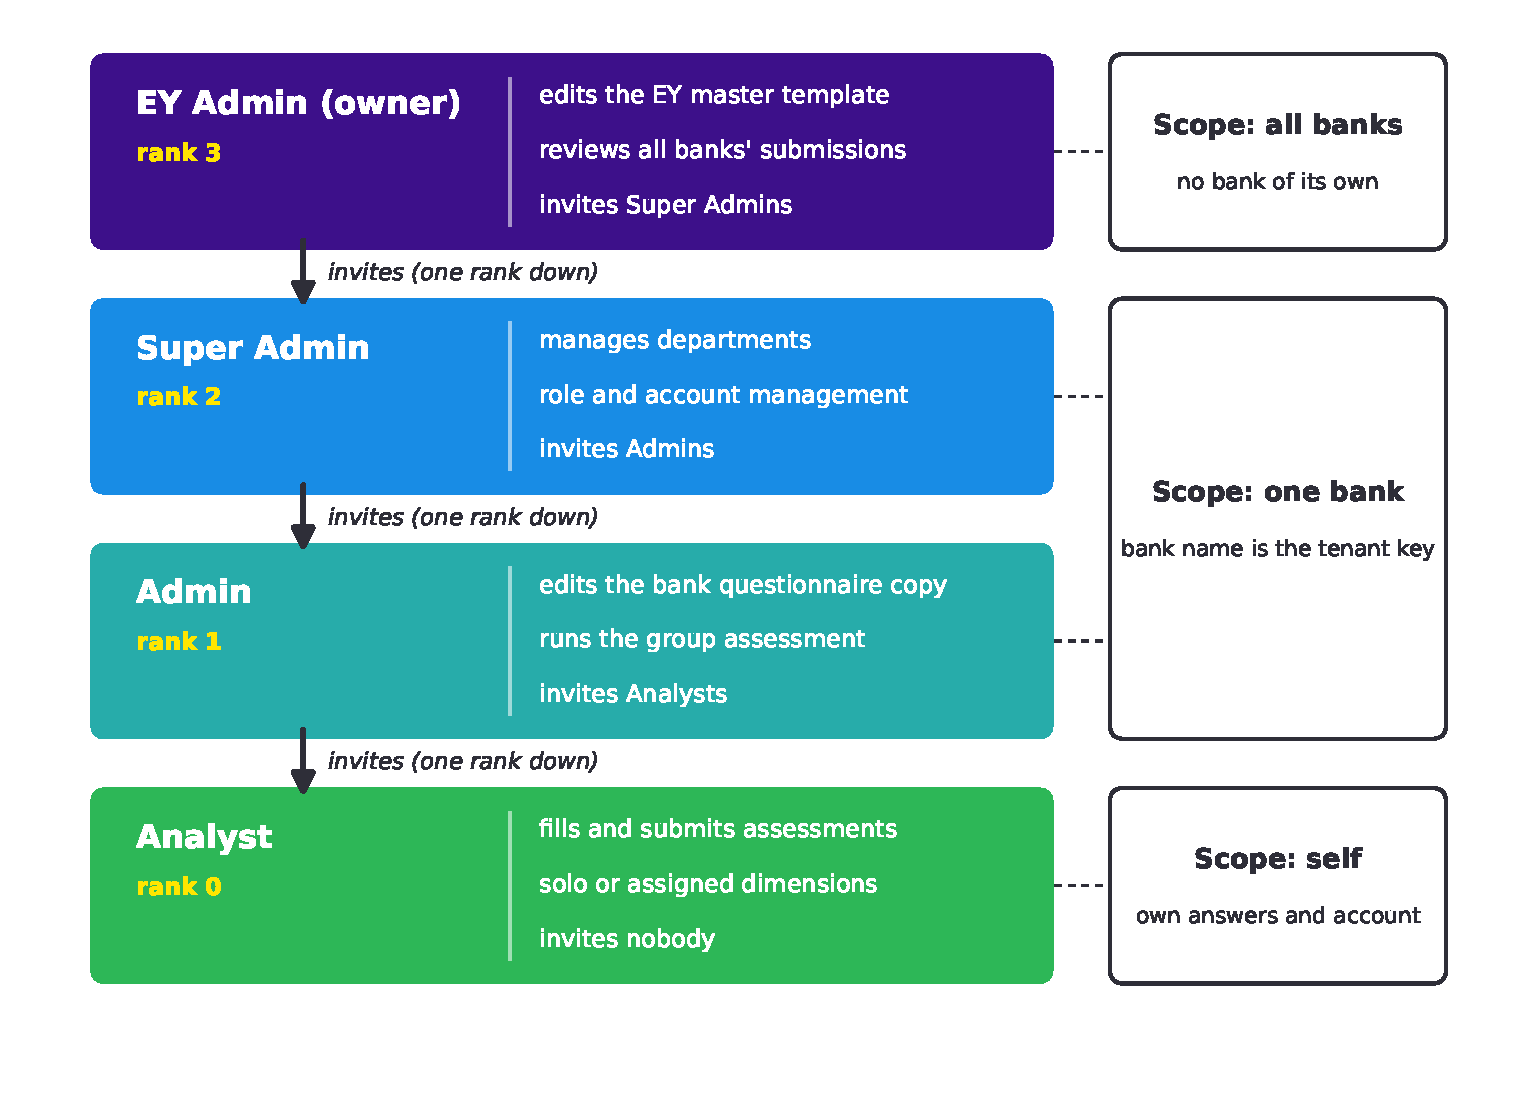
\includegraphics[width=0.8\textwidth]{images/role-hierarchy.pdf}
\caption{The four-role hierarchy and its scopes}
\label{fig:role-hierarchy}
\end{figure}

\begin{sloppypar}
The second decision is a top-down, invite-only onboarding chain. Public sign-up is disabled entirely, and the login screen offers no account creation. Each role can invite exactly one rank below itself, a rule computed on the server as \texttt{invitableRole(callerRole)}: the EY Admin invites a bank's Super Admin and names the bank, which creates the tenant; the Super Admin invites Admins; the Admin invites Analysts. Everyone below the EY Admin inherits the inviter's bank, and the invited person never types their own identity: the inviter sets the email, the function, the bank, and optionally the department, and the invitee only sets a password from the invitation email link. The \texttt{invited\_by} lineage recorded on every profile yields each bank's organization tree. The onboarding sequence is shown in Figure~\ref{fig:sequence-onboarding}.
\end{sloppypar}

\begin{figure}[H]
\centering
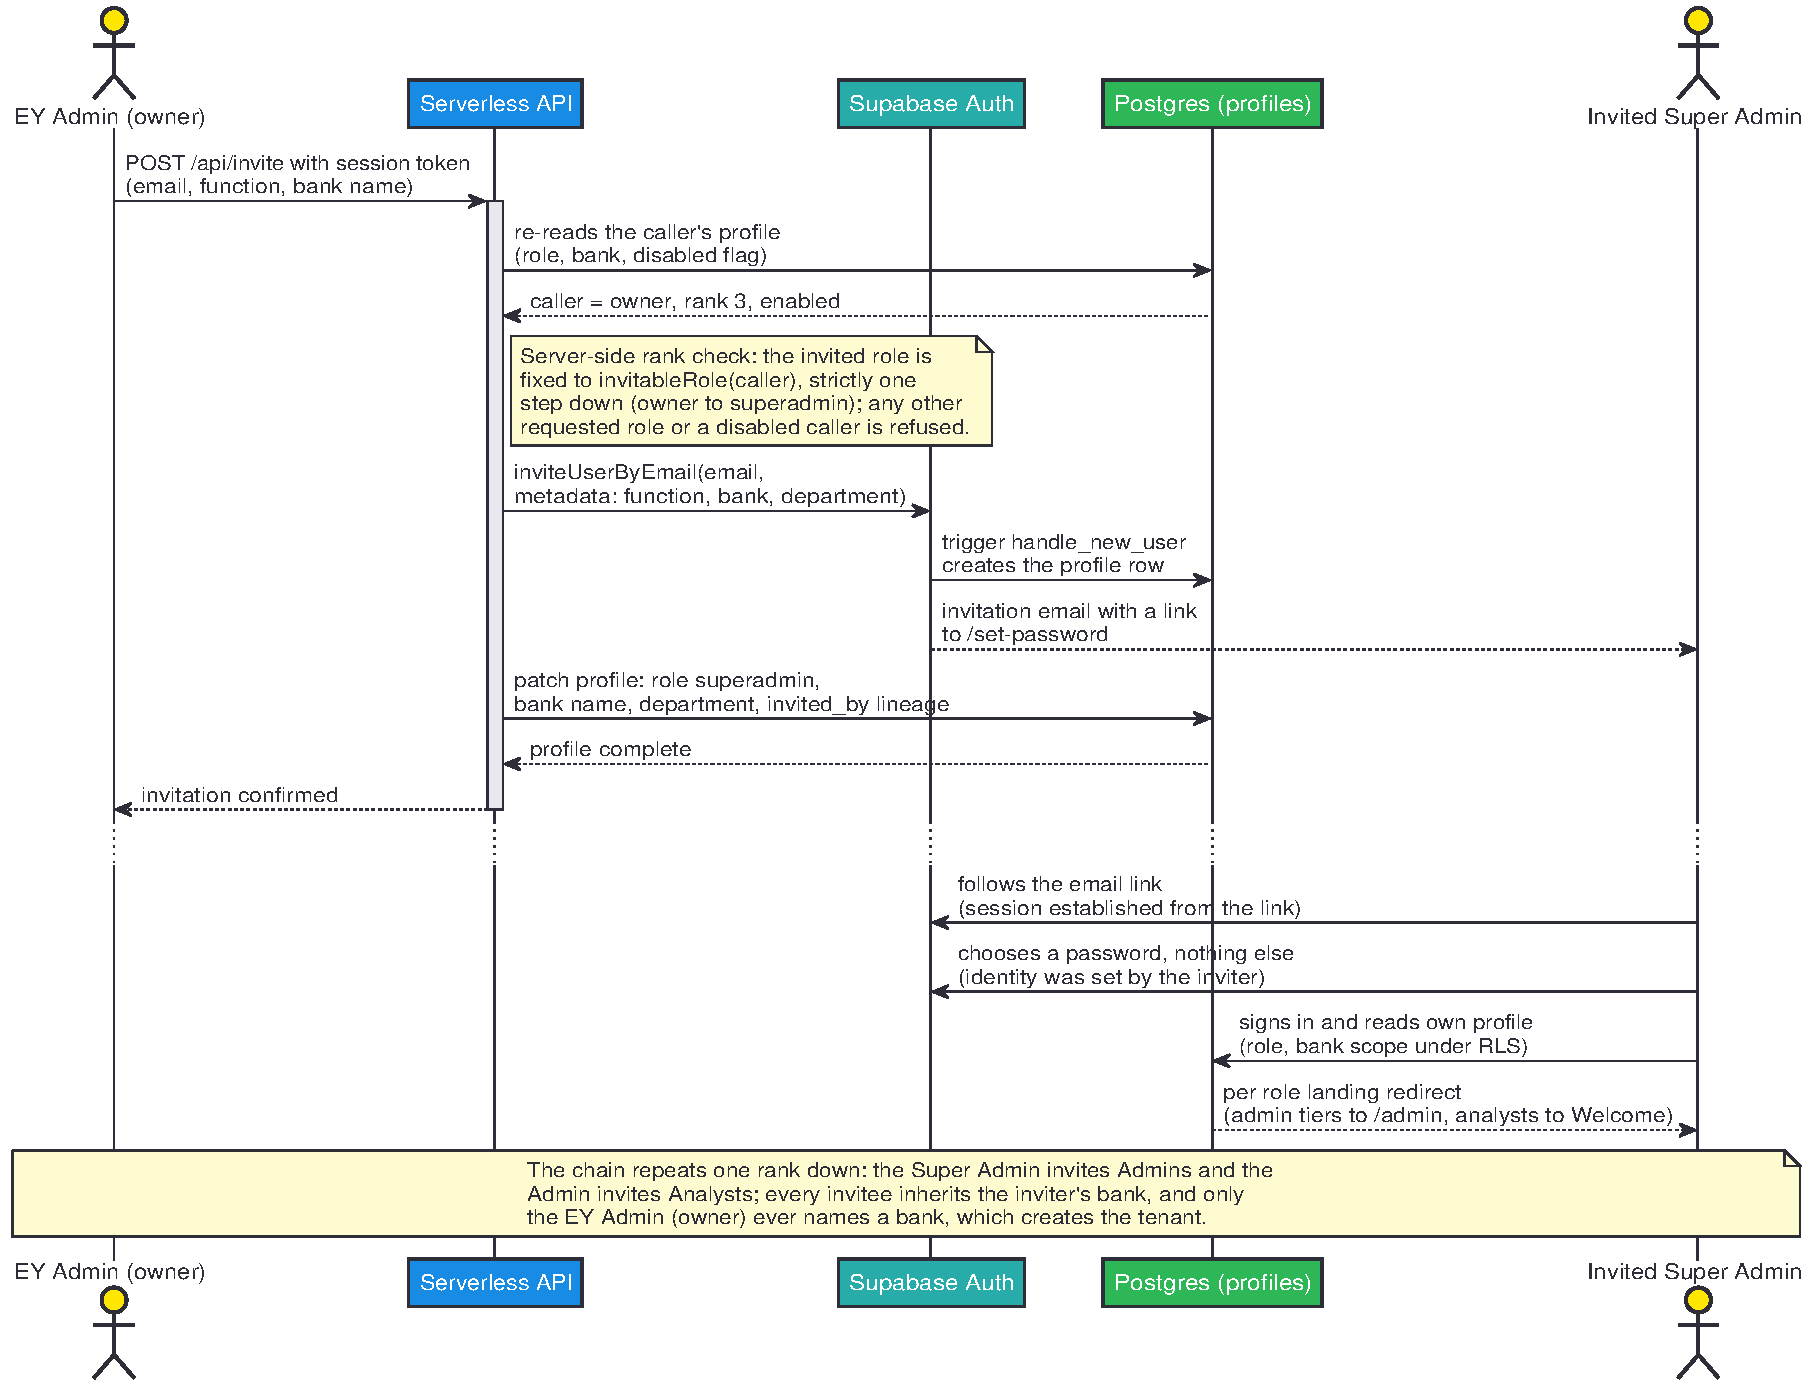
\includegraphics[width=\textwidth]{images/sequence-onboarding.pdf}
\caption{Sequence of the top-down invitation and onboarding chain}
\label{fig:sequence-onboarding}
\end{figure}

The third decision introduces departments and the group assessment. A bank's Super Admin or Admin maintains the bank's departments, with a one-click seed of a standard Tunisian set. A group assessment is one shared assessment per bank, with at most one open draft at a time, a rule enforced by a partial unique index in the database: the coordinator, an Admin or Super Admin, maps each dimension of the bank's questionnaire to exactly one department; each department's analysts fill only their assigned dimensions; the coordinator watches per-dimension progress and live scores; and finalization turns the draft into a single immutable submission for the bank. There is no per-contributor score: all contributors write into one shared answer map, one row per indicator with its author recorded, and dimensions that remain unanswered drop out of the Global Maturity Index through the standard weight renormalization of Iteration 2. The flow from department mapping to finalization is shown in Figure~\ref{fig:group-assessment-flow}.

\begin{figure}[H]
\centering
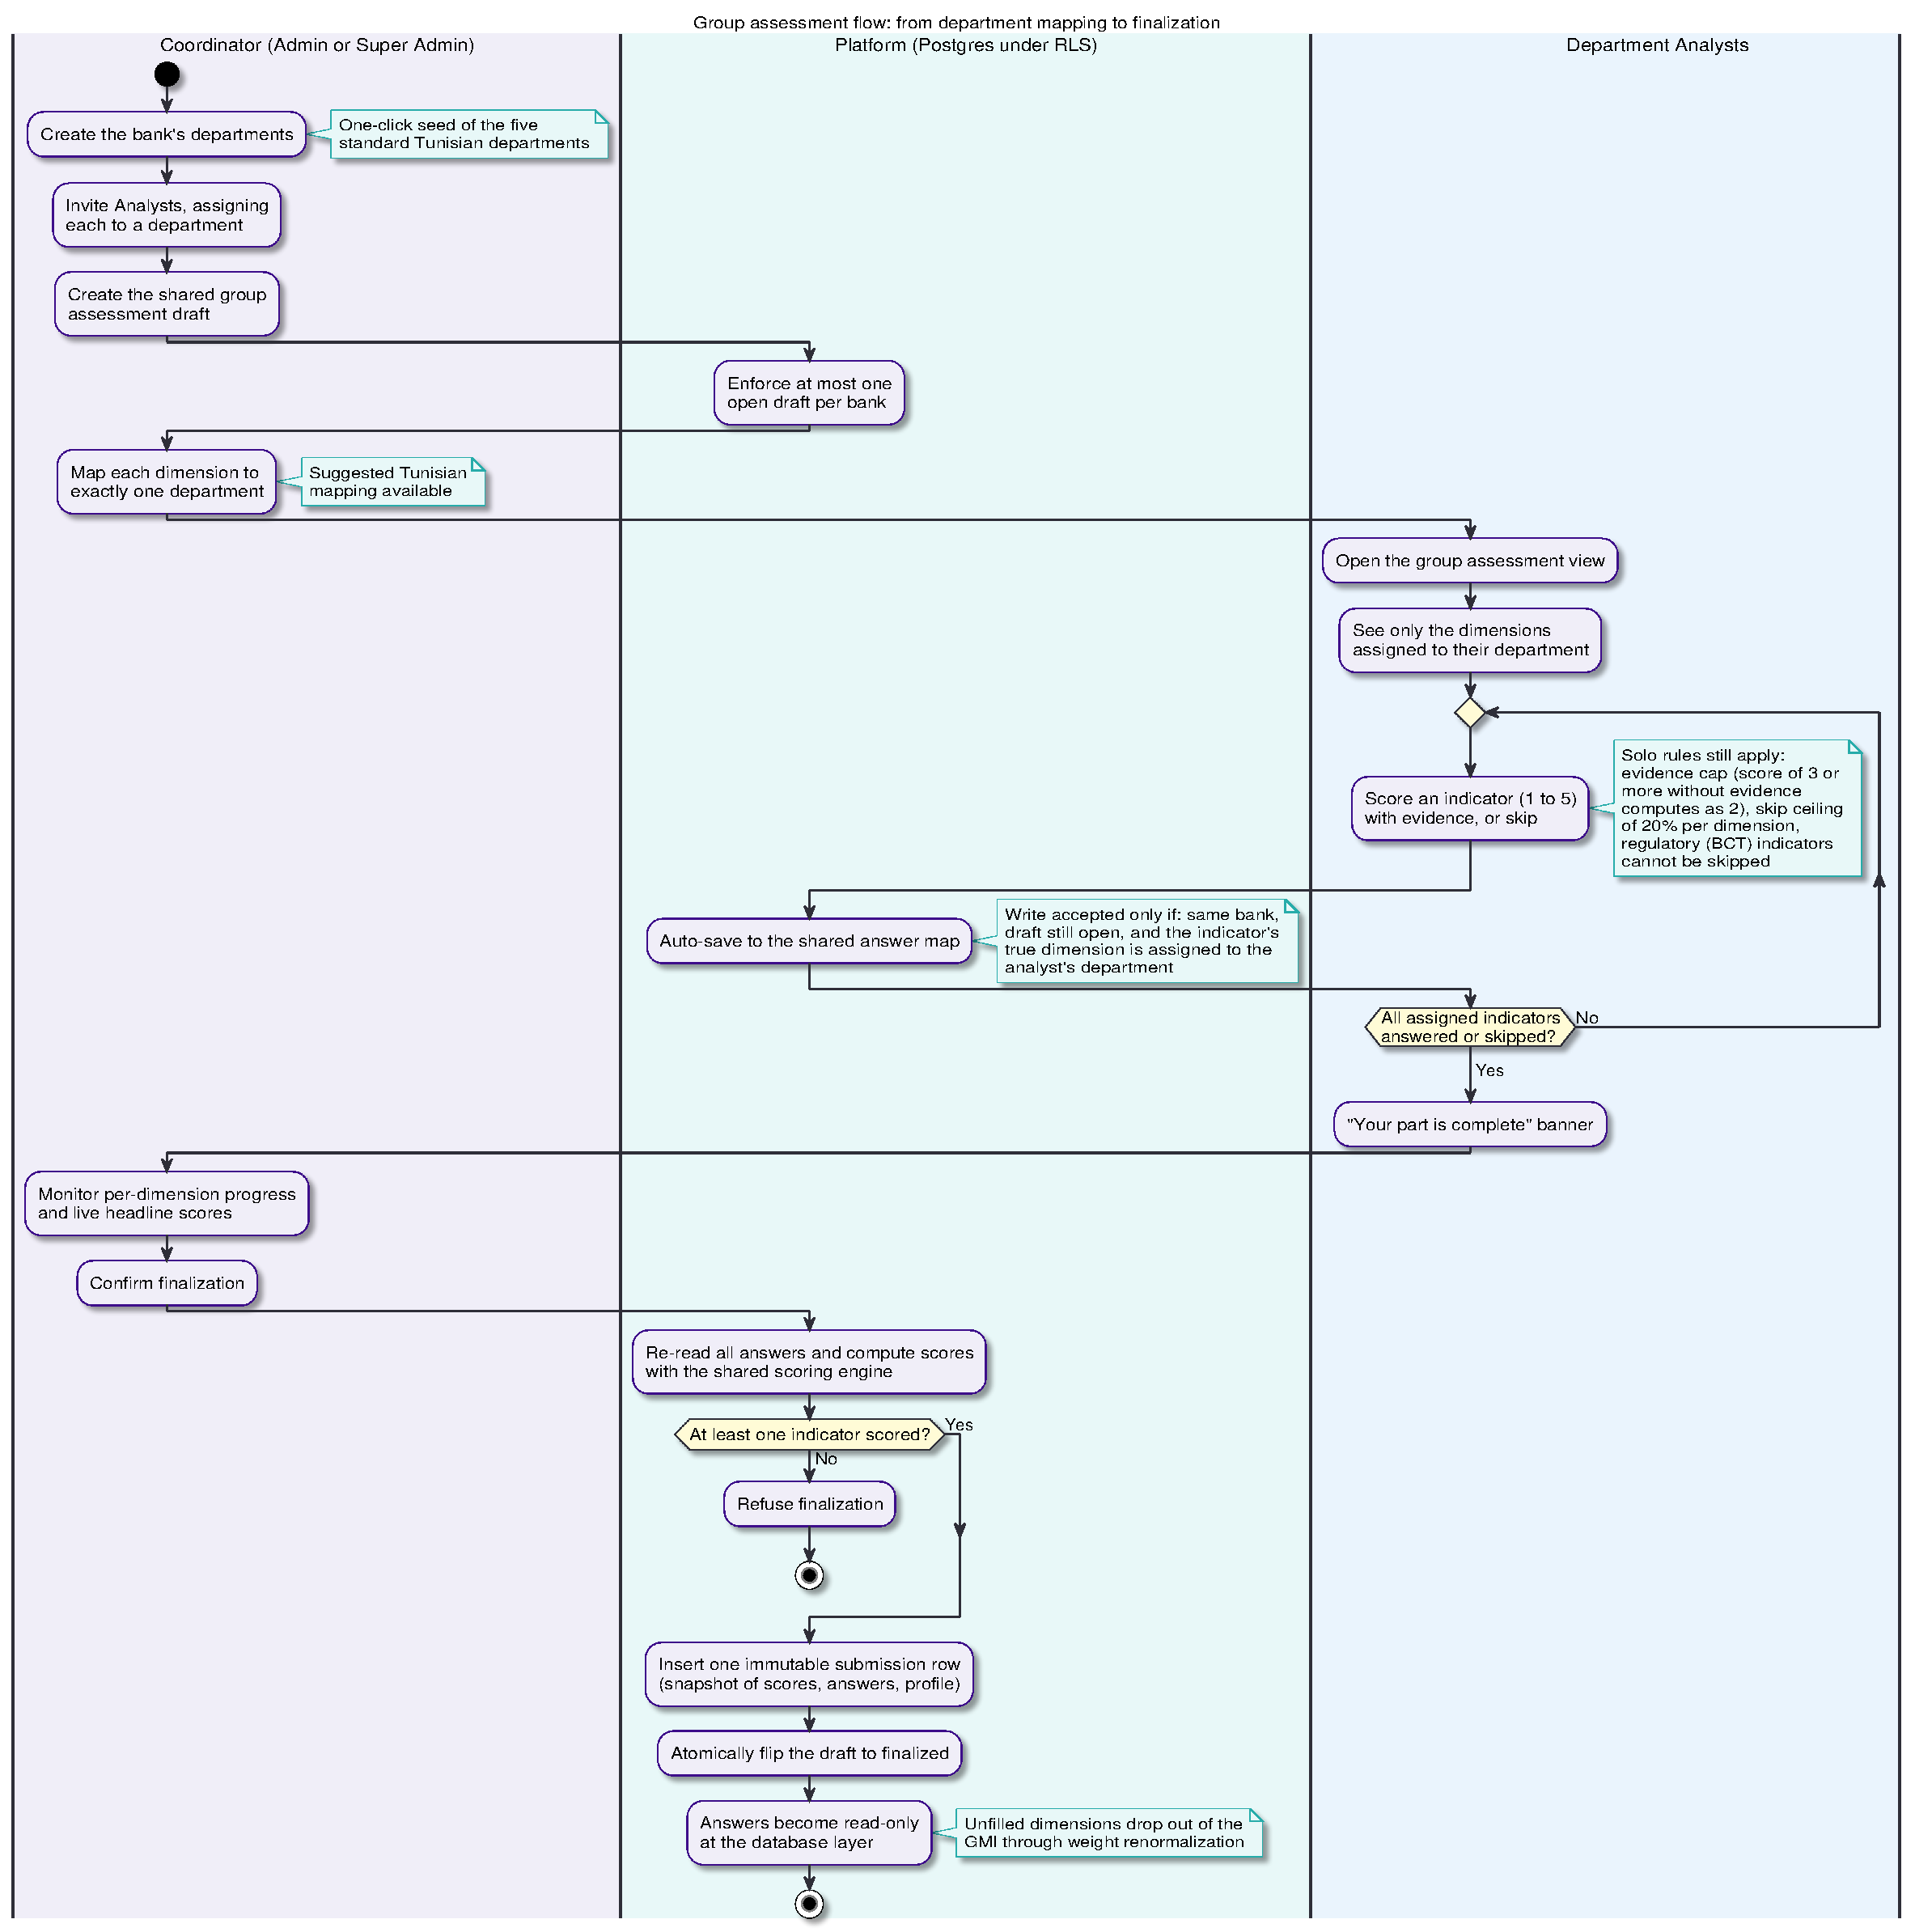
\includegraphics[width=\textwidth]{images/group-assessment-flow.pdf}
\caption{Group assessment flow from department mapping to finalization}
\label{fig:group-assessment-flow}
\end{figure}

The fourth decision turns the framework content into governed data without making the method negotiable. The 47 indicator framework of Iteration 1 is loaded as the EY master template, the reference instrument of the platform: the EY Admin maintains the master, each bank receives a bank copy cloned from it, and the bank's Admin may tailor that copy, adjusting dimension names, weights, descriptions, indicator questions, hints, five level rubrics, regulatory flags, and structure. Super Admins are deliberately read-only on content. Master edits seed future bank copies only; existing copies are frozen clones. Crucially, the scoring rules stay hard-coded and non-negotiable in every tenant: the evidence cap, the skip ceiling of 20\% per dimension rounded down, the non-skippable status of regulatory-flagged indicators, the compliance thresholds, namely an effective score of at least three with exposure rated low from eighty percent and medium from fifty, the five maturity bands, and the five level scale itself. In one sentence: the content became governed data; the method did not.

The fifth decision retains the solo assessment. Analysts keep the individual assessment path of Iteration 3, with in-progress answers still held locally in the browser and now bound to the signed-in account. Because browser local storage is plaintext scoped to a browser profile, this binding prevents the application from loading another signed-in user's draft into the interface, but it is not an encryption boundary: anyone with operating-system or developer-tools access to the same browser profile could still read the raw store directly. A completed solo assessment can additionally be submitted for review, which records an immutable submission row visible to the bank's administrators.

\subsubsection{Design Validation}

Two safeguards protect each bank's data: the database itself blocks any attempt to read another bank's records, and the privileged administrative actions re-check the user's role on the server on every request. The validation argument of this iteration is a two-layer enforcement argument, walked, as in the previous iterations, by tracing the worst case of each threat through the design before accepting it. The two layers are not two independent checks stacked over the same operation, and so are not defence-in-depth in the strict sense; they divide the work across two classes of operation. Row-level security in the database is the sole authoritative check for the ordinary read and write path, while the privileged service-role endpoints bypass row-level security by design, so for those operations the server code is the sole authoritative check rather than a second line behind the database.

\begin{sloppypar}
The first layer, authoritative for the ordinary data-access path that reads and writes take, is row-level security in the Postgres database itself. In plain terms, row-level security means that the database itself checks, on every single row it returns or accepts, that the reader or writer belongs to the same bank as that row, so tenant isolation does not depend on the application code remembering to filter. Every table policy funnels through a small set of security-definer helper functions, among them \texttt{is\_owner()}, \texttt{is\_admin()}, \texttt{is\_superadmin()}, \texttt{is\_bank\_admin()}, \texttt{is\_analyst()}, \texttt{my\_bank()}, and \texttt{my\_department()}, and the tenant isolation pattern is uniform across tables: a row is accessible when the caller is the EY Admin or when the row's bank name equals the caller's own bank. These helper functions read the caller's identity, role, and bank from the authenticated session established at login rather than from any value the client can set, so a tampered request cannot change who the caller is. The \texttt{profiles} table carries no client write policy at all, so the browser cannot write a role even while holding the public key.
\end{sloppypar}

The second layer is the small set of privileged serverless endpoints holding the service-role key, which bypasses row-level security by design; for these operations the authoritative authorization check is therefore not the database but the server code, which re-reads the caller's role and bank on every request. Each role-gated endpoint, covering invitations, role changes, account management, and department assignment, re-reads the caller's profile from the database on every request and never trusts a client-sent role; the self-service endpoint verifies the caller's session token but grants no role-dependent capability. Route guards exist in the client as well, but they are user experience only and carry no security weight; the design records this honestly rather than counting them as a defense.

\begin{sloppypar}
The self-escalation worst cases were each traced to a refusal. An invitation may only create the role exactly one rank below the caller, and any other requested role is refused. No user can change their own role at all through \texttt{/api/set-role}; a granted role and the target's current role must both be strictly below the caller's rank, and a caller other than the EY Admin is confined to their own bank. Disabling an account through \texttt{/api/manage-user} is reserved to the Super Admin tier and above and never applies to oneself. The self-service endpoint \texttt{/api/update-self} accepts only a whitelist of fields, the name, the language, the avatar, and the phone, and explicitly ignores any attempt to change the bank, because the bank name is the tenant identifier and is read-only in the application. Finally, disabled accounts are re-checked on the server on every role-gated call, so a revoked administrator holding a still-valid session token is cut off from the administrative endpoints immediately.
\end{sloppypar}

\begin{sloppypar}
Submissions were validated as immutable against modification. The \texttt{submissions} table has no update policy, so a written result cannot be altered in place: neither an analyst nor an administrator can change a submission once it has been recorded. Deletion is a distinct operation and is not blocked outright, but it is restricted to the owner of the row that submitted it and the bank's administrators; the insert policy compares the submission's bank name to the caller's own bank, so a submission cannot be forged into another tenant. The immutability claim is therefore precise: a recorded submission can never be edited, and it can be removed only by its submitting owner or a bank administrator. Adding append-only deletion protection, so that a finalized submission cannot be deleted at all, is noted as a further hardening step.
\end{sloppypar}

\begin{sloppypar}
The hardest case is the group answer path. An analyst's write to the shared draft in \texttt{assessment\_answers} is accepted only when four conditions hold at once: the caller is an analyst, the caller belongs to the same bank as the assessment, the assessment is still a draft, and the indicator's true dimension, looked up on the server rather than taken from the client, is assigned to the caller's department. A database trigger additionally overwrites the answer's dimension code and its author before the row is stored, so neither can be spoofed. Finalization flips the draft to finalized with an atomic conditional update; when two coordinators race, the loser deletes its own just-inserted submission row and reports that the assessment was already finalized; and a finalized assessment becomes read-only at the database layer.
\end{sloppypar}

Several of these rules were added by successive hardening migrations after design review of the policy chain, covering client-supplied dimension codes, submission bank forgery, and draft locking; the row-level security design was, in this sense, iteratively reviewed and hardened during development.

\subsubsection{Solution Implementation}

\begin{sloppypar}
The platform was implemented on Supabase, which provides the Postgres database holding all tenant data under row-level security, the authentication service handling email and password sign-in, invitation emails, and an optional phone-based step-up verification, and the file storage that holds user avatars under per-user write policies. The schema is built by an ordered chain of seventeen SQL migration files, and the final model comprises eight application tables: \texttt{profiles} (one row per account, carrying the role, the bank name as tenant key, the department, and the invitation lineage), \texttt{dimensions} and \texttt{indicators} (the per-bank questionnaire content, where the empty bank name denotes the EY master template), \texttt{submissions} (the immutable results of both solo submissions and group finalizations), \texttt{departments} (the bank's organization units), \texttt{assessments} (the shared group drafts, at most one open draft per bank through the partial unique index \texttt{assessments\_one\_open\_draft}), \texttt{assessment\_assignments} (the dimension to department map), and \texttt{assessment\_answers} (the shared per-indicator answers, each recording its author). The eight tables and the way the bank-name tenant key isolates each bank's data are summarized in Appendix~D.
\end{sloppypar}

\begin{sloppypar}
Above the database sits the serverless layer: five POST endpoints, \texttt{/api/invite}, \texttt{/api/set-role}, \texttt{/api/manage-user}, \texttt{/api/set-department}, and \texttt{/api/update-self}, each a thin handler delegating to a framework-agnostic core module, and the same core modules are mounted as middleware on the development server, so development and production share one code path. All five hold the service-role key on the server only. The deployment view of the platform, with the single-page application, the serverless endpoints, and Supabase under row-level security, is shown in Figure~\ref{fig:deployment}.
\end{sloppypar}

\begin{figure}[H]
\centering
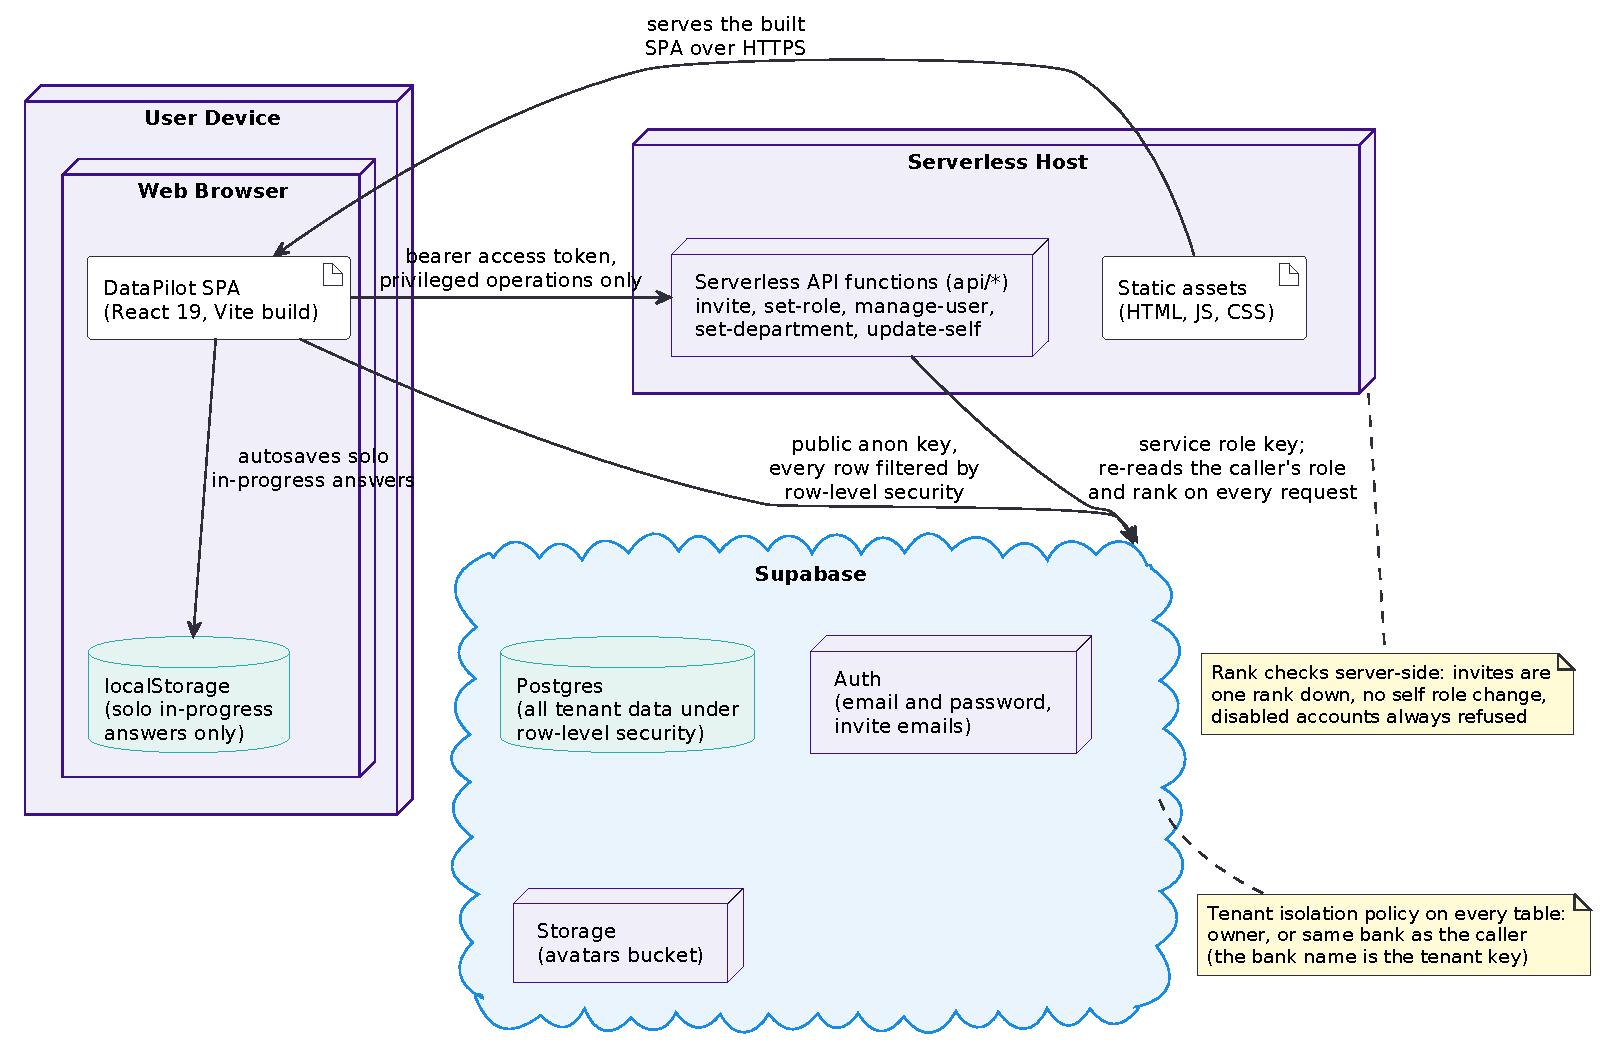
\includegraphics[width=0.75\textwidth]{images/deployment.pdf}
\caption{Deployment view of the DataPilot platform: single-page application, serverless endpoints, and Supabase under row-level security}
\label{fig:deployment}
\end{figure}

\begin{sloppypar}
On the client, the state layer grew from the single store of Iteration 3 to eight Zustand stores, one for each piece of state the platform keeps: login (the session, role, and identity, kept clean on account switch), the solo assessment (with the scoring engine unchanged), the group assessment, the questionnaire content (loaded through a fallback chain of the bank copy, then the EY master template, then the bundled defaults), the bank's users, its departments, its submissions, and the language preference.\footnote{The eight Zustand stores are, respectively, \texttt{useAuthStore} (login), \texttt{useAppStore} (solo assessment), \texttt{useAssessmentStore} (group assessment), \texttt{useContentStore} (questionnaire content), \texttt{useUsersStore}, \texttt{useDepartmentsStore}, \texttt{useSubmissionsStore}, and \texttt{useSettingsStore} (language).} The scoring engine was extracted into a pure-function module, \texttt{src/lib/scoring.js}, so that the group finalization computes scores identically to the solo path, and the shared \texttt{AssessmentRunner} component renders both the solo questionnaire and the group contributor view with the same rubric cards, evidence field, cap warning, and skip ceiling. The layered architecture of the platform, with the four front-end layers of Iteration 3 now resting on a backend layer, is shown in Figure~\ref{fig:architecture-layers}: solo in-progress answers persist in the browser storage, while submissions, group assessments, profiles, and questionnaire copies persist in Postgres under row-level security.
\end{sloppypar}

\begin{figure}[H]
\centering
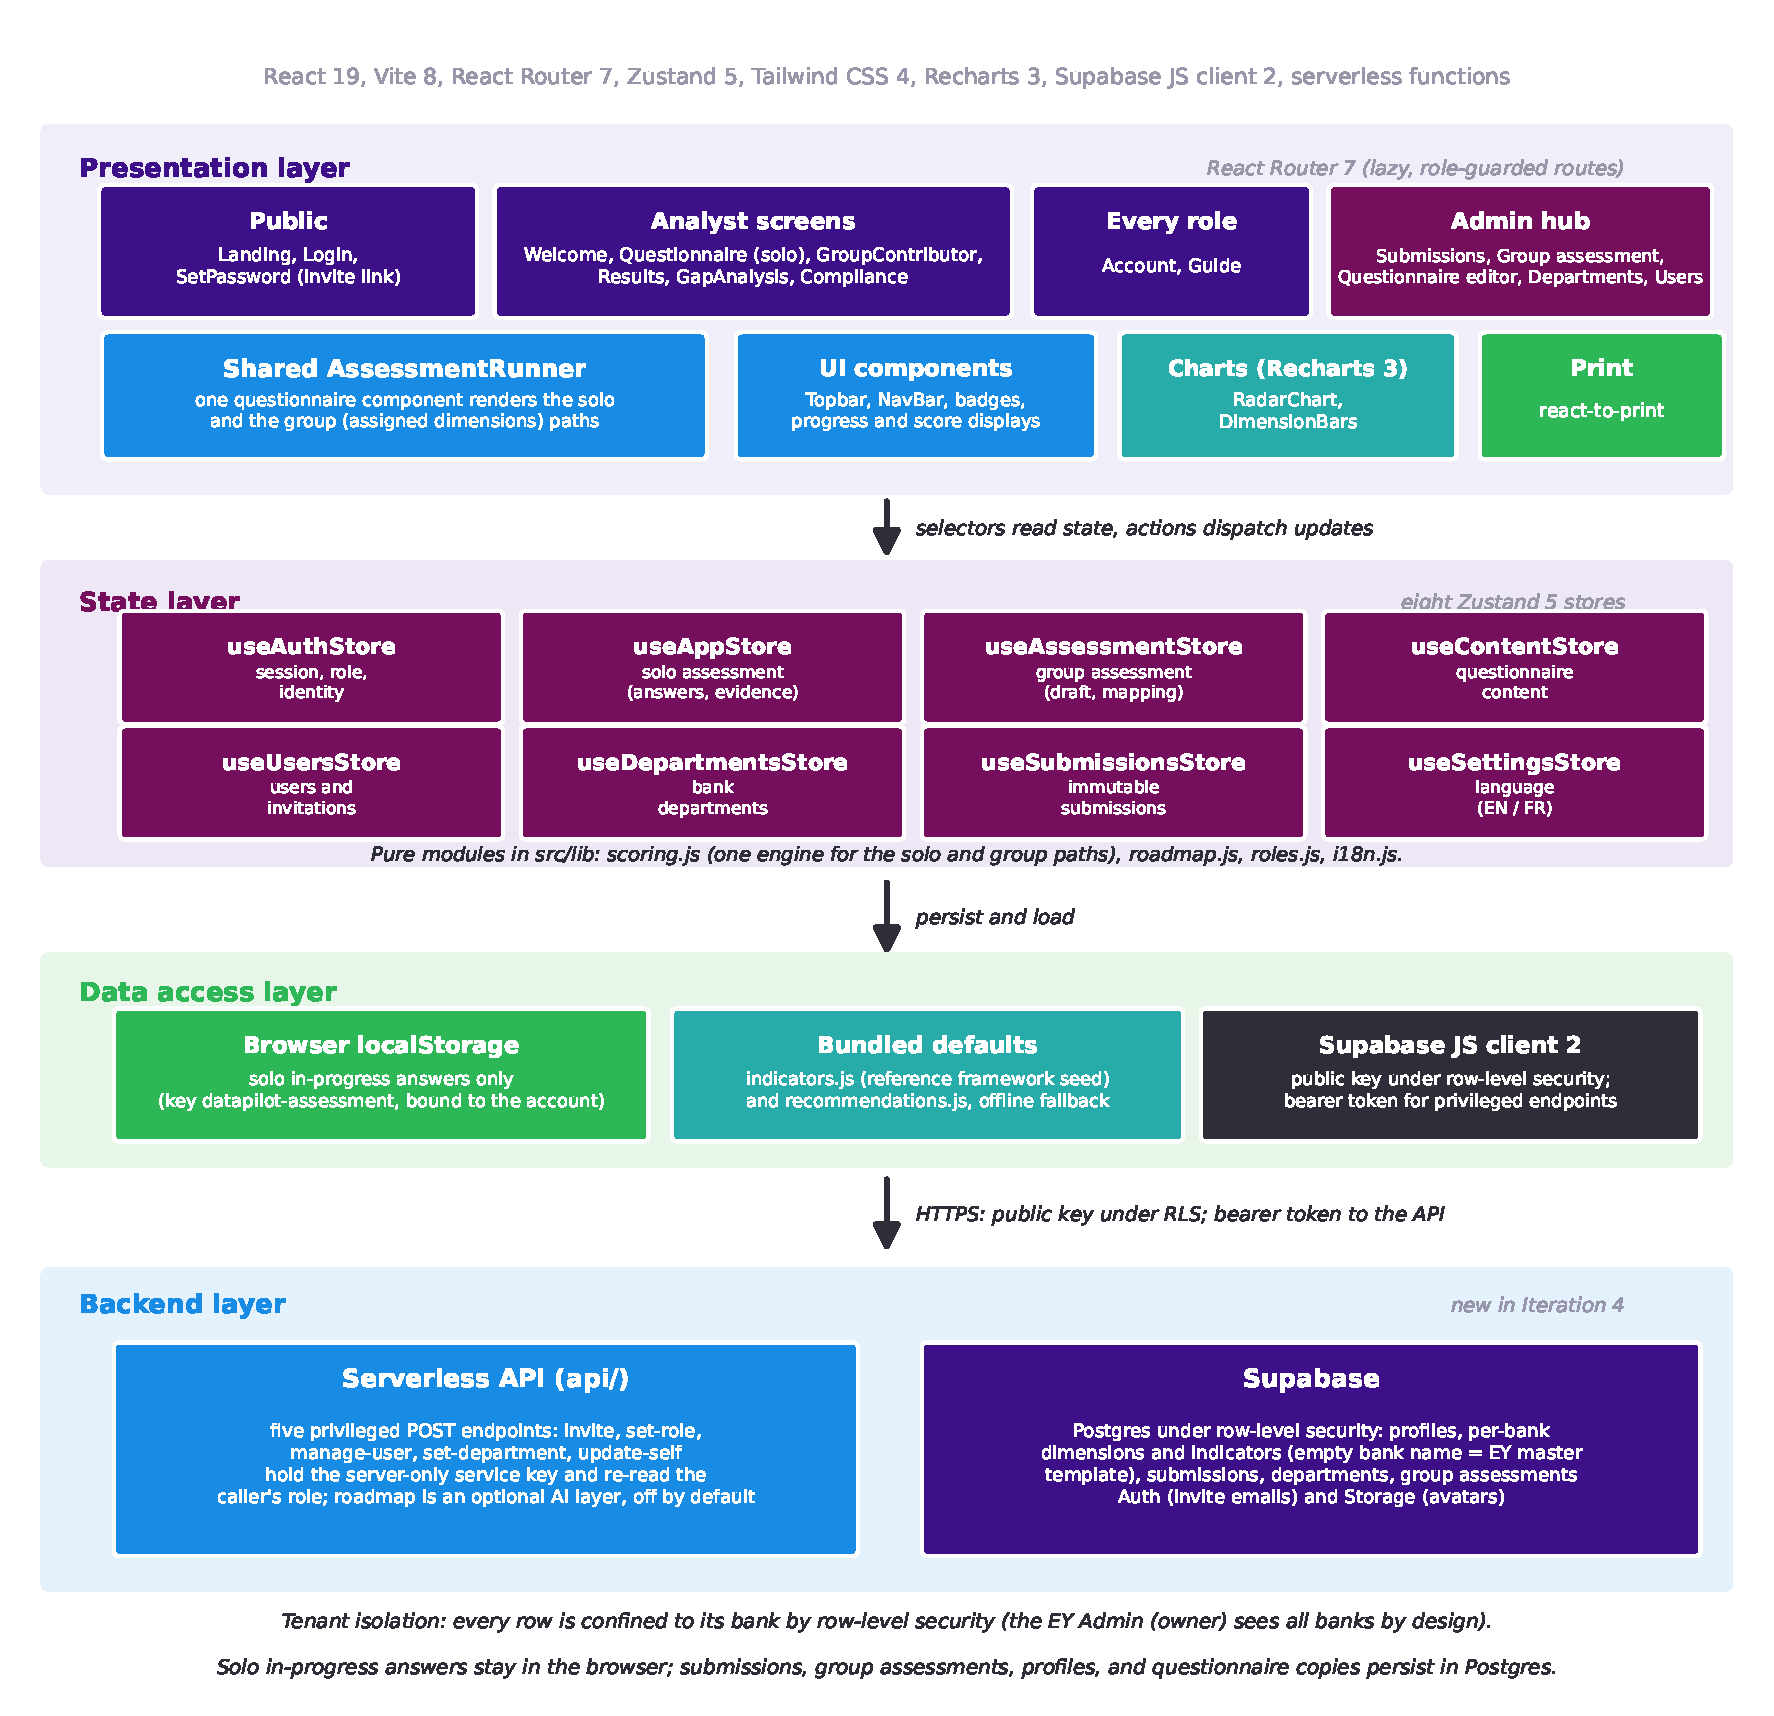
\includegraphics[width=0.85\textwidth]{images/architecture-layers.pdf}
\caption{Layered architecture of the DataPilot platform}
\label{fig:architecture-layers}
\end{figure}

The domain model grew accordingly. The assessment entities of Iteration 3, the dimensions, sub-dimensions, indicators, and answers, are joined by the platform entities: the profile with its role, bank name, department, and invitation lineage; the department; the assessment with its draft or finalized status and its target level; the assignment of a dimension to a department; the shared assessment answer recording its author; and the immutable submission snapshotting the scores, the answers, and the profile. The bank itself is not a table but the tenant key, a bank name carried by every scoped entity, with the empty key denoting the EY master template; the dimensions and indicators are per-bank content keyed by that name.

The screen set grew with the roles. A public landing page and the login screen front the platform; a set-password screen realizes invitation acceptance; the Welcome screen is role-aware and identifies the analyst from the account; an Account screen replaces the Profile page of Iteration 3, since identity is now account-driven and read-only where it is administered; a role-aware Guide serves as the handbook; a group contributor screen carries the analyst's part of a group assessment; and an administration hub gathers five role-filtered panels, Submissions, Group assessment, the Questionnaire editor, Departments, and Users and roles.

The account-driven identity is visible on the Welcome screen shown in Figure~\ref{fig:screen-welcome-account}: the name, function, and bank of the invited Analyst are sourced from the account and shown read-only, and the assessment date is set automatically.

\begin{figure}[H]
\centering
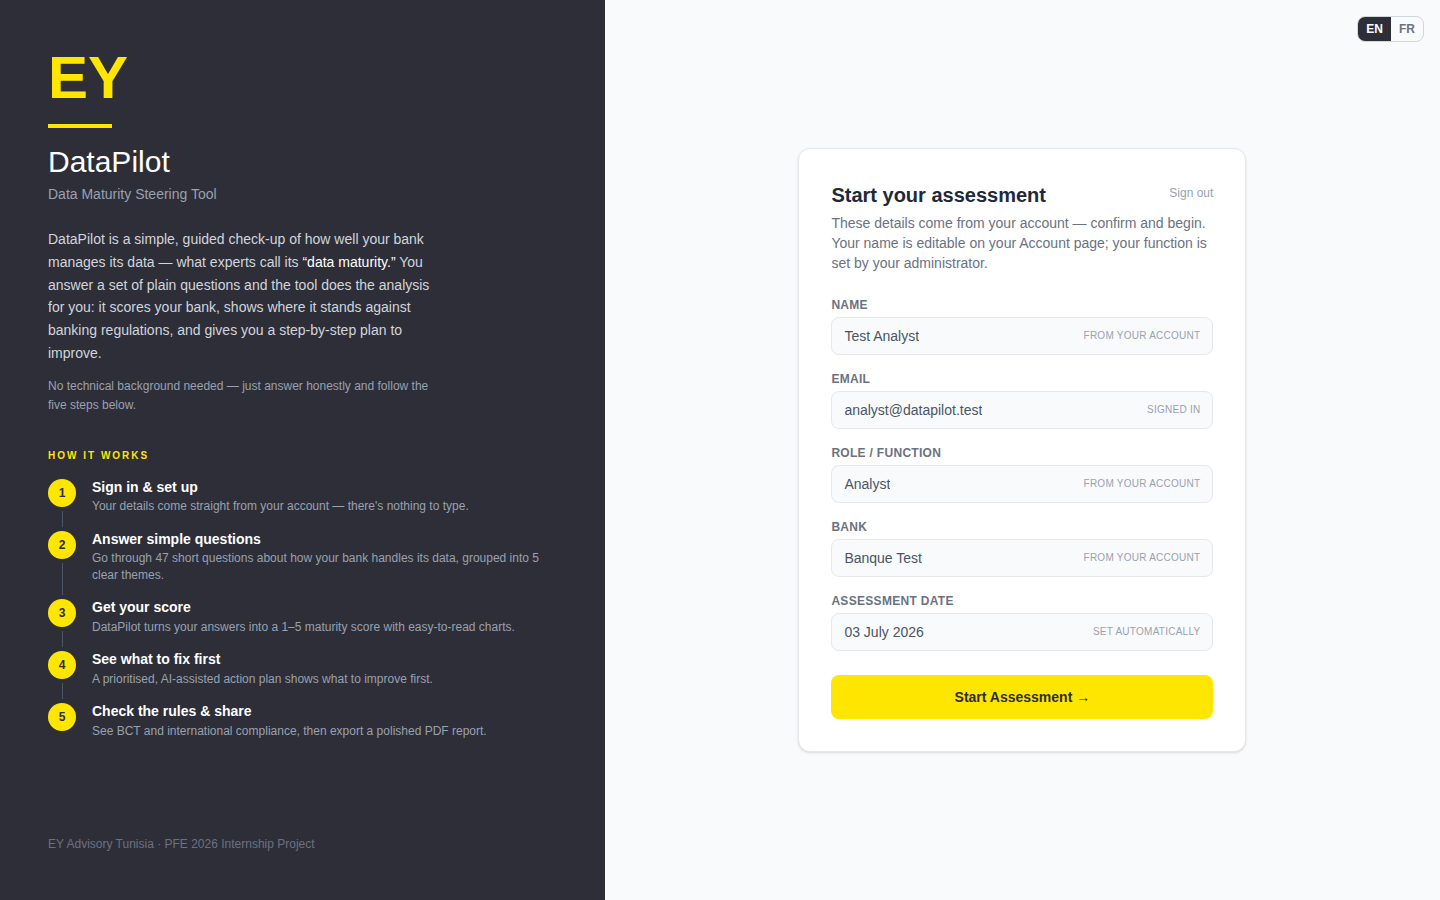
\includegraphics[width=0.85\textwidth]{images/screen-welcome-account.png}
\caption{Welcome screen of an invited Analyst: the identity block is sourced from the account and shown read-only}
\label{fig:screen-welcome-account}
\end{figure}

The application and its report chrome are fully bilingual in English and French through a hand-rolled dictionary and per-page copy objects, and the language preference follows the user across devices because it is mirrored to the profile. The questionnaire content itself is bank data and is deliberately not auto-translated.

The stack of Iteration 3 is unchanged, React 19, Vite 8, React Router 7, Zustand 5, Tailwind CSS 4, Recharts 3, and react-to-print 3, extended by the Supabase JavaScript client 2 and the serverless functions; the platform deploys as a static single-page application plus serverless functions on a Vercel-style host, with the environment split between public build-time keys and server-only secrets. Finally, the deterministic roadmap builder of Iteration 3 is unchanged, so the improvement actions remain generated in full from the stored recommendations rather than from any external service; an AI-assisted rewriting of these actions was considered but deferred to future work for the data-residency reasons discussed in the conclusion.

The running platform is shown in Figures~\ref{fig:screen-admin-users} through~\ref{fig:screen-group-contributor}, captured from the application executing against a locally provisioned Supabase backend, migrated with the full schema chain and seeded with the demonstration tenant used by the evaluation below. Figure~\ref{fig:screen-admin-users} shows the administration area as the Admin of the demonstration bank sees it: the Users and roles panel lists the bank's members with their roles and account status, and the invitation form offers exactly one invitable role, an Analyst, which is the one-step-down rule surfaced in the interface, with an optional department whose absence routes the invitee to a solo assessment. Figure~\ref{fig:screen-admin-group} shows the group assessment coordination panel, with each of the five dimensions assigned to its owning department, the per-dimension progress expressed over its indicator count, and the finalize action that will snapshot the completed assessment into an immutable submission. Figure~\ref{fig:screen-group-contributor} shows the same assessment from the contributor's side: the governance department's analyst is presented only with dimension D1 and its twelve indicators across three sub-dimensions, the scoring rules panel restates the evidence cap, the regulatory lock, and the skip ceiling of the dimension, and the Results, Gap Analysis, and Compliance views remain locked until the assessment completes. The running application also carries a clearly labelled demonstration control, a top-bar toggle that auto-fills the solo questionnaire with random test scores for walkthroughs; its random fill never survives a page reload, since the persisted state keeps only the user's real answers, and none of the evaluation scenarios reported here used it.

\begin{figure}[H]
\centering
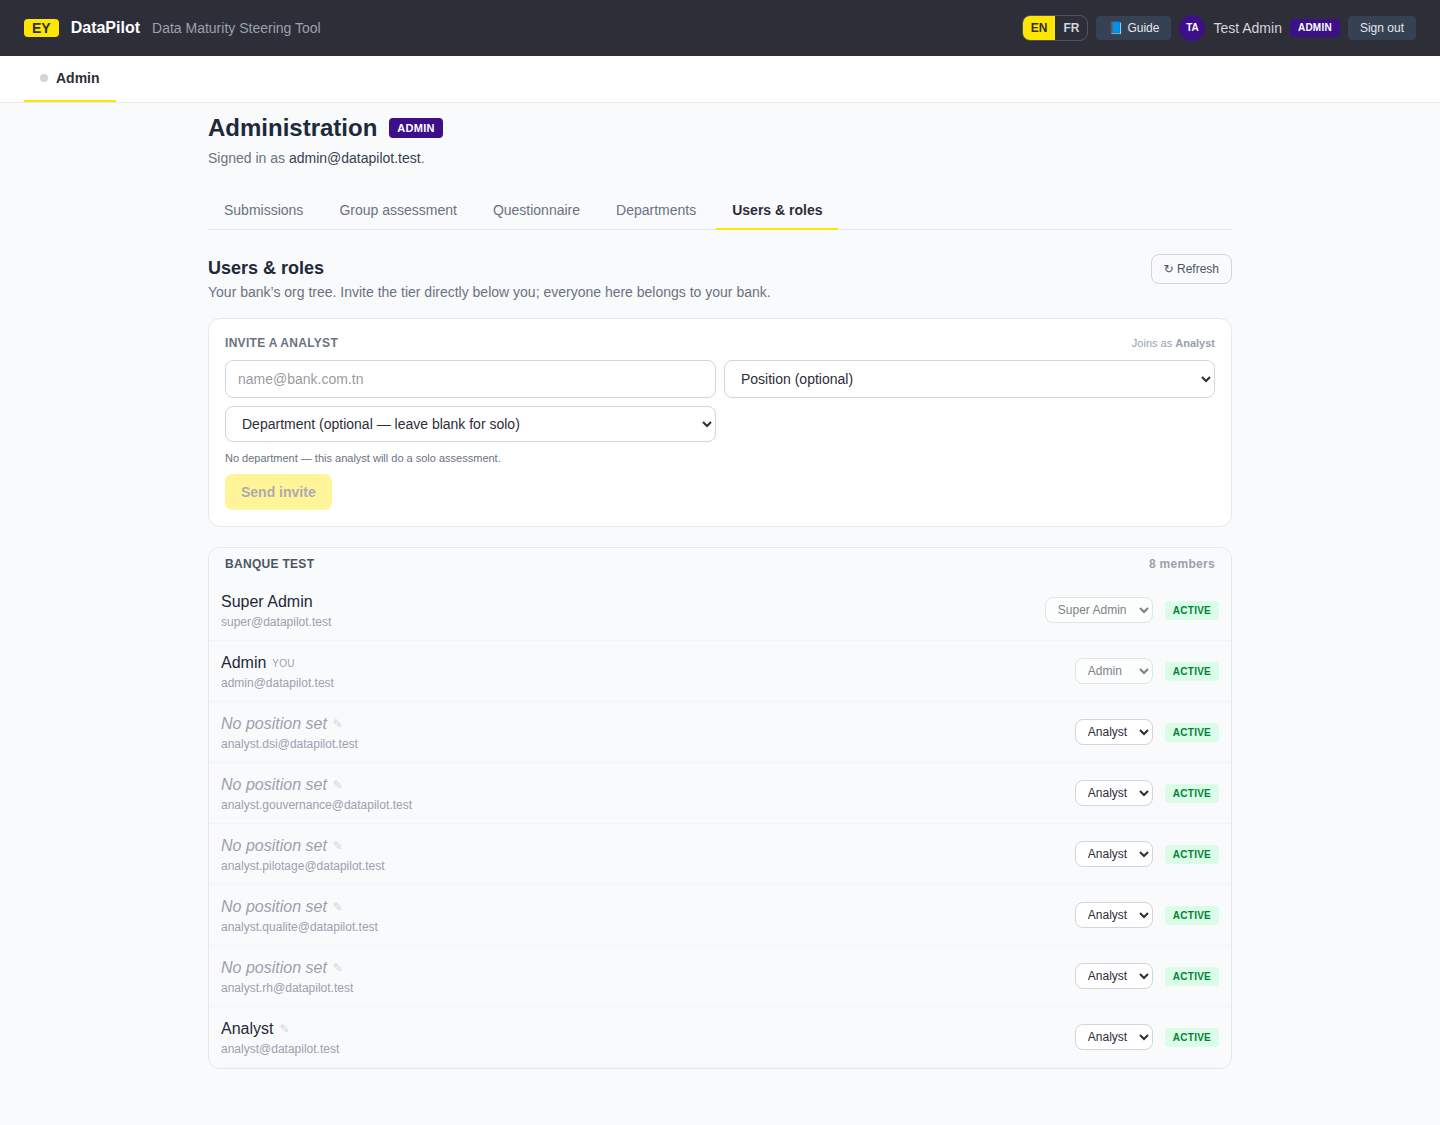
\includegraphics[width=0.92\textwidth]{images/screen-admin-users.png}
\caption{Users and roles panel of the bank Admin, with the one-step-down invitation form, captured from the running platform}
\label{fig:screen-admin-users}
\end{figure}

\begin{figure}[H]
\centering
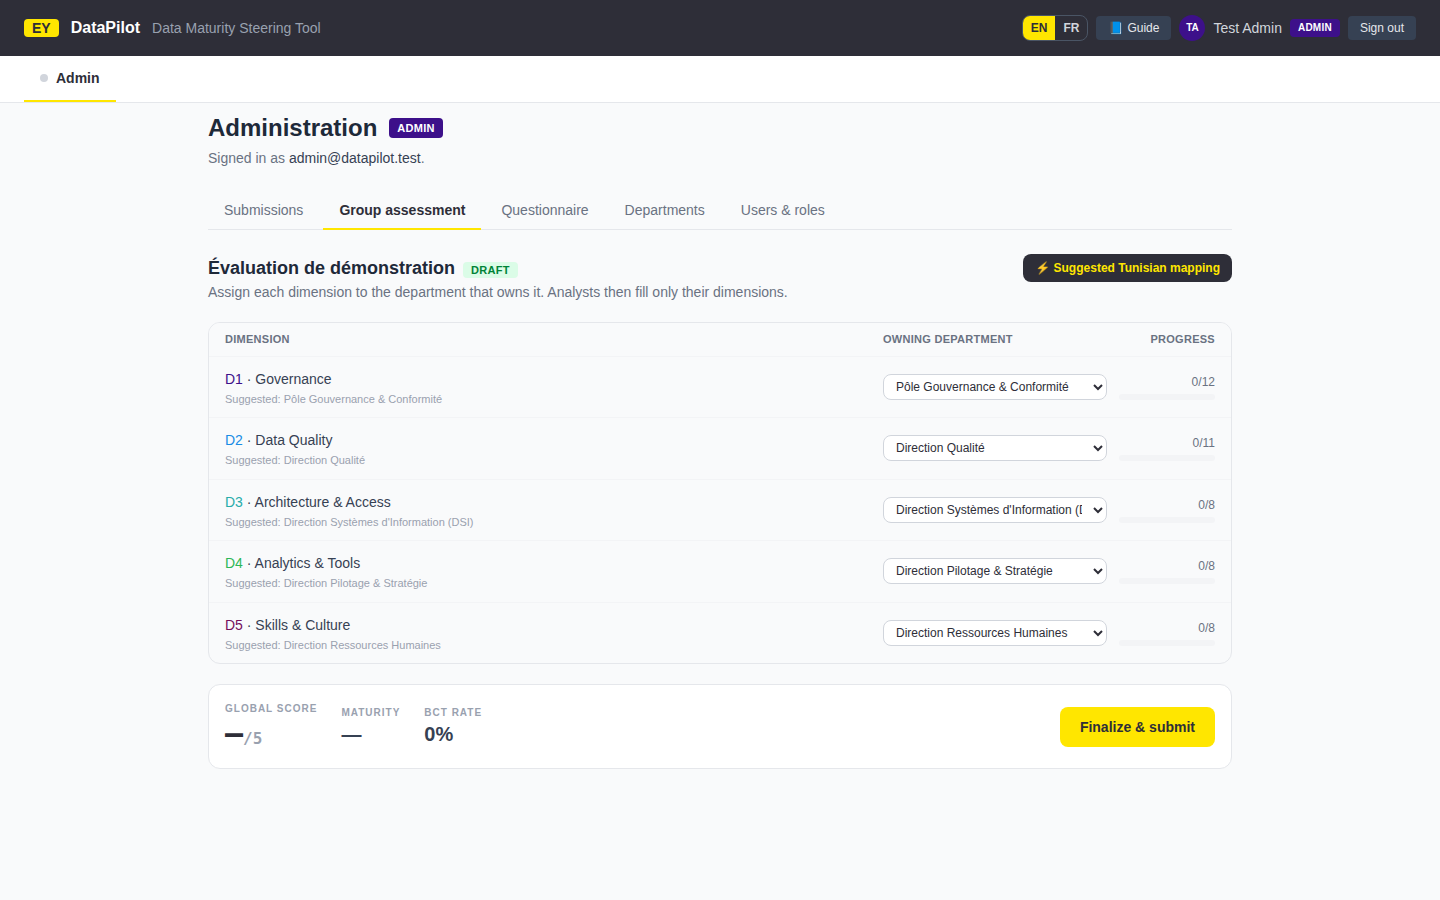
\includegraphics[width=0.92\textwidth]{images/screen-admin-group.png}
\caption{Group assessment coordination panel: dimensions mapped to owning departments, per-dimension progress, and the finalize action}
\label{fig:screen-admin-group}
\end{figure}

\begin{figure}[H]
\centering
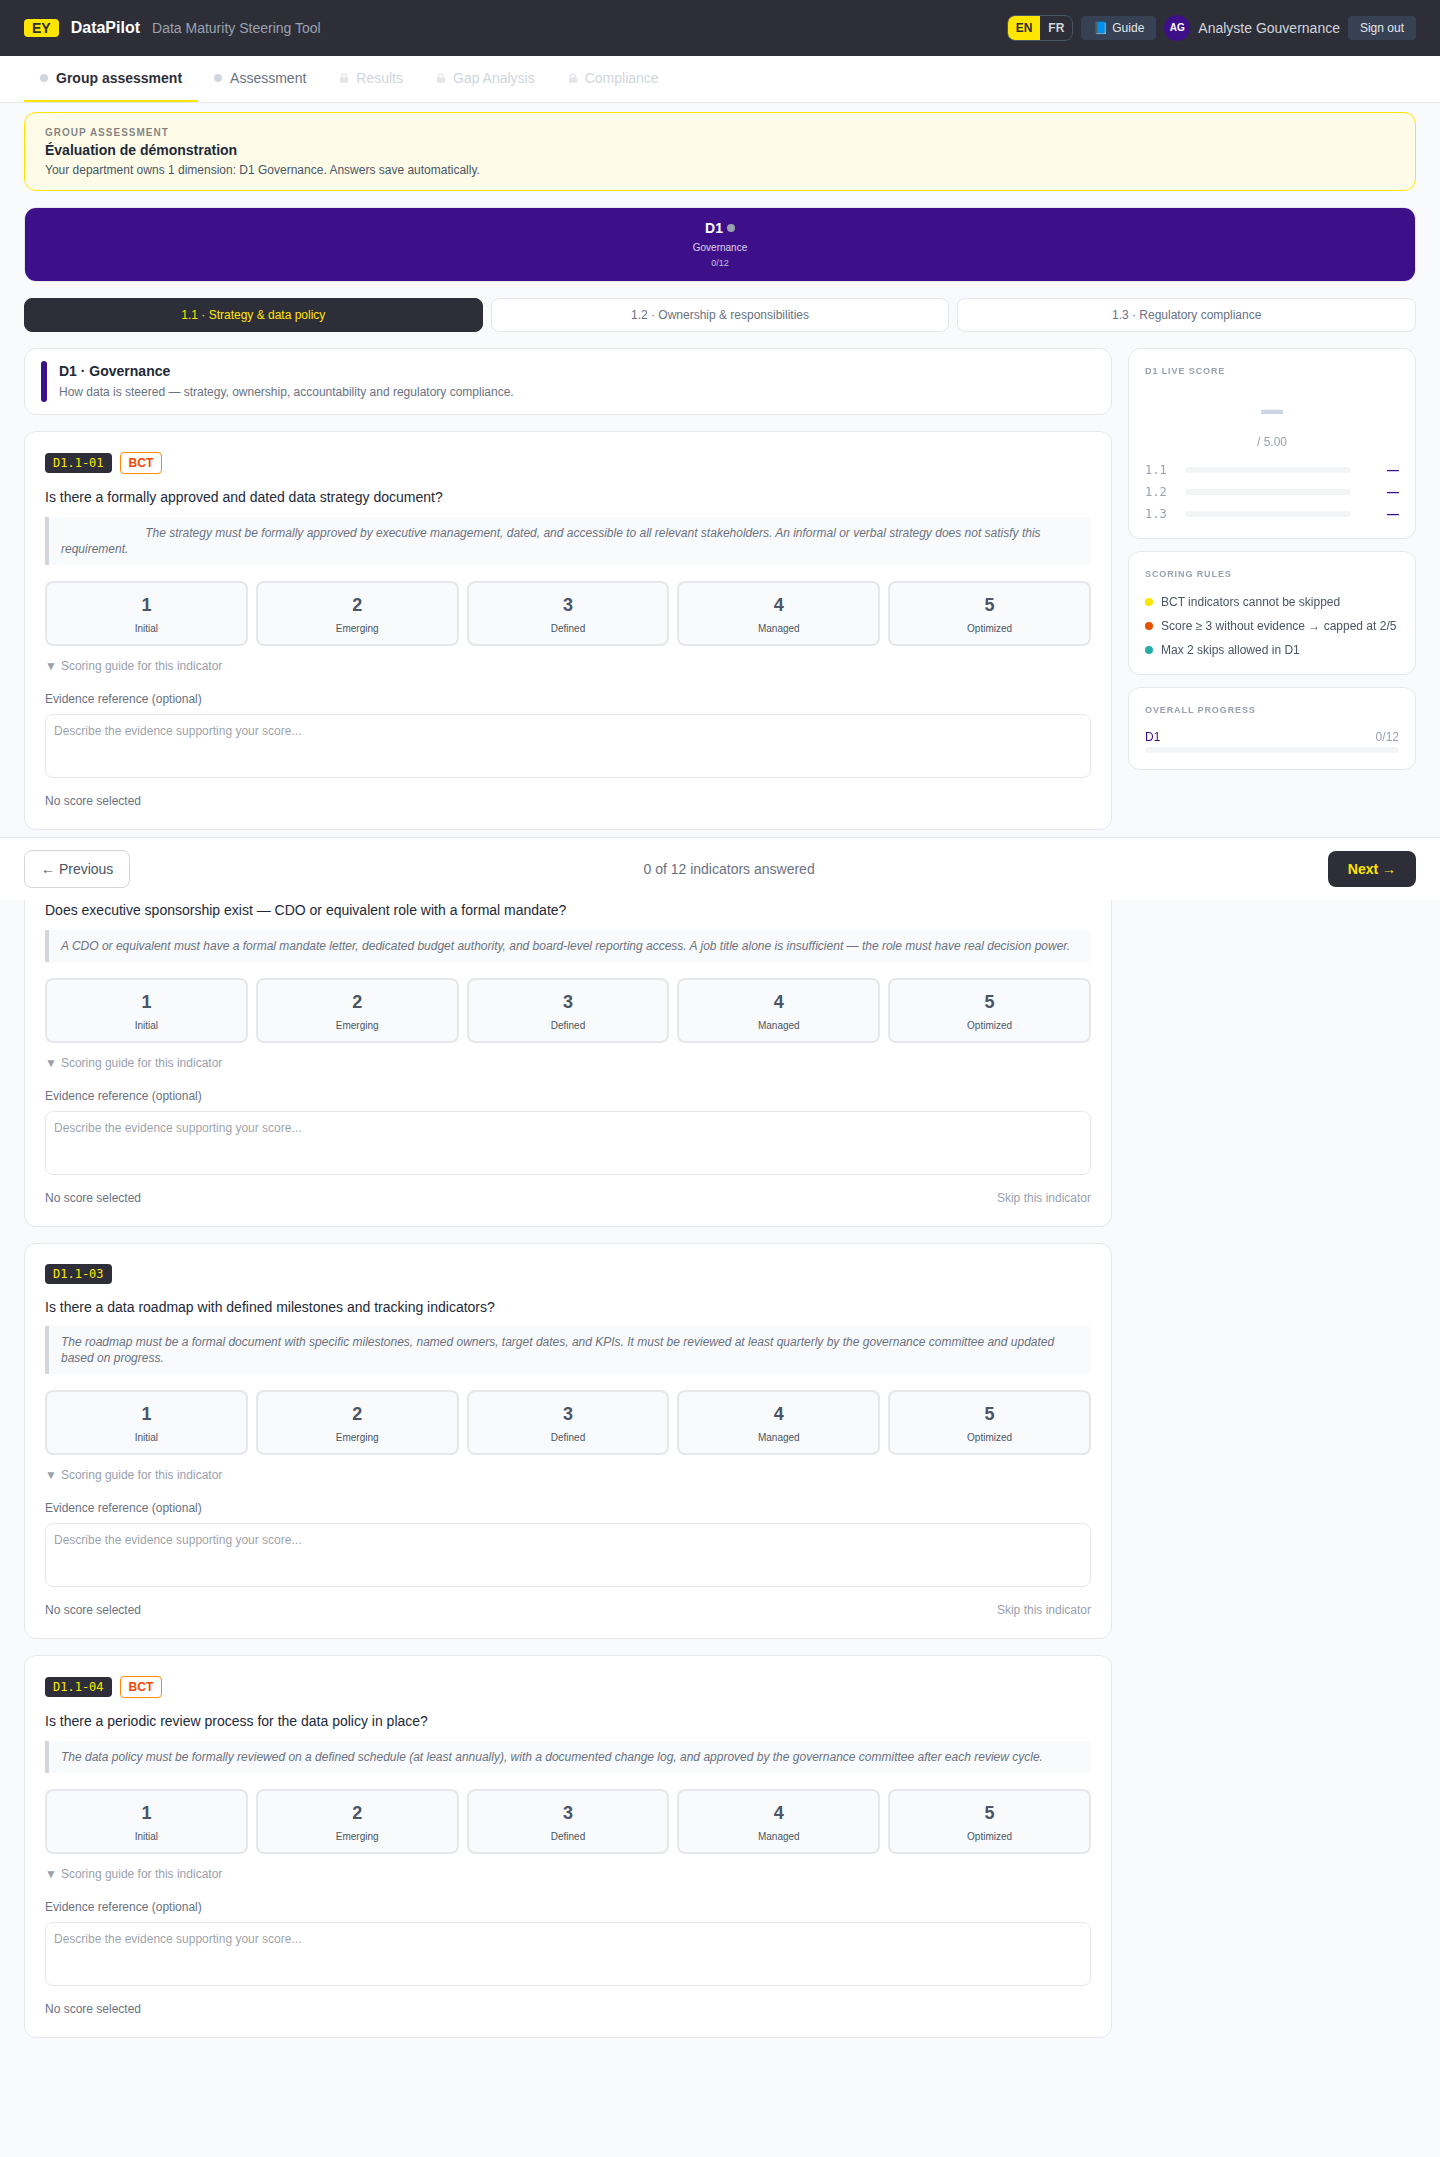
\includegraphics[width=0.6\textwidth]{images/screen-group-contributor.png}
\caption{Group contributor view: the governance department's analyst sees only dimension D1, with the scoring rules panel and the locked result views}
\label{fig:screen-group-contributor}
\end{figure}

Figure~\ref{fig:screen-admin-questionnaire} completes the administrator's view with the Questionnaire tab: a bank that has not yet tailored its content is offered a single action, creating the bank's own private copy from the EY master template, which is the content governance model of the fourth design decision surfaced in the interface.

\begin{figure}[H]
\centering
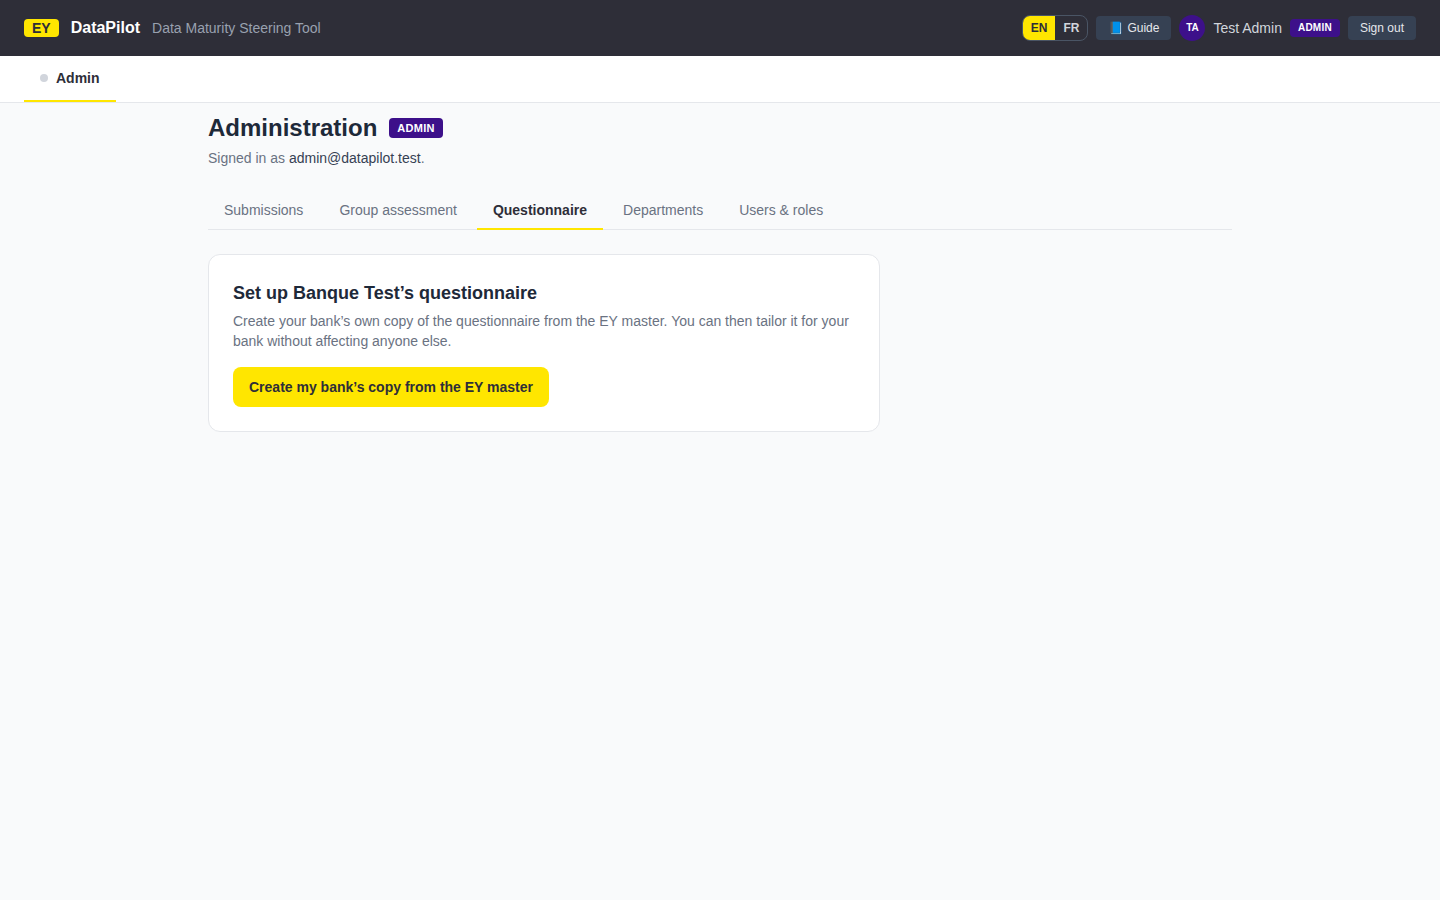
\includegraphics[width=0.92\textwidth]{images/screen-admin-questionnaire.png}
\caption{Questionnaire tab of the bank Admin before tailoring: the bank copy is created from the EY master template}
\label{fig:screen-admin-questionnaire}
\end{figure}

Figure~\ref{fig:screen-owner-admin} shows the same administration hub as the EY Admin (owner) sees it: only the Submissions, Questionnaire, and Users and roles tabs are offered, because the owner has no bank of its own and therefore no departments or group assessment to run, and the questionnaire it edits is the EY master template.

\begin{figure}[H]
\centering
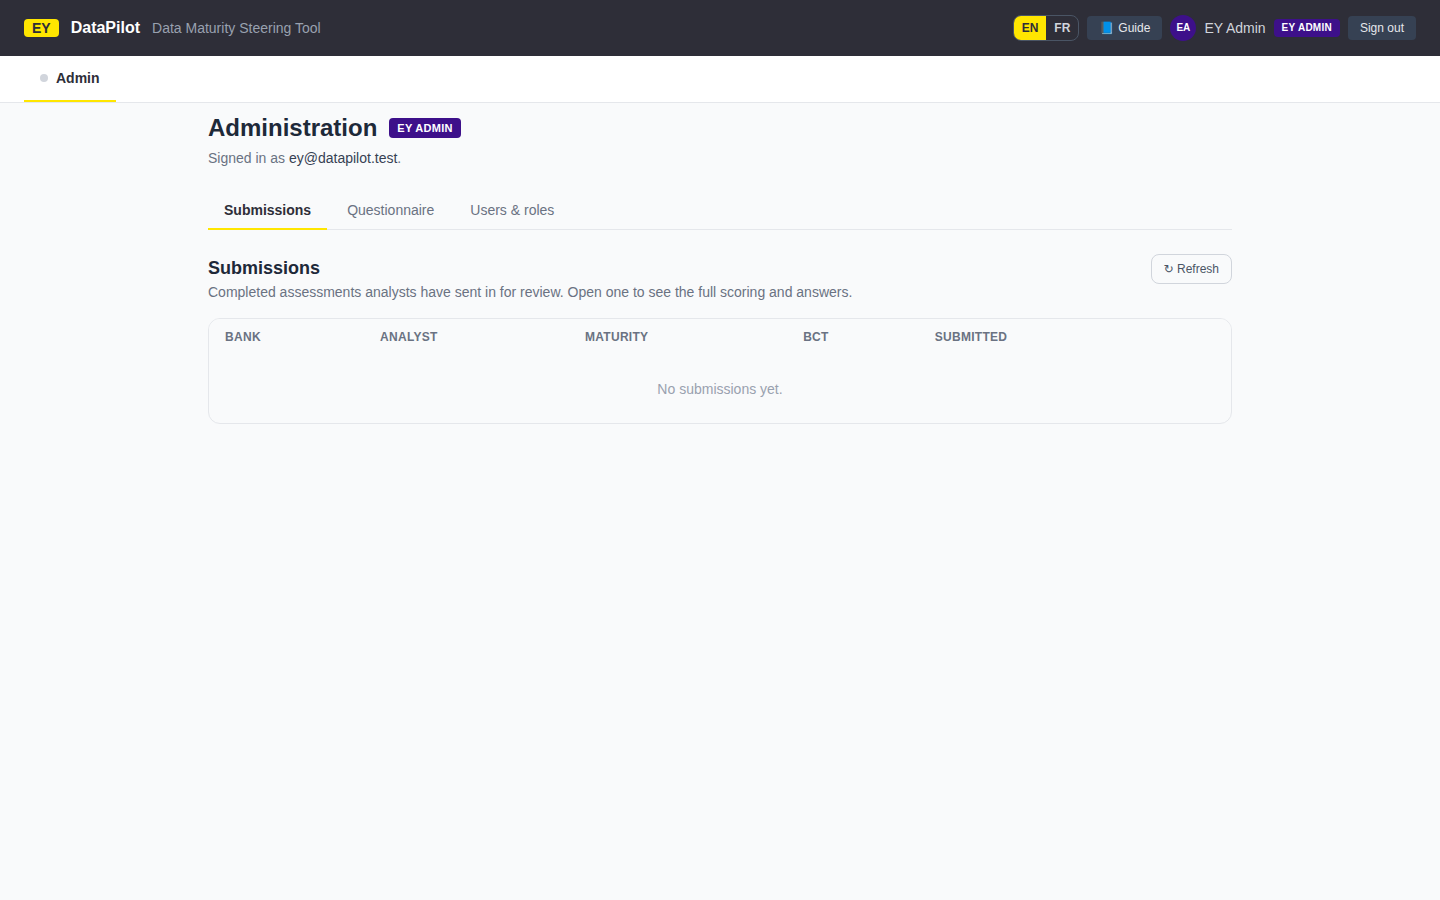
\includegraphics[width=0.92\textwidth]{images/screen-owner-admin.png}
\caption{Administration hub as the EY Admin (owner) sees it, with the role-filtered tab set and no bank-scoped panels}
\label{fig:screen-owner-admin}
\end{figure}

\subsubsection{Solution Evaluation}

As in Iteration 3, the evaluation consists of functional testing on simulated data, now grounded in a seeded demonstration scenario: a demonstration tenant, Banque Test, with seeded Super Admin, Admin, and Analyst accounts, five standard Tunisian departments, and a demonstration group assessment mapping the five dimensions to those departments, covering governance, quality, information technology, steering, and human resources. Five named, reproducible behaviors carry the evidence, mirroring the evaluation style of Iteration 3.

First, role gates refused. An Analyst requesting the administration area is redirected away; an Admin attempting to invite anything other than an Analyst is refused by the server; a user attempting to change their own role is refused; and a Super Admin cannot edit the questionnaire, which is read-only for that role by design, enforced at the database layer, with the editor tab not even offered in the interface.

Second, cross-tenant reads blocked by row-level security. Signed in as one bank's Admin, queries for another bank's profiles, submissions, or questionnaire copy return no rows; the EY Admin, by design, sees all banks.

Third, the invitation chain walked top-down. The EY Admin invites a Super Admin naming the bank; the invitee sets only a password and lands in the correct bank with the correct role; the same holds one rank down at each level; and a client-tampered role or bank in the invitation request is ignored or refused.

Fourth, the group assessment end to end. Dimensions are mapped to departments, including through the one-click suggested Tunisian mapping; an analyst sees only their department's dimensions; an attempted write to an unassigned dimension is rejected at the database layer; and the evidence cap, the skip ceiling, and the non-skippable regulatory indicators behave exactly as in the solo path.

Fifth, finalization locks the answers. After the coordinator finalizes, a contributor's further write is refused at the database layer, the assessment renders read-only, and exactly one immutable submission row exists for the bank; a second concurrent finalization attempt reports that the assessment was already finalized.

Beyond the local demonstration environment, the platform is deployed on a production Supabase instance, and a read-only inspection of that instance corroborates the implementation claims of this iteration. The production schema carries the same eight tables with row-level security enabled on every one of them, the security helper functions and the single-open-draft index are present, and all four roles of the hierarchy are populated across nineteen accounts, with one bank tenant, its five departments, and two assessments in progress at the time of inspection. The content model behaves exactly as designed: the EY master template and the bank's copy each hold the five dimensions with the canonical weights of 25/20/20/20/15 and the 47 indicators, of which thirteen carry the regulatory flag, so the reference framework of Iteration 1 is reproduced identically in the template and in the tenant copy. No finalized submission existed at the time of inspection, which is consistent with the evaluation boundary stated below.

The limitations of this evaluation are recorded honestly. It is scenario-based on seeded demonstration data, not a production pilot with real banks, and there is still no automated test suite. The tenant key is a free-text bank name, so a typo at Super Admin invitation would create a separate tenant. Master template edits do not propagate to existing bank copies, which are frozen clones whose re-synchronization is manual. Reviewing an old submission against a since-edited questionnaire can show mismatched labels, which is precisely why submissions store computed snapshots, so that the recorded numbers remain intact. And solo in-progress answers still live in the analyst's browser until submission. These limitations are recorded for the future work.

\subsection{Use Case Specifications}

The full set of interactions supported by the platform, across its four roles and the two Iteration~3 actors, is captured in the use case diagram of Figure~\ref{fig:usecase}, which the specifications below detail one use case at a time.

\begin{figure}[p]
\centering
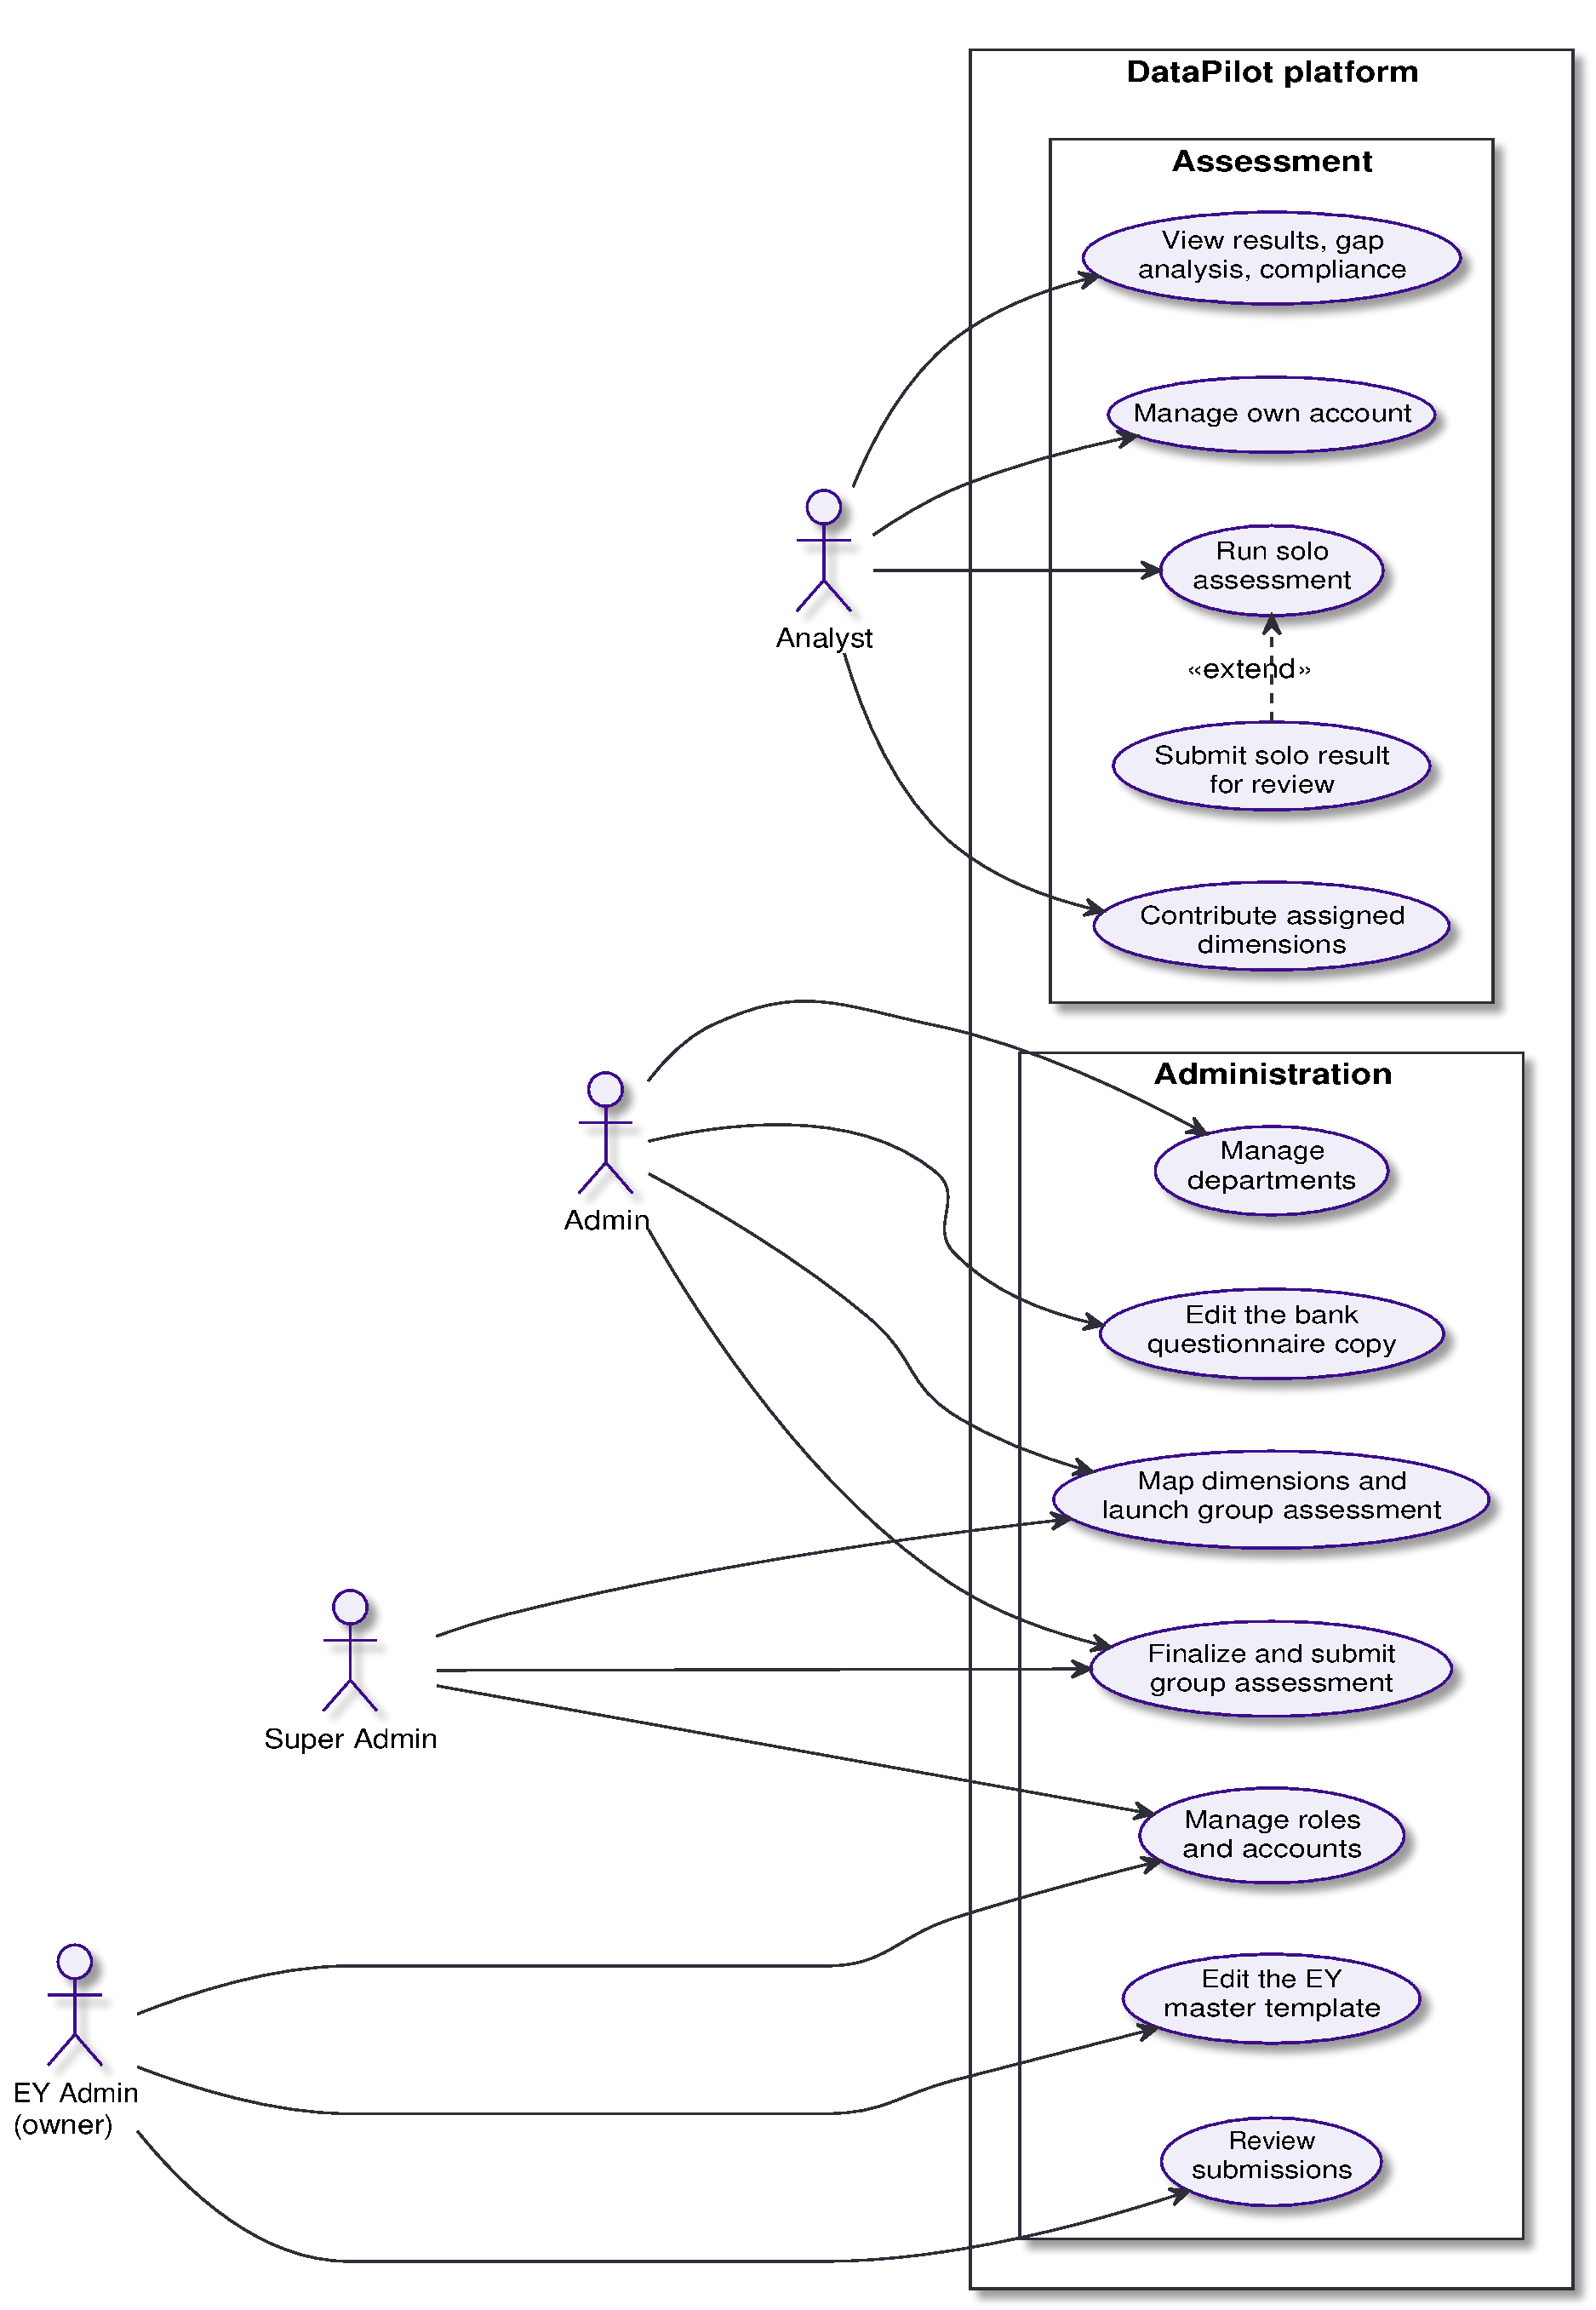
\includegraphics[width=\textwidth]{images/usecase.pdf}
\caption{Use case diagram of DataPilot}
\label{fig:usecase}
\end{figure}

The interactions summarized in the use case diagram of Figure~\ref{fig:usecase} are specified in detail below. Each use case is grounded in the actual behavior of the tool, including the completion gate, the evidence cap, the skip limit, and the non-skippable status of the regulatory indicators. Use cases Use Case 1 to Use Case 11 (Tables~\ref{tab:uc01} to~\ref{tab:uc11}) specify the assessment workflow as it was built in Iteration 3, and they remain valid for the solo assessment path of the platform, with the difference that the profile fields of Use Case 1 are now supplied by the analyst's invited account and shown read-only on the Welcome screen. Two actors participate in them: the Assessor, typically a data or compliance officer who enters the responses, and Management, who consults the resulting dashboards. The Assessor performs the data entry use cases, while both actors consult the results, the roadmap, and the compliance view. The questionnaire itself is not a forced linear wizard: it can be traversed freely through the dimension tabs and the sub-dimension pills, each showing its completion status, and the completion gate is the only ordering constraint in the tool. Three further use cases cover the lifecycle of the session itself: the guarded reset, the undoing of a skip, and the resumption of a persisted session (Use Case 9 to Use Case 11). Use cases Use Case 12 to Use Case 16 (Tables~\ref{tab:uc12} to~\ref{tab:uc16}) then cover the platform interactions introduced by Iteration 4, where the actor set grows from the Assessor and Management to the four platform roles: EY Admin (owner), Super Admin, Admin, and Analyst.

\begin{table}[H]
\centering
\begin{tabular}{|p{3cm}|p{12cm}|}
\hline
\textbf{Actor} & Assessor \\
\hline
\textbf{Preconditions} & The tool is open on the Welcome screen or the Profile screen. \\
\hline
\textbf{Main flow} & 1. The Assessor enters the bank name, the date, the respondent name, and the role. 2. The Assessor confirms the profile. 3. The tool stores the profile and opens the Questionnaire screen. \\
\hline
\textbf{Alternate flows} & 1a. On the Welcome screen the start action stays disabled until all four fields are filled; on the Profile screen the save action stays disabled if the bank name or the respondent name is missing. \\
\hline
\textbf{Postconditions} & The institution profile is recorded and persisted, and the assessment is ready for indicator evaluation. \\
\hline
\end{tabular}
\caption{Use Case 1: Configure assessment}
\label{tab:uc01}
\end{table}

\begin{table}[H]
\centering
\begin{tabular}{|p{3cm}|p{12cm}|}
\hline
\textbf{Actor} & Assessor \\
\hline
\textbf{Preconditions} & The profile is configured and the Questionnaire screen is open. \\
\hline
\textbf{Main flow} & 1. The Assessor selects an indicator. 2. The Assessor reads the question, the hint, and the five level rubric. 3. The Assessor selects a score from one to five. 4. The Assessor enters the supporting evidence in the evidence field. 5. The tool records the score and the evidence and updates the progress indicator. \\
\hline
\textbf{Alternate flows} & 4a. If the score is three or higher and no evidence is entered, the effective score is capped at two by the evidence cap and the indicator is flagged as capped. \\
\hline
\textbf{Postconditions} & The indicator carries a score and an evidence text, and the affected dimension score is recomputed. \\
\hline
\end{tabular}
\caption{Use Case 2: Score an indicator with evidence}
\label{tab:uc02}
\end{table}

\begin{table}[H]
\centering
\begin{tabular}{|p{3cm}|p{12cm}|}
\hline
\textbf{Actor} & Assessor \\
\hline
\textbf{Preconditions} & A non-regulatory indicator is selected on the Questionnaire screen. \\
\hline
\textbf{Main flow} & 1. The Assessor requests to skip the indicator because it does not apply. 2. The tool marks the indicator as skipped and excludes it from the denominators of its sub-dimension and dimension. \\
\hline
\textbf{Alternate flows} & 1a. If the indicator is one of the thirteen regulatory indicators, the skip control is unavailable and the request is refused. 1b. If the dimension has already reached its skip limit, computed as its indicator count multiplied by 20\% and rounded down, the request is refused. \\
\hline
\textbf{Postconditions} & The indicator is either excluded from scoring or left unchanged when a rule refuses the skip. \\
\hline
\end{tabular}
\caption{Use Case 3: Skip a non-regulatory indicator}
\label{tab:uc03}
\end{table}

\begin{table}[H]
\centering
\begin{tabular}{|p{3cm}|p{12cm}|}
\hline
\textbf{Actor} & Assessor, Management \\
\hline
\textbf{Preconditions} & Every dimension of the questionnaire is complete. \\
\hline
\textbf{Main flow} & 1. The actor opens the Results screen. 2. The tool computes the Global Maturity Index, its percentage, and the maturity level. 3. The tool displays the radar chart, the dimension bars, the computation formula, and the interpretation grid. \\
\hline
\textbf{Alternate flows} & 1a. If the assessment is not complete, the completion gate redirects the actor back to the Questionnaire screen. \\
\hline
\textbf{Postconditions} & The maturity profile is displayed for interpretation. \\
\hline
\end{tabular}
\caption{Use Case 4: View maturity results}
\label{tab:uc04}
\end{table}

\begin{table}[H]
\centering
\begin{tabular}{|p{3cm}|p{12cm}|}
\hline
\textbf{Actor} & Assessor, Management \\
\hline
\textbf{Preconditions} & The assessment is complete. \\
\hline
\textbf{Main flow} & 1. The actor opens the Gap Analysis screen. 2. The tool ranks the sub-dimensions by ascending score and assigns each sub-dimension one of four priority labels, from critical to low. 3. The tool groups the labelled sub-dimensions into the three time-sequenced roadmap phases, selecting the recommended actions of each dimension from the band that matches its score, and forces any sub-dimension carrying a failing regulatory indicator or scoring below 2.0 into the first phase. \\
\hline
\textbf{Alternate flows} & 1a. If the assessment is not complete, the completion gate redirects the actor to the Questionnaire screen. \\
\hline
\textbf{Postconditions} & A prioritized, phased set of improvement actions is displayed. \\
\hline
\end{tabular}
\caption{Use Case 5: Review improvement roadmap}
\label{tab:uc05}
\end{table}

\begin{table}[H]
\centering
\begin{tabular}{|p{3cm}|p{12cm}|}
\hline
\textbf{Actor} & Assessor, Management \\
\hline
\textbf{Preconditions} & The assessment is complete. \\
\hline
\textbf{Main flow} & 1. The actor opens the Compliance screen. 2. The tool evaluates the effective score of each of the thirteen regulatory indicators. 3. The tool classifies each as compliant, non compliant, or pending, and computes the compliance rate and the exposure level. 4. The tool displays the statuses, the supporting evidence, the rate, and the exposure. \\
\hline
\textbf{Alternate flows} & 1a. If the assessment is not complete, the completion gate redirects the actor to the Questionnaire screen. \\
\hline
\textbf{Postconditions} & The regulatory posture against the BCT and BCBS 239 requirements is displayed. \\
\hline
\end{tabular}
\caption{Use Case 6: View BCT compliance}
\label{tab:uc06}
\end{table}

\begin{table}[H]
\centering
\begin{tabular}{|p{3cm}|p{12cm}|}
\hline
\textbf{Actor} & Assessor \\
\hline
\textbf{Preconditions} & The Results screen or the Compliance screen is open on a complete assessment. \\
\hline
\textbf{Main flow} & 1. The Assessor requests an export. 2. The tool renders the current dashboard, on the Results screen the maturity report and on the Compliance screen the regulatory report and evidence package, into a printable document. 3. The Assessor saves or prints the document. \\
\hline
\textbf{Alternate flows} & None. \\
\hline
\textbf{Postconditions} & An exportable document capturing the assessment or the compliance evidence is produced. \\
\hline
\end{tabular}
\caption{Use Case 7: Export evidence package}
\label{tab:uc07}
\end{table}

\begin{table}[H]
\centering
\begin{tabular}{|p{3cm}|p{12cm}|}
\hline
\textbf{Actor} & Assessor, Management \\
\hline
\textbf{Preconditions} & The Results screen is open on a complete assessment. \\
\hline
\textbf{Main flow} & 1. The actor selects a target maturity level from one to five. 2. The tool stores the target and overlays it on the radar chart and the dimension bars, exposing the gap between the current and the target profile. \\
\hline
\textbf{Alternate flows} & None. \\
\hline
\textbf{Postconditions} & The target level is persisted and the gap to target is visualized. \\
\hline
\end{tabular}
\caption{Use Case 8: Set target maturity level}
\label{tab:uc08}
\end{table}

\begin{table}[H]
\centering
\begin{tabular}{|p{3cm}|p{12cm}|}
\hline
\textbf{Actor} & Assessor \\
\hline
\textbf{Preconditions} & The Profile screen is open and an assessment, complete or in progress, is stored. \\
\hline
\textbf{Main flow} & 1. The Assessor requests a full reset. 2. The tool opens a confirmation dialog warning that the bank profile and all questionnaire answers, including saved progress, will be permanently deleted and that the action cannot be undone. 3. The Assessor confirms. 4. The tool clears the profile, the answers, and the target level, restores the default state, and empties the persisted assessment in the browser local storage. \\
\hline
\textbf{Alternate flows} & 3a. If the Assessor cancels, or closes the dialog, the assessment is left unchanged. \\
\hline
\textbf{Postconditions} & The tool is returned to its initial unconfigured state and a new assessment can begin. \\
\hline
\end{tabular}
\caption{Use Case 9: Reset the assessment}
\label{tab:uc09}
\end{table}

\begin{table}[H]
\centering
\begin{tabular}{|p{3cm}|p{12cm}|}
\hline
\textbf{Actor} & Assessor \\
\hline
\textbf{Preconditions} & A non-regulatory indicator is currently marked as skipped on the Questionnaire screen. \\
\hline
\textbf{Main flow} & 1. The Assessor selects the undo skip control on the skipped indicator. 2. The tool clears the skipped flag, so the indicator becomes answerable again and its score picker, evidence field, and rubric are restored. 3. The skip counter of the dimension decreases, freeing one skip within the dimension ceiling. \\
\hline
\textbf{Alternate flows} & None. \\
\hline
\textbf{Postconditions} & The indicator is pending again; once scored it re-enters the denominators of its sub-dimension and dimension. \\
\hline
\end{tabular}
\caption{Use Case 10: Undo a skip}
\label{tab:uc10}
\end{table}

\begin{table}[H]
\centering
\begin{tabular}{|p{3cm}|p{12cm}|}
\hline
\textbf{Actor} & Assessor \\
\hline
\textbf{Preconditions} & A previous session stored a profile and answers in the browser local storage under the key \texttt{datapilot-assessment}. \\
\hline
\textbf{Main flow} & 1. The Assessor reopens the tool in the same browser, after a page reload or after closing the browser entirely. 2. The tool rehydrates the profile, the answers, the target level, and the active dimension and sub-dimension from the local storage. 3. The Assessor continues the questionnaire from where the session left off, with all scores, evidence texts, and skips preserved. \\
\hline
\textbf{Alternate flows} & 2a. If no persisted assessment exists, the tool starts with an empty state and the Assessor begins a new session from the Welcome screen. \\
\hline
\textbf{Postconditions} & The session state is identical to the state at the moment it was suspended, and all derived scores recompute to the same values. \\
\hline
\end{tabular}
\caption{Use Case 11: Resume a persisted session}
\label{tab:uc11}
\end{table}

\begin{table}[H]
\centering
\begin{tabular}{|p{3cm}|p{12cm}|}
\hline
\textbf{Actor} & EY Admin (owner), Super Admin, or Admin \\
\hline
\textbf{Preconditions} & The inviter is signed in with an enabled account of the Admin tier or above. \\
\hline
\textbf{Main flow} & 1. The inviter enters the invitee's email and function; the EY Admin also names the bank, creating or reusing the tenant; an Admin inviting an Analyst may optionally attach a department belonging to the bank. 2. The platform fixes the invited role to exactly one rank below the inviter, sends the invitation email, and creates the profile with the inherited bank and the invitation lineage. 3. The invitee follows the link and sets a password. \\
\hline
\textbf{Alternate flows} & 2a. A requested role other than one rank down is refused. 2b. A department belonging to another bank is refused. 2c. An Analyst cannot invite at all. \\
\hline
\textbf{Postconditions} & The new account exists in the inviter's bank (or the named bank), with no identity typed by the invitee. \\
\hline
\end{tabular}
\caption{Use Case 12: Invite a user (per-role)}
\label{tab:uc12}
\end{table}

\begin{table}[H]
\centering
\begin{tabular}{|p{3cm}|p{12cm}|}
\hline
\textbf{Actor} & Admin (bank copy) or EY Admin (owner) (master template) \\
\hline
\textbf{Preconditions} & The bank copy has been created from the EY master template, or the EY Admin edits the master itself. \\
\hline
\textbf{Main flow} & 1. The editor edits dimension names, weights, descriptions, and colors. 2. The editor edits indicator questions, hints, five level rubrics, and the regulatory flag. 3. The editor adds or removes dimensions, sub-dimensions, and indicators. 4. The changes apply to that bank's copy only; edits to the master seed future bank copies. \\
\hline
\textbf{Alternate flows} & 1a. A Super Admin sees the content read-only. 1b. The scoring rules (evidence cap, skip ceiling, compliance thresholds, maturity bands, five level scale) are not editable anywhere. \\
\hline
\textbf{Postconditions} & The bank's bank copy is what its analysts see, and all scores are computed live against it. \\
\hline
\end{tabular}
\caption{Use Case 13: Edit the bank questionnaire}
\label{tab:uc13}
\end{table}

\begin{table}[H]
\centering
\begin{tabular}{|p{3cm}|p{12cm}|}
\hline
\textbf{Actor} & Admin or Super Admin (coordinator) \\
\hline
\textbf{Preconditions} & The bank has departments defined and a questionnaire copy in place. \\
\hline
\textbf{Main flow} & 1. The coordinator creates the shared draft with an optional title; at most one open draft exists per bank, and an existing draft is reused. 2. The coordinator maps each dimension of the bank's questionnaire to exactly one department, optionally applying the suggested Tunisian mapping. 3. The analysts of the mapped departments gain access to their dimensions. \\
\hline
\textbf{Alternate flows} & 2a. Dimensions left unmapped are not writable by anyone and, if never answered, drop out of the index through weight renormalization. \\
\hline
\textbf{Postconditions} & The draft is live and department contributions can begin. \\
\hline
\end{tabular}
\caption{Use Case 14: Map dimensions to departments and launch a group assessment}
\label{tab:uc14}
\end{table}

\begin{table}[H]
\centering
\begin{tabular}{|p{3cm}|p{12cm}|}
\hline
\textbf{Actor} & Analyst (with a department) \\
\hline
\textbf{Preconditions} & The bank has an open group assessment draft with at least one dimension mapped to the analyst's department. \\
\hline
\textbf{Main flow} & 1. The analyst opens the group assessment view and sees only the assigned dimensions. 2. The analyst scores each indicator with evidence under exactly the same rules as the solo path: the evidence cap, the per-dimension skip ceiling, and the non-skippable regulatory indicators. 3. Every change is saved to the shared draft automatically. \\
\hline
\textbf{Alternate flows} & 2a. A write to an indicator outside the assigned dimensions is rejected by the data layer. 2b. Once the assessment is finalized, the view is read-only. \\
\hline
\textbf{Postconditions} & The department's part of the shared answer map is complete, and the coordinator can finalize. \\
\hline
\end{tabular}
\caption{Use Case 15: Contribute assigned dimensions}
\label{tab:uc15}
\end{table}

\begin{table}[H]
\centering
\begin{tabular}{|p{3cm}|p{12cm}|}
\hline
\textbf{Actor} & Admin or Super Admin (coordinator) \\
\hline
\textbf{Preconditions} & An open group assessment draft exists with at least one scored indicator. \\
\hline
\textbf{Main flow} & 1. The coordinator confirms the finalization. 2. The platform re-reads all answers from the server and computes the scores with the same engine as the solo path. 3. The platform records an immutable submission for the bank, marked as a multi-department group assessment. 4. The platform atomically flips the draft to finalized. \\
\hline
\textbf{Alternate flows} & 2a. Finalization is refused when nothing has been scored. 4a. If another coordinator finalized concurrently, the attempt reports that the assessment was already finalized and leaves exactly one submission. \\
\hline
\textbf{Postconditions} & The answers are locked read-only at the data layer, and the submission appears in the bank's submissions review and to EY. \\
\hline
\end{tabular}
\caption{Use Case 16: Finalize and submit a group assessment}
\label{tab:uc16}
\end{table}

\subsection{Conclusion}

This chapter presented the four iterations through which the framework, the scoring methodology, the DataPilot tool, and the multi-tenant platform were designed, validated, implemented, and evaluated, each following the DSR regulative cycle. The next chapter presents the consolidated results and findings and answers the research questions.
